\chapter{\label{ch:3}Maschinelle Übersetzung}

\section{\label{sec:3.0}Einleitung}

Mit der stetigen Zunahme der zu übersetzenden Datenmenge stieg auch der Bedarf an maschinellen Übersetzungen (MÜ). Viele Unternehmen integrieren heutzutage die MÜ in ihren Übersetzungsprozess und versuchen mit der Einbettung eines anschließenden Post-Editing-Schritts in ihren Workflow, die Übersetzungsproduktivität zu erhöhen und gleichzeitig die Übersetzungskosten zu reduzieren. Dieser Bedarf gekoppelt mit steigenden Qualitätsansprüchen führt dazu, dass MÜ-Systeme ständig unter die Lupe genommen werden. Das vorliegende Kapitel beschäftigt sich mit der Entwicklung, den Ansätzen und der Qualitätsbewertung der MÜ. Auf die Definition der MÜ und eine Erläuterung ihrer Relation zu der Kontrollierten Sprache (KS) folgt eine Darstellung der verschiedenen MÜ-Ansätze. Anschließend befasst sich das Kapitel mit der Thematik der MÜ-Qualität und den verschiedenen Qualitätsbewertungstechniken. Zum Schluss werden MÜ-Studien im Kontext der KS diskutiert; auch die geringe Anzahl der KS-Untersuchungen auf Regelebene und die Herausforderungen solcher Untersuchungen werden näher betrachtet.

\section{\label{sec:3.1}MÜ – Begriffsbestimmung und Motiv des KS-Einsatzes}

Die maschinelle Übersetzung wird als „der Prozess der automatischen Übersetzung von Text aus einer natürlichen Sprache in eine andere“ definiert \citep{DorrEtAl1999}. Inwiefern MÜ-Systeme selbständig bzw. ohne menschliche Intervention funktionieren können, ist ein wesentlicher Punkt von vielen Definitionen der MÜ. Im Jahr 1987 definierte Goshawke die MÜ als

\begin{quote}
the transfer of meaning from one natural (human) language to another with the aid of a computer. There are very few systems that are, or even attempt to be, complete machine translation systems in themselves -- nearly all systems are Machine Aided Translation (MAT), involving human help either at the input stage (pre-editing) or the output stage (post-editing) or both. \citep[6]{Goshawke1987}
\end{quote}

Auch bei \citep[3]{HutchinsSomers1992} ist das menschliche Eingreifen ein Bestandteil der Definition der MÜ-Systeme, so seien „computerized systems responsible for the production of translations from one natural language into another, with or without human assistance“. Ein Verzicht auf die menschliche Intervention in der MÜ ist bisher als unrealistisch zu betrachten. In den 50er Jahren kritisierte Yehoshua Bar-Hillel die Annahme, dass eine Fully Automatic High Quality Translation (FAHQT) das Ziel der MÜ sei (ebd.:~6f.). Nach wie vor bezeichnet man den MÜ-Output als Rohübersetzung und versucht mithilfe des Pre-Editing bzw. des Post-Editing diesen Rohoutput zu verbessern und die Übersetzungsproduktivität zu erhöhen.

Gleichzeitig erlebte die MÜ-Entwicklung große technologische Sprünge von einem Ansatz zum anderen – angefangen bei den regelbasierten Systemen über die statistischen und hybriden Systeme bis hin zu den neuronalen Systemen. Mit dieser Entwicklung verbesserte sich der MÜ-Output in den verschiedenen Domänen zu einem unterschiedlichen Grad. Der Qualitätsunterschied des MÜ-Outputs ist leicht erkennbar, wenn man in einem Extremfall einen Abschnitt aus einem Benutzerhandbuch und ein kurzes Gedicht maschinell übersetzt. Die MÜ-Qualität des technischen Texts fällt in der Regel viel höher als die des Literarischen aus. Wenn ein MÜ-System theoretisch in der Lage ist, eine hohe Qualität zu liefern, warum ist dies nicht immer realisierbar? \citet[2]{HutchinsSomers1992} geben eine schlüssige Antwort auf diese Frage: „The major obstacles to translating by computer are, as they have always been, not computational but linguistic.“ Je einfacher der Text auf linguistischer Ebene ist, desto höher fällt die Qualität seiner MÜ aus. Dementsprechend wurde durch die Anwendung von Pre-Editing-Techniken wie der Kontrollierten Sprache daran gearbeitet, durch die Vermeidung von Ambiguität, Vereinfachung der Satzstruktur und Einschränkung bzw. Standardisierung der Lexik, die Komplexität des Ausgangstexts zu reduzieren. Bereits in der ersten Konferenz für MÜ 1952 umfassten die Pläne und Anregungen für zukünftige Forschung das Schreiben in Kontrollierten Sprachen, die Konstruktion von Subsystemen sowie die Anerkennung des Bedarfs an menschlicher Unterstützung in Form von Pre- und Post-Editing (ebd.: 6).

In der vorliegenden Arbeit liegt der Fokus auf dem Einsatz der Kontrollierten Sprache (KS) und ihrem Einfluss auf den MÜ-Output. Durch einen Vergleich der unterschiedlichen MÜ-Ansätze wird in der Arbeit untersucht, ob und inwiefern die analysierten Regeln der KS heutzutage die MÜ-Qualität verbessern können und somit den menschlichen Eingriff in den Übersetzungsprozess reduzieren.

\section{\label{sec:3.2}Entwicklung der MÜ-Ansätze}

Die Forschung in diesem Bereich begann nach dem Zweiten Weltkrieg, zunächst mit dem Ziel, russische Texte ins Englische zu „decodieren“. Die Begriffe, die damals aus der Kryptographie entlehnt wurden, werden bis heute weiterhin verwendet. Leon Dostert arbeitete 1954 an der Georgetown Universität gemeinsam mit IBM an einem Projekt, im Rahmen dessen sorgfältig ausgewählte russische Beispielsätze mit einem sehr begrenzten Vokabular von 250 Wörtern und sechs Grammatikregeln ins Englische übersetzt wurden (\citealt{HutchinsSomers1992}:~6). Dem lag die Idee zugrunde, auf diese Weise die technische Durchführbarkeit der MÜ nachzuweisen. Die ersten entwickelten Systeme waren regelbasiert, gefolgt von den SMÜ-Systemen. Um von den Vorteilen der beiden Ansätze zu profitieren, wurden hybride Systeme entwickelt, die auf regelbasierten und statistischen Komponenten beruhen. Der aktuellste MÜ-Ansatz ist der neuronale Ansatz, der von dem massiven Volumen der gesammelten Daten profitiert und auf Basis von neuronalen Netzen arbeitet. In dieser Studie wurden MÜ-Systeme verwendet, die nach den folgenden Ansätzen konzipiert sind: ein regelbasiertes MÜ-System (RBMÜ), ein statistisches MÜ-System (SMÜ), zwei hybride MÜ-Systeme (HMÜ) und ein neuronales MÜ-System (NMÜ).\footnote{Die Auswahlkriterien der untersuchten MÜ-Systeme sind unter \sectref{sec:4.4.1} aufgeführt.} Im Folgenden werden die Entwicklung dieser Ansätze -- chronologisch -- dargestellt sowie deren zugrundeliegenden Paradigmen genauer erläutert.

\subsection{Regelbasierte MÜ-Systeme}
\label{sec:3.2.1}
Hauptmerkmal der RBMÜ ist, dass dabei das System auf linguistische Regeln zurückgreift \citep[38]{Ramlow2008}. Das System analysiert den Text auf verschiedenen linguistischen Ebenen, z.~B. die Kasusflexionen auf morphologischer Ebene und Wortstellung auf syntaktischer Ebene. Danach -- je nach RBMÜ-Methode -- überführt das System den Ausgangstext in eine abstrakte Repräsentation. Anschließend wendet das System zur Produktion des Zieltexts Übersetzungsregeln an. (\citealt{WerthmannWitt2014}: 87)

Die ersten MÜ-Systeme waren regelbasiert. In den 60er Jahren entwickelte die Saarbrücken-Gruppe ein mehrsprachiges „Transfersystem“ namens SUSY. 1976 wurde Systran als RBMÜ-System von der EU-Kommission für die Übersetzung im Sprachenpaar Englisch-Französisch installiert und in den darauffolgenden Jahren um andere Sprachenpaare erweitert. In den 80er Jahren wurden ebenfalls die ersten RBMÜ-Systeme für die Sprachenkombination Englisch-Japanisch entwickelt. (\citealt{HutchinsSomers1992}: 7f.)

Die Architektur eines RBMÜ-Systems lässt sich mithilfe des Dreiecks von Vauquois anschaulich darstellen \citep{Vauquois1968}:


\begin{figure}

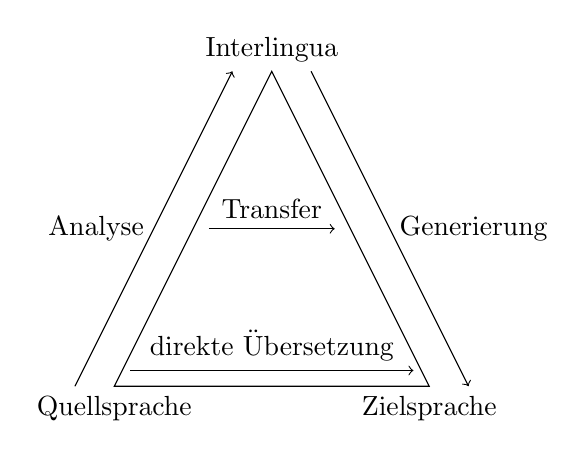
\begin{tikzpicture}
\draw (0,2) node[above]{Interlingua} -- (-2, -2) node[below]{Quellsprache} -- (2, -2) node[below]{Zielsprache} -- cycle;
\draw[->] (-2.5, -2) -- (-0.5, 2) node[pos=.5, left]{Analyse};
\draw[->] (0.5, 2) -- (2.5, -2) node[pos=.5, right]{Generierung};
\draw[->] (-0.8, 0) -- (0.8, 0) node[pos=.5, above]{Transfer};
\draw[->] (-1.8, -1.8) -- (1.8, -1.8) node[pos=.5, above]{direkte Übersetzung};

\end{tikzpicture}
\caption{Vauquois-Dreieck der MÜ-Systemparadigmen. Quelle: \citealt{HutchinsSomers1992}: 107}
\label{fig:3:1}
\end{figure}


In diesem Schema steigt die Systemkomplexität, je mehr man sich im Dreieck nach oben bewegt, von bloßen Wörtern über syntaktische Übertragungsregeln bis hin zu einer vollständig sprachunabhängigen Repräsentation (Interlingua). Wie das Dreieck von Vauquois zeigt, entwickelte sich der RBMÜ-Ansatz im Laufe der Zeit von der direkten Methode zu der transferbasierten Methode und anschließend zur Interlingua-Methode. Die Unterscheidungsmerkmale bei den Methoden sind die Anzahl der Sprachenpaare, die Analysemethode der aus dem Quelltext gewonnenen Informationen sowie die Methode der abstrakten Repräsentation dieser Informationen für die Übersetzung. (\citealt{WerthmannWitt2014}: 87) Im Folgenden eine kurze Erläuterung der drei Methoden:

\textit{Direkte Übersetzung:} Bei dieser Methode werden die Quellsprachwörter wortweise mithilfe eines zweisprachigen Wörterbuchs in die Zielsprachwörter übersetzt. Die Wortstellung des Outputs erfolgt unter Verwendung einfacher syntaktischer Regeln \citep{Stein2009}. Somit basiert diese Methode auf einer morphologischen Analyse der Wörter und einem komplexen zweisprachigen Wörterbuch sowie einigen einfachen Regeln zur Wortstellung (\citealt{CarstensenEtAl2004}: 566). Es erfolgt keine Tiefenanalyse des Ausgangssatzes und es werden keine komplexen Regeln zur Generierung des Zielsatzes angewendet. Entsprechend ist die Qualität der Übersetzung im Allgemeinen nicht als hoch einzustufen und steigt, je ähnlicher die Ausgangs- und Zielsprachen einander syntaktisch und semantisch sind (\citealt{WerthmannWitt2014}: 88).

\textit{Transferbasierte Methode:} In der transferbasierten Methode findet eine komplexe linguistische Analyse statt und beginnt die Generierung während der Übersetzung. Im Rahmen dieser Methode erfolgt die Übersetzung auf Satz- und nicht auf Wortebene (\citealt{WerthmannWitt2014}: 89). Die Methode besteht aus drei Schritten (\citealt{CarstensenEtAl2010}: 646): Analyse, Transfer und Generierung. Im ersten Schritt wird der Quelltext geparst, segmentiert und syntaktisch bzw. semantisch analysiert. Im zweiten Schritt wird ein Transfer von der syntaktischen/semantischen Repräsentation des Ausgangssatzes in die Repräsentation der Zielsprache unter Verwendung von Mapping-Regeln durchgeführt. Zum Schluss wird der Zielsatz auf Basis der transferierten Repräsentation generiert. (\citealt{WerthmannWitt2014}: 89) Durch die syntaktische und semantische Sprachanalyse ist die Qualität der Übersetzung in der Transfermethode höher als die der direkten Methode \citep{Stein2009}.

\textit{Interlingua-Methode:} Im Gegensatz zu der transferbasierten Methode, die aus\-gangs- und zielsprach abhängige Regeln für den lexikalischen, syntaktischen und semantischen Transfer beinhaltet, arbeitet die Interlingua-Methode mit einer generischen Repräsentation, der sogenannten Interlingua (\citealt{WerthmannWitt2014}: 90). Die Grundidee der Interlingua besteht darin, den Ausgangssatz in einer sprachunabhängigen, abstrakten Begriffsrepräsentation darzustellen, die aus jeder Ausgangssprache erzeugt werden kann und zur Generierung der Übersetzung in eine beliebige Zielsprache verwendet wird (ebd.). Wie das Vauquois-Dreieck zeigt, ist diese Methode im Vergleich zu den anderen Übersetzungsmethoden mit deutlich mehr Aufwand verbunden. Zusammenfassend besteht die Interlingua-Methode aus zwei Schritten (\citealt{CarstensenEtAl2010}: 646): Analyse und Generierung. Im Analyseschritt wird der Ausgangstext geparst, segmentiert und analysiert, um die Interlingua der Ausgangssätze zu erzeugen. Im Generierungsschritt wird der Zieltext aus der Interlingua erzeugt. Entsprechend wird der Vorteil dieser Methode als eng an ihren Nachteil gebunden betrachtet (\citealt{WerthmannWitt2014}: 90f.): Einerseits erspart die ausgangsprachunabhängige Zwischen-repräsentation die Erzeugung von sprachspezifischen lexikalischen, syntaktischen und semantischen Regeln bei jedem Sprachenpaar; andererseits stellt die Realisierung solcher generischen Zwischenrepräsentationen für eine formale Sprache mit eigenen lexikalischen und syntaktischen Elementen eine komplexe Aufgabe dar. Daher wird diese Methode für bestimmte Domänen (z.\,B. Hotelreservierung) oder für kontrollierten Zielsprachen mit eingeschränktem Vokabular und begrenzten Satzstrukturen verwendet \citep{Al-Ansary2011}.


Die Ergebnisqualität der RBMÜ-Systeme variiert von einem Sprachenpaar zum anderen und hängt davon ab, ob eine bestimmte Fachsprache unterstützt wird und die notwendigen Fachtermini eingepflegt sind \citep{Stein2009}. Daher stellt die aufwendige Bereitstellung von zweisprachigen Wörterbüchern und Regelwerken einen Nachteil von RBMÜ-Systemen dar (\citealt{WerthmannWitt2014}: 91). Dies ließ die statistischen MÜ-Systeme seit Ende der 80er Jahre als präzisere und weniger aufwendige Systeme in den Vordergrund rücken (\citealt{TripathiSarkhel2010}).

Im Rahmen dieser Studie wird der KS-Effekt auf den RBMÜ-Output des Systems \textit{Lucy LT} \footnote{\textrm{Link zum System Lucy LT: \url{http://www.lucysoftware.com/english/machine-translation/lucy-lt-kwik-translator-}}} untersucht. Lucy LT (Nachfolger des METAL MÜ-Systems) ist ein transferbasiertes MÜ-System, das mit einem Island-Chart-Parser und in drei Übersetzungsphasen arbeitet (\citealt{MartinSerra2014}): Analyse, Transfer und Generierung. In jeder dieser Phasen und für jede Sprachrichtung werden eine Analysegrammatik, eine Transfergrammatik und eine Generierungsgrammatik sowie Ausgangs- und Zielsprachenlexika und ein Ausgang-zu-Ziel-Transferlexikon verwendet (ebd.).

\subsection{Statistische MÜ-Systeme}
\label{sec:3.2.2}
Anstelle der Bereitstellung von aufwendigen Regelsammlungen zur Erstellung von RBMÜ-Systemen überraschte der IBM-Wissenschaftler Peter Brown 1988 das Publikum auf der zweiten TMI-Konferenz mit dem Konzept der Statistischen MÜ (SMÜ), das auf parallelen Korpora basiert \citep{Stein2009}. Ein reines SMÜ-System verwendet keine linguistischen Informationen \citep{Forcada2010}. Die Grundidee eines SMÜ-Systems besteht darin, dass „a source language and a target language sentence are a translation of each other with a certain probability“ (ebd.: 220). Somit ist das Ziel eines SMÜ-Systems, den entsprechenden Satz in der Zielsprache zu finden, der die höchste Wahrscheinlichkeit aufweist (ebd.).

In der Klassifizierung der MÜ-Ansätze fällt die SMÜ zusammen mit der beispielbasierten MÜ in die Kategorie der korpusbasierten Methoden. Hauptmerkmal dieser Methoden ist die Übersetzung mithilfe eines zweisprachigen Korpus. Der zu übersetzende Satz wird mit dem Korpus abgeglichen, um eine Übersetzungslösung zu finden. In der \textit{beispielbasierten MÜ} greift das System auf Beispielübersetzungen in einem zweisprachigen Korpus zurück und ordnet dem Ausgangssegment das am ehesten vergleichbare Zielsegment zu. Bei der \textit{SMÜ} wird das zweisprachige Korpus, das als Übersetzungsmodell agiert, durch einsprachige Korpora für die beteiligten Sprachen, die als Sprachmodelle fungieren, ergänzt. (\citealt{Ramlow2008}: 42f.)


\newsavebox{\transmodbox}
\savebox{\transmodbox}{
\begin{tikzpicture}[
node distance = 10pt,
corpusnode/.style={draw, cylinder, shape border rotate=90, shape aspect=.15, minimum width=4cm, minimum height=1cm}]
\node(transmod){Translational model};
\node[corpusnode](paracorpus)[below=of transmod]{Parallel corpus};
\end{tikzpicture}
}
% {width("Monolingual corpus")+4pt}
% {height("Monolingual corpus")+4pt}
\newsavebox{\langmodbox}
\savebox{\langmodbox}{
\begin{tikzpicture}[
node distance = 3pt]
\node(langmod){Language model};
\node[cylinder, shape border rotate=90, shape aspect=.15, draw, minimum width=4cm, minimum height=1cm](monocorpus)[below=of langmod]{Monolingual corpus};
\end{tikzpicture}
}

\begin{figure}
\scalebox{.8}{
\begin{tikzpicture}

\node[rectangle, rounded corners, draw, align=center] (decoder) {Decoder\\argmax(P(t)*P(s/t))};
\node[rectangle, draw](pre-pros)[left=of decoder]{Pre-processing};
\node[align=center](source)[left=of pre-pros]{Source\\text};
\node[rectangle, draw](post-pros)[right=of decoder]{Post-processing};
\node[align=center](target)[right=of post-pros]{Target\\text};

\node[draw](transmodbox)[above= of pre-pros]{\usebox\transmodbox};
\node[draw](langmodbox)[above= of post-pros]{\usebox\langmodbox};

%arrows
\draw[->](transmodbox.east)-|(decoder.150) node[pos=.3, above]{P(s/t)};
\draw[->](langmodbox.west)-|(decoder.30) node[pos=.2, above]{P(t)};
\draw[->](source.east)--(pre-pros.west);
\draw[->](pre-pros.east)--(decoder.west);
\draw[->](decoder.east)--(post-pros.west);
\draw[->](post-pros.east)--(target.west);


\end{tikzpicture}
}
\caption{SMÜ-Architektur. Quelle: \citealt{Dubey2017}}
\label{fig:3:2}
\end{figure}


\figref{fig:3:2} veranschaulicht die Architektur eines typischen SMÜ-Systems, das aus den folgenden Komponenten besteht (\citealt{Petrzelka2011}: 8ff.; \citealt{Dubey2017}):

\begin{enumerate}[label = {(\arabic*)}, align = left]%1

\item
         einem \textit{Zielsprachenmodell}, das auf einem einsprachigen Korpus in der Zielsprache basiert und für die korrekte Zusammenstellung der Wörter in der Zielsprache zuständig ist. Es berechnet die Wahrscheinlichkeit des Zielsatzes;


\item

         einem \textit{Übersetzungsmodell}, das auf einem Parallelkorpus basiert und die bedingte Wahrscheinlichkeit des Zielsatzes in Anbetracht des Ausgangssatzes berechnet. Um dies zu realisieren, erfolgt zunächst ein Word-Alignment, bei dem ermittelt wird, welches Wort im Ausgangssatz welchem Wort im Zielsatz entspricht. Auf Basis des Word-Alignments wird ein Phrasen-A\-lign\-ment durchgeführt und die sogenannte ,,Phrasenübersetzungstabelle'' (phrase-translation table) erstellt, d.~h. eine Tabelle, die die Phrasen des Ausgangstexts, die Phrasen des Zieltexts sowie deren Übereinstimmungswahrscheinlichkeit (matching probability) beinhaltet;

\item
         einem \textit{Decoder}, der die eigentliche Übersetzungsaufgabe übernimmt, indem er das bestmögliche Übersetzungspaar durch das Maximieren der zwei zuvor genannten Wahrscheinlichkeiten findet. Je häufiger ein Übersetzungspaar in den Korpora auftritt, desto höher ist sein Ranking.
\end{enumerate}

Man unterscheidet im SMÜ-Ansatz zwischen der wortbasierten und phrasenbasierten SMÜ, je nachdem auf welcher Ebene das Übersetzungsmodell erstellt wird und ob die Wahrscheinlichkeiten für Wörter oder Phrasen berechnet werden (\citealt{WerthmannWitt2014}: 93):

\textit{Wortbasierte SMÜ:} Hierbei erfolgt die Analyse der Korpora auf Wortebene. Der Satz wird in Wörter aufgeteilt und auf Wortebene übersetzt \citep[81]{Köhn2010}. Dementsprechend setzt dieser Ansatz eine 1:1-Beziehung zwischen den Wörtern in der Ausgangs- und Zielsprache voraus, was in der Realität jedoch nicht gegeben ist (\citealt{WerthmannWitt2014}: 94). Daraus entstand die Notwendigkeit der Übersetzung auf Phrasenebene.

\textit{Phrasenbasierte SMÜ (PBMÜ):} Bei diesem Ansatz stellt eine Phrase eine Übersetzungseinheit dar, wobei es sich hier nicht um eine Phrase im linguistischen Sinn handelt, sondern um eine syntaktische Phrase, die aus einer Sequenz von Wörtern besteht (\citealt{Köhn2010}:~128). Sobald die Phrasen in die Zielsprache übersetzt wurden, übernimmt das Sprachmodell seine Aufgabe, nämlich die Phrasen in der richtigen zielsprachigen Reihenfolge zu ordnen (\citealt{CarstensenEtAl2010}: 650). Ein wichtiger Vorteil der phrasenbasierten gegenüber der wortbasierten SMÜ beruht auf der Möglichkeit, ein Wort des Ausgangssatzes mit mehreren Wörtern in den Zielsatz zu übersetzen und umgekehrt (\citealt{WerthmannWitt2014}: 95). Ein sehr bekanntes phrasenbasiertes SMÜ-System ist Moses. In Moses wurde die phrasenbasierte Übersetzung (PBMÜ) um Faktoren und Confusion-Network-Decoding erweitert (\citealt{KöhnEtAl2007}): Ein Factored-Übersetzungsmodell erlaubt die Verwendung morphologischer, syntaktischer und semantischer Informationen. Die Integration des Confusion-Network-Decoding ermöglicht die Übersetzung von mehrdeutigen Inputs, da -- anstatt der bloßen Ermittlung des besten Outputs -- ein Netzwerk von unterschiedlichen Wortoptionen untersucht wird.


Im Vergleich zu den RBMÜ-Systemen sind die SMÜ-Systeme günstiger (\citealt{WerthmannWitt2014}: 95), da die zeitaufwendige Erstellung von Regelwerken entfällt. Wenn Parallelkorpora für weitere Sprachen verfügbar sind, lassen sich die SMÜ-Systeme ohne großen Aufwand um weitere Sprachen erweitern \citep{Stein2009}, jedoch ist die Erstellung von großen alignierten Korpora mit Aufwand verbunden, was als Schwäche der SMÜ betrachtet wird (\citealt{WerthmannWitt2014}: 96).

Im Rahmen dieser Studie wird das SMÜ-System \textit{SDL Free Translation}\footnote{{{{Link zum System SDL Free Translation: \url{https://www.freetranslation.com/de}}}}} untersucht. SDL Free Translation ist ein rein statistisches MÜ-System der Firma SDL.\footnote{Quelle: „What Is Machine Translation and How Does It Work?“, Online unter: \url{https://sdl.uservoice.com/knowledgebase/articles/256030-what-is-machine-translation-and-how-does-it-work} [abgerufen am 06.12.2016].}

\subsection{Hybride MÜ-Systeme}
\label{sec:3.2.3}
Nachdem die RBMÜ als der traditionelle Ansatz der MÜ im Laufe der 90er Jahre durch den SMÜ-Ansatz zunehmend ersetzt wurde, kam die Idee auf, beide Ansätze zu kombinieren, um gleichzeitig von ihren Vorteilen zu profitieren und ihre Schwächen gegenseitig kompensieren zu können. In der hybriden Methode liegt der Fokus auf der Kombinierung der besten Eigenschaften von zwei oder mehr MÜ-Ansätzen, häufig werden dabei Regeln in einen SMÜ-Ansatz integriert (\citealt{Costa-JussàFonollosa2015}).

Entsprechend kam zur Jahrtausendwende der Trend auf, HMÜ-Systeme zu entwickeln. \citet{Cavalli-SforzaLavie2006} beschreiben die Verbreitung von hybriden Systemen sowohl in der Forschung als in der Industrie wie folgt:

\begin{quote}
Much current research in machine translation is neither based purely on linguistic knowledge nor on statistics, but includes some degree of hybridization. At AMTA 2004 and MT Summit 2005 just about all commercial MT developers also claimed to have hybrid systems. (\citealt{Cavalli-SforzaLavie2006}: 1)
\end{quote}

Die hybriden Systeme werden unterschiedlich aufgebaut; sie beinhalten verschiedene RBMÜ- und SMÜ-Komponenten. Das System kann z. B. Module enthalten, in denen die Wörterbücher und Regeln des Systems sich je nach Übersetzungsdomäne (IT, Technik, Medizin) dynamisch anpassen. Eine weitere Aufbaumöglichkeit ist der Einsatz eines statistischen Ansatzes zur Unterstützung bei einer korrekten Übersetzung auf Wortebene (z.~B. das Wort „Maus“ in der IT- vs. Zoologie-Domäne). \citep[171]{Poibeau2017}

Aufgrund der Diversität der Aufbaumöglichkeiten existieren mehrere Klassifizierungen für die HMÜ-Systeme. \citet{Eisele2007} unterscheidet bei der Hybridisation zwischen einer flachen Integration, in der zwei oder mehr Systeme in einem größeren System integriert werden, und einer tiefen Integration, in der die Vorteile von zwei Ansätzen zusammengeführt werden. Eine andere Klassifizierung von \citet{Way2010} unterscheidet zwischen einem Multi-Engine-Ansatz und einem integrierten Systemansatz. Dennoch, wie oben erwähnt, sind die meisten hybriden Systeme eine Kombination von RBMÜ- und SMÜ-Systemen. Daher wäre es an dieser Stelle sinnvoll zwischen zwei Varianten der Hybridisation zu unterscheiden (\citealt{Costa-JussàFonollosa2015}): (1) ein RBMÜ-System, das mit Data ergänzt wurde (eine RBMÜ-geführte Hybridisation) und (2) ein SMÜ-System, das mit linguistischen Regeln ergänzt wurde (eine SMÜ-geführte Hybridisation).

\textit{RBMÜ-geführte Hybridisation:} Diese Art von Hybridisation kann auf mehrere Weise realisiert werden, z.~B. durch die Einführung eines Korpus zum Aufbau des RBMÜ-Systems, die Einführung von korpusbasierten Tools zur Gewichtung des RBMÜ-Outputs oder die Durchführung eines statistischen Post-Editing für den RBMÜ-Output (ebd.).


\begin{figure}
\scalebox{.7}{
\begin{tikzpicture}[
node distance = 15pt,
align=center,
whitenode/.style={draw, rectangle, draw=black, thin, minimum height=30pt, minimum width=1.7cm},
graynode/.style={draw, rectangle, draw=black, fill=gray!10, thin, minimum height=30pt, minimum width=2cm},
blanknode/.style={minimum height=30pt, minimum width=2cm}
]

\node[graynode] (trans) {Transference};
%left nodes
\node[whitenode](smt)[left=of trans]{SMT\\Enrichment};
\node[graynode] (an)[left=of smt] {Analysis};
\node[blanknode](source)[left=of an]{Source\\sentence};
%above
\node(corpl)[above=of smt]{CORPORA};
%right nodes
\node[graynode](gen)[right=of trans]{Generation};
\node[whitenode](decode)[right=of gen]{Decoding};
\node[blanknode](target)[right=of decode]{Target\\sentence};
%above
\node(corpr)[above=of decode]{CORPORA};

%arrows
\draw[->](source.east)--(an.west);
\draw[->](an.east)--(smt.west);
\draw[->](smt.east)--(trans.west);
\draw[->](trans.east)--(gen.west);
\draw[->](gen.east)--(decode.west);
\draw[->](decode.east)--(target.west);
\draw[->](corpl.south)--(smt.north);
\draw[->](corpr.south)--(decode.north);


\end{tikzpicture}
}
\caption{RBMÜ-geführte Hybridisation. Quelle: \citealt{Costa-JussàFonollosa2015}}
\label{fig:3:3}
\end{figure}


Die RBMÜ wurde kritisiert, dass der RBMÜ-Output im Vergleich zum SMÜ-Output oft weniger natürlich und flüssig klingt, da RBMÜ-Systeme keinen Zugriff auf statistische Sprachmodelle haben. Diese Schwäche wird im hybriden Ansatz durch die Integration eines Flüssigkeitsmodells in die RBMÜ-Architektur mittels Post-Editing behandelt. Auf diese Weise konnte der MÜ-Output eines reinen RBMÜ-Systems im Hinblick auf die Flüssigkeit und die Kontextualität verbessert werden. \citep{EiseleEtAl2008}

\textit{SMÜ-geführte Hybridisation:} Diese Art von Hybridisation erfolgt durch die Kombinierung verschiedener korpusbasierter MÜ-Ansätze oder durch die Integration von Regeln in ein korpusbasiertes MÜ-System, und zwar mittels der Verwendung von Regeln bei dem Pre-/Post-Editing oder der Integration von Wörterbüchern bzw. Regeln in das Kernmodell (\citealt{Costa-JussàFonollosa2015}).


\begin{figure}
\scalebox{.8}{
\begin{tikzpicture}[
node distance = 15pt,
align=center,
whitenode/.style={draw, rectangle, draw=black, thin, minimum height=30pt, minimum width=1.7cm},
graynode/.style={draw, rectangle, draw=black, fill=gray!10, thin, minimum height=30pt, minimum width=2cm},
blanknode/.style={minimum height=30pt, minimum width=2cm}
]

\node[graynode] (decode) {Decoding};
%left nodes
\node[whitenode](rec)[left=of decode]{Recording\\Rules};
\node[graynode] (pre)[left=of rec] {Pre-\\processing};
\node[blanknode](source)[left=of pre]{Source\\sentence};
%above
\node(stat)[above=of decode]{STATISTICAL MODELS};
%right nodes
\node[graynode](post)[right=of decode]{Post-\\processing};
\node[blanknode](target)[right=of post]{Target\\sentence};

%arrows
\draw[->](source.east)--(pre.west);
\draw[->](pre.east)--(rec.west);
\draw[->](rec.east)--(decode.west);
\draw[->](decode.east)--(post.west);
\draw[->](post.east)--(target.west);
\draw[->](stat.south)--(decode.north);


\end{tikzpicture}
}
\caption{SMÜ-geführte Hybridisation. Quelle: \citealt{Costa-JussàFonollosa2015}}
\label{fig:3:4}
\end{figure}


Die Ergänzung von SMÜ-Systemen um syntaktische Analysen oder semantische Operationen kann insbesondere bei Sprachenpaaren, für die keine großen Korpora verfügbar sind oder deren Satzbau und Flexion sich stark unterscheiden, von Vorteil sein \citep{Stein2009}.

Zusammenfassend wird in den verschiedenen Hybridarchitekturen in der Regel entweder eine RBMÜ-Engine verwendet, um die für den SMÜ-Decoder verfügbaren lexikalischen Ressourcen anzureichern; oder es werden Komponenten der SMÜ-Infrastruktur zusammen mit linguistischer Verarbeitung und manueller Validierung verwendet, um das Lexikon einer RBMÜ-Engine zu erweitern (vgl. \citealt{EiseleEtAl2008}). Je nach Art der Kombination der Hybridstruktur, kann ein HMÜ-System in verschiedenen Szenarien unterschiedliche Stärken und Schwächen zeigen.

Aufgrund der Aufbaudiversität in diesem MÜ-Ansatz wurden in dieser Studie zwei verschiedene Hybridsysteme untersucht: \textit{Systran} und \textit{Bing Translator}.\footnote{Links zu den Systemen Systran und Bing Translator:
\url{http://www.systranet.com/translate},
\url{https://www.bing.com/translator}
}
Bing Translator ist ein „statistisches MÜ-System mit sprachspezifischen Regelkomponenten für das Zerlegen und Zusammensetzen von Sätzen“ (\citealt{WerthmannWitt2014}: 84), das von Microsoft Übersetzer angetrieben wird. Systran wurde ursprünglich als RBMÜ entwickelt und erst 2009 durch die Ergänzung um statistische Komponenten zu einem Hybridsystem weiterentwickelt (ebd.: 99).

\subsection{Neuronale MÜ-Systeme}
\label{sec:3.2.4}
Nach dem Fortschritt, den die SMÜ bis zum Ende des 20. Jahrhunderts verzeichnete, waren keine weiteren Durchbrüche zu beobachten. Die SMÜ erreichte eine Stufe, nach der eine markante Verbesserung schwer realisierbar war. So gaben die Forscher von Google Translate im Jahr 2010 im „Guardian“ zu, dass

\begin{quote}
the idea that more and more data can be introduced to make the system better and better is probably a false premise. Each doubling of the amount of translated data input led to about 0.5\% improvement in the quality of the output. [\ldots] So now it is much more important again to add on different approaches [\ldots]. \citep[4]{Adams2010}
\end{quote}

Vor diesem Hintergrund entstand die Notwendigkeit, neue Ansätze zu entwickeln und gleichzeitig von dem massiven Volumen an gesammelten Daten zu profitieren. Zu dieser Zeit hat der Ansatz des \textit{Machine Learning} auf Basis von neuronalen Netzen im Bereich der Bildverarbeitung signifikante Erfolge verzeichnet. Dies motivierte die MÜ-Forscher, damit zu beginnen, MÜ-Modelle nach Deep-Learning-Ansätzen zu entwickeln. Die NMÜ-Forschung wurde nicht nur in den meisten akademischen Zentren der Computational Linguistics auf der ganzen Welt durchgeführt, sondern auch in global agierenden Internetfirmen wie Facebook, Microsoft, Google, SDL und Systran. \citep[45]{Poibeau2017}

Die Kernidee des Deep Learning bei der Bilderkennung besteht darin, die relevantesten Merkmale (features) basierend auf der Verarbeitung von zahlreichen Beispielen abzuleiten. So werden -- bei der Bilderkennung -- komplexere Strukturen ausgehend von sehr vielen Pixeln erkannt. Analog dazu werden -- bei Sprachen -- Sequenzen von Wörtern oder Phrasen auf Basis von Zeichen oder Wörtern identifiziert. Das Konzept simuliert somit die menschliche Wahrnehmung, in der das Gehirn Gruppen von einfachen Items sehr schnell analysiert, um übergeordnete Merkmale zu identifizieren, oder von partiellen Informationen eine komplexe Repräsentation ableitet. (ebd.: 183)

Mit diesem Konzept versucht man, die weiterhin bestehenden Herausforderungen der MÜ zu bewältigen, wie z. B. die Herausforderung, dass der Sinn eines Worts je nach Kontext und Zielsprache auf verschiedene Weise übersetzt bzw. mit einem Wort oder einer Wortgruppe ausgedrückt werden kann (ebd.: 182). Während die SMÜ kontextunabhängig auf Phrasenebene die Übersetzung produziert, lautet die Hypothese der NMÜ, dass Wörter, die in ähnlichen Kontexten vorkommen, eine ähnliche Bedeutung haben können. Entsprechend versucht die NMÜ, Wörter zu identifizieren und gruppieren, die in ähnlichen translatorischen Kontexten in sog. \textit{Worteinbettungen} (word embeddings) auftreten. Auf diese Weise können die NMÜ-Systeme besser mit seltenen Wörtern sowie Wörtern mit verschiedenen Bedeutungen umgehen als frühere MÜ-Ansätze: Bei seltenen Wörtern können andere Wörter, die in ähnlichen Kontexten auftreten, auf eine nützliche Übersetzung hinweisen; Wörter, die verschiedene Bedeutungen haben, können zu verschiedenen Einbettungen gehören. (ebd.: 186)

Bei der Umsetzung des Konzepts des Deep Learning in der MÜ erstreben die NMÜ-Systeme das Lernen von komplexen Merkmalen völlig autonom und schrittweise aus den Daten, vollkommen ohne menschliche Anstrengung. Vor diesem Hintergrund besteht ein NMÜ-System aus einem Encoder und einem Decoder (siehe \figref{fig:3:5}).\footnote{Zahlreiche Online-Tutorials erklären das NMÜ im Detail, zum Beispiel: \url{http://nlp.stanford.edu/projects/nmt/Luong-Cho-Manning-NMT-ACL2016-v4.pdf}} Der Encoder hat die Aufgabe, die Trainingsdaten zu analysieren. Der Decoder ist dafür zuständig, die Übersetzung eines Satzes basierend auf den vom Encoder analysierten Daten automatisch zu erstellen. Anders als die SMÜ-Systeme arbeiten die Encoder und Decoder nicht auf Basis eines Sprachmodells und Übersetzungsmodells, sondern auf Basis eines neuronalen Netzwerks. In einem neuronalen Netzwerk wird jedes Wort durch einen Vektor von Zahlen kodiert, und alle Wortvektoren werden schrittweise kombiniert, um eine Repräsentation des gesamten Satzes zu liefern. \citep{XingEtAl2016}


\begin{figure}
\begin{tikzpicture}[
%node distance = 10pt and 20pt,
align=center,
graynode/.style={draw, rectangle, rounded corners, draw=black, fill=gray!10, thin},
]

\node[draw, rectangle](num) {-0,2\\-0,1\\0,1\\0,4\\-0,3\\1,1};
%left nodes
\node[graynode, text=blue](en)[left=of num]{Encoder};
\node(source)[left=of en]{Ausgangstext};
%right nodes
\node[graynode, text=red](de)[right=of num]{Decoder};
\node(target)[right=of de]{Zieltext};

%arrows
\draw[->](source.east)--(en.west);
\draw[->](en.east)--(num.west);
\draw[->](num.east)--(de.west);
\draw[->](de.east)--(target.west);


\end{tikzpicture}
\caption{NMÜ-Architektur. Quelle: \citealt[12]{Fabienne2016}}
\label{fig:3:5}
\end{figure}

Die ersten Modelle der NMÜ gehen auf \citet{ÑecoForcada1997} zurück. Die früheren NMÜ-Implementationen basierten auf einem konvolutionellen neuronalen Netzwerk (convolutional neural network) (\citealt{KalchbrennerBlunsom2013}). Später wurden die Modelle durch die Verwendung wiederkehrender neuronaler Netze (Recurrent Neural Networks, RNN) wesentlich verbessert (\citealt{ChoEtAl2014}; \citealt{SutskeverEtAl2014}). In einem RNN wird ein Quellsatz variabler Länge in einen Vektor fester Länge kodiert; dieser Vektor wird dann in einen Zielsatz mit variabler Länge dekodiert \citep{BahdanauEtAl2015}. Die Funktionsweise auf Basis eines End-to-End neuronalen Netzwerks ist die Hauptstärke der NMÜ \citep{WuEtAl2016}. Die Encoder-Decoder-Architektur ist in der Lage, den Quelltext in sog. Kontextvektoren, eine interne Repräsentation mit fester Länge, zu kodieren. Mit den Kontextvektoren können verschiedene Dekodiersysteme verwendet werden, um sie in verschiedene Sprachen zu übersetzen \citep{JohnsonEtAl2016}. Dennoch verursachte die Repräsentation mit fester Länge in der Encoder-Decoder-Architektur ein Problem bei der Übersetzung von langen Sequenzen \citep{Pouget-AbadieEtAl2014}. Um dieses Problem anzugehen, wird ein Attention-Mechanismus verwendet. Durch den Attention-Mechanismus kann das Modell lernen, an welchen Stellen es auf die Quellsequenz fokussieren soll, um die semantischen Details zu erfassen, die zum Dekodieren jedes Wortes der Zielsequenz erforderlich sind. (\citealt{BahdanauEtAl2015}; \citealt{LuongEtAl2015}) Darüber hinaus wurde das RNN-Modell kritisiert: Da dieses Modell im Quellsatz ein Wort nach dem anderen bearbeitet, ist es relativ langsam und weist eine begrenzte Parallelisierung auf \citep{Köhn2017}. Um diese Schwächen zu umgehen, wendeten \citet{VaswaniEtAl2017} einen Self-Attention-Mechanismus (auch als Intra-Attention bezeichnet) an. Self-Attention zeigte Erfolg in anderen Bereichen, wie zum Beispiel in dem Textuellen Schließen (textual entailment, TE) und dem Leseverständnis. Bei dem Self-Attention-Mechanismus werden verschiedene Positionen einer einzelnen Sequenz verknüpft, um eine Repräsentation der Sequenz zu berechnen (ebd.). Bei diesem Mechanismus wird daher die Zuordnung zwischen einem Input-Wort und einem anderen Input-Wort -- nicht nur zwischen einem Input-Wort und einem Output-Wort -- berechnet, indem mehr Kontext jedes Input-Wortes berücksichtigt wird, um es zu disambiguieren \citep{Köhn2017}.

Mehrere Studien zeigen, dass der NMÜ-Output besser als der PBMÜ-Output ist: \citet{ToralSanchez-Cartagena2017} untersuchten neun Sprachkombinationen mit einem NMÜ-System und mehreren PBMÜ-Systemen und fanden heraus, dass das NMÜ-System eindeutig das beste PBMÜ-System für alle Sprachrichtungen vom Englischen in eine andere Sprache übertrifft. Hierbei wurden die Parameter Ähnlichkeit der Outputs, Flüssigkeit (fluency), Wortstellung sowie die Auswirkung von Satzlänge und Performance auf verschiedene Fehlerkategorien zum Vergleich der Systeme herangezogen. Der NMÜ-Output unterschied sich wesentlich und war flüssiger und genauer hinsichtlich der Wortstellung im Vergleich zu dem Output der PBMÜ-Systeme. Zudem waren die NMÜ-Systeme präziser bei der Erzeugung von flektierten Formen. \citet{BentivogliEtAl2016} beschäftigten sich mit der Analyse des PE-Aufwands und der Fehlertypen bei der Übersetzung aus dem Englischen ins Deutsche. Im Vergleich zur PBMÜ wies die NMÜ weniger PE-Aufwand, weniger Morphologiefehler und wesentlich weniger Wortstellungsfehler auf. Insbesondere bei einem Sprachenpaar, das sich bezüglich der morphologischen Fülle (morphological richness) und Wortstellung unterscheidet, ist ein solches Ergebnis bedeutsam. Für das in der vorliegenden Studie untersuchte Sprachenpaar (Deutsch-Englisch) fand \citet{Popović2017} (sowie \citealt{Popović2018}) für beide Übersetzungsrichtungen heraus, dass die NMÜ im Allgemeinen weniger Probleme aufwies. Die genauen Stärken der NMÜ gegenüber der PBMÜ lagen in dem Umgang mit den folgenden Punkten: (1) Verbstellung, Verbform und Vermeiden von Verbauslassungen; (2) englischen nominalen Kollokationen und deutschen Komposita; (3) Artikeln; (4) Phrasenstruktur (ebd.).

In letzter Zeit hat die NMÜ weitere Fortschritte bei der Übersetzung auf Dokumentebene erzielt, in der Kontextinformationen aus mehreren Sätzen im Umfeld des aktuellen Satzes oder aus dem ganzen Dokument genutzt werden, um die Übersetzungsqualität des aktuellen Satzes sowie die Konsistenz, Kohärenz und Kohäsion im übersetzten Dokument zu verbessern (\citealt{ZhangZong2020}). In diesem Bereich konzentrierte sich kürzlich eine Forschungsgruppe (\citealt{VoitaEtAl2018,VoitaEtAl2019}) auf die Entwicklung von NMÜ-Ansätzen, die eine bessere Übersetzung auf Dokumentebene bei dem Sprachenpaar Englisch-Russisch ermöglichen. Sie verwendeten nur monolinguale Zieldaten und zeigten eine Verbesserung bei Diskursphänomenen wie Deixis, Ellipsen und lexikalischer Kohäsion \citep{VoitaEtAl2019}. Zudem konnten \citet{VoitaEtAl2018} gezielt für die Anaphora-Auflösung mithilfe eines kontextfähigen NMÜ-Modells (context-aware model) basierend auf einer Transformer-Architektur Verbesserungen insbesondere im Falle von ambigen Pronomen beobachten. Darüber hinaus zeigten die Ergebnisse, dass das Modell Anaphora-Relationen induziert (ebd.). Mit Fokus auf einer korrekten Übersetzung von Pronomen haben \citet{MüllerEtAl2018} mehrere kontextfähige NMÜ-Modelle mit einem großen Datensatz für das Sprachenpaar Englisch-Deutsch getestet und belegten eine Verbesserung bei der Übersetzung von Pronomen mithilfe von Multi-Encoder-Architekturen. Ebenfalls für das Sprachenpaar Englisch-Deutsch untersuchten \citet{StojanovskiFraser2018, StojanovskiFraser2019} Diskursphänomene mithilfe von trainierten kontextfähigen NMÜ-Modellen und konnten genauere Übersetzungen von Pronomen sowie eine höhere Kohärenz im Vergleich zum Baseline-Modell realisieren. Sowohl für Deutsch-Englisch als auch für Englisch-Russisch konnte in einer weiteren Studie \citep{Matusov2019} durch die Berücksichtigung des Kontexts der vorherigen Sätze oder des ganzen Dokuments eine konsistente NMÜ sowie eine bessere Pronomenauflösung erreicht werden, wobei die Qualitätsverbesserung beim Sprachenpaar Deutsch-Englisch höher war als bei Englisch-Russisch.

Durch die Berücksichtigung des Kontexts in der NMÜ erarbeiten weitere Studien verschiedene Strategien für die Übersetzung von Mehrwortausdrücken (Multiword Expressions, MWEs). Ein MWE ist ein Ausdruck, der aus zwei oder mehr Wörtern besteht, die sich als Einheit verhalten; Beispiele hierfür sind Idiome, Funktionsverbgefüge, Verb-Partikel-Konstruktionen, Komposita und Mehrwort\-entitäten \citep{ConstantEtAl2017}. Eine Verbesserung bei der Übersetzung von MWEs zeigen \citet{ZaninelloBirch2020} bei dem Sprachenpaar Englisch-Italienisch, die durch Annotation sowie Datenerweiterung (data augmentation) mithilfe externer sprachlicher Ressourcen erreicht wurde. In einer weiteren Studie führten \citet{GamalloGarcia2019} unter Verwendung eines unbeaufsichtigten NMÜ-Ansat\-zes (unsupervised NMT) die Übersetzung als einen Prozess der Wortkontextualisierung durch, indem lexikosyntaktische Kontexte und Auswahlpräferenzen berücksichtigt werden und zeigten eine Verbesserung bei der Übersetzung von MWEs aus dem Englischen ins Spanische. Auch \citet{RiktersBojar2019} testeten weitere Strategien zur Übersetzung von MWEs und konnten die Übersetzung von englischen MWEs ins Lettische und Tschechische verbessern, indem sie zweisprachige Paare von MWE-Kandidaten dem parallelen Korpus hinzufügten, das zum Trainieren des NMT-Systems verwendet wurde. Diese Studien liefern einen kurzen Überblick über einige NMÜ-Fortschritte der letzten Zeit, bevor die Schwächen dieses Ansatzes genauer betrachtet werden.

In Bezug auf die Schwächen der NMÜ im Vergleich zu der PBMÜ nennt \citet{Popović2017} (sowie \citealt{Popović2018}) für das untersuchte Sprachenpaar (Deutsch-Englisch) Folgendes: Die dominanten Probleme der NMÜ befanden sich in der Übersetzung von Präpositionen, englischen ambigen Wörtern ins Deutsche und bei der Bildung der Verlaufsform bei englischen Verben. Gleichzeitig stellte die Übersetzung von Präpositionen ein Hindernis sowohl für den NMÜ- als auch den PBMÜ-Ansatz dar (ebd.). Ferner wird für unterschiedliche Sprachenpaare die schlechte Übersetzung von langen Sätzen in mehreren Studien thematisiert (\citealt{BentivogliEtAl2016}; \citealt{Köhn2017}; \citealt{ToralSanchez-Cartagena2017}). Dieses Problem wurde mit der Einführung der Attention-Modelle einigermaßen behoben. Bis zu einer Satzlänge von 60 Wörtern ist der NMÜ-Output besser als der der SMÜ. Bei längeren Sätzen übertreffen die SMÜ-Systeme. \citep{Köhn2017} \citet{BentivogliEtAl2016} berichten von einer weiteren Systemschwäche bei der Neuordnung bestimmter linguistischer Konstituenten, die ein tiefes semantisches Verständnis erfordern. Weitere Schwächen der NMÜ fasste \citet{Köhn2017} zusammen, in der er die NMÜ- und PBMÜ-Ansätze unter die Lupe nahm:

\sloppy
\begin{itemize}
\item
Erstens haben NMÜ-Systeme, die auf Subwort{}-Ebene funktionieren, Schwierigkeiten bei der Übersetzung seltener Wörter, obwohl der NMÜ-Output bei seltenen Wörtern besser als der der PBMÜ ist. Dies kann insbesondere bei stark flektierten Sprachen ein Problem darstellen, da viele Flexionsformen selten auftreten können.
\item
Zweitens haben NMÜ-Systeme eine steilere Lernkurve in Bezug auf die Trainingsdatenmenge. Dies führt zu einer schlechteren Qualität (im Vergleich zu PBMÜ-Systemen) bei Low-Ressource-Settings, jedoch zu einer höheren Qualität bei High-Ressource-Settings.
\item
Drittens erfüllt das Attention-Modell nicht immer die Rolle eines Wort-Align\-ment-Modells. In SMÜ-Systemen bieten die Alignments nützliche\linebreak De\-bug-Informationen, um das Modell zu inspizieren. Das Attention-Modell hat eine breitere Rolle, z. B. werden beim Übersetzen eines Verbs das Subjekt und Objekt zur Disambiguierung berücksichtigt.
\item
Viertens -- die Aufgabe der Dekodierung besteht darin, die vollständige Satzübersetzung mit der höchsten Wahrscheinlichkeit zu finden. In NMÜ-Systemen ermöglicht die Beam-Suche-Dekodierung eine verbesserte Übersetzungsqualität nur bei begrenzten Beams. Bei einem größeren Suchraum verschlechtert sich die Qualität.
\item
Fünftens ist die Qualität des NMÜ-Outputs gering bei der Übersetzung domänenspezifischer Texte, da NMÜ-Systeme die Adäquatheit (adequacy) für die Flüssigkeit (fluency) opfern. Dementsprechend kann der Output z.~B. bei einem generischen NMÜ-System in Fachbereichen wie Recht zwar flüssig, aber inadäquat, ausfallen. In einem solchen Fall liefern PBMÜ-Systeme eine bessere Übersetzung. \citep{Köhn2017} Da Letzteres für die vorliegende Studie von besonderer Bedeutung ist, soll darauf im Folgenden näher eingegangen werden.
\end{itemize}
\fussy

In der vorliegenden Studie wurden generische Systeme für die Übersetzung in der technischen Domäne verwendet. Während eine Domänenadaptation bzw. Terminologieintegration in der RMBÜ, SMÜ und HMÜ mithilfe fachspezifischer Wörterbücher bzw. durch das Training mittels fachspezifischer Parallelkorpora möglich gewesen wäre, befand sich die Domänenadaptation bzw. Terminologieintegration in der NMÜ zur Zeit der Durchführung der Studie noch in der experimentellen Phase (vgl. \citealt{Eisold2017}). Damit die Studie auf einer einheitlichen Basis durchgeführt wird, wurden alle Systeme in ihrem Ist-Zustand, d.~h. ohne Terminologieintegration oder Training mit domänenspezifischen Daten, verwendet. Die Problematik der Terminologieübersetzung wurde in der Studie umgangen, indem die spezifischen Termini in den analysierten Sätzen durch geläufige Begriffe ersetzt wurden (Genaueres dazu unter \sectref{sec:4.4.3.1}, Schritt [4]).

Die Verwendung von Terminologien im Trainingskorpus eines NMÜ-Systems ist kritisch, da jede Erweiterung des Vokabulars die notwendige Rechenleistung und Speichernutzung deutlich erhöht. Ein Wort, das im Vokabular des NMÜ-Systems nicht enthalten ist, wird als OOV-Wort (out of vocabulary) betrachtet und in der Regel unübersetzt oder als Label ausgegeben. Problematisch ist, dass das System anhand der Frequenz über das NMÜ-Vokabular entscheidet. Da Fachtermini nicht unbedingt häufig vorkommen, werden sie unter Umständen wie OOV-Wörter behandelt. (\citealt{Eisold2017}: 118f.) In seinen ersten Experimenten passte Systran sein generisches NMÜ-System an eine spezifische Domäne an, indem es zusätzliche Trainingsepochen mittels neu verfügbarer In-Domain-Daten -- nach Abschluss des grundlegenden Systemtrainingsprozesses -- durchführte \citep{CregoEtAl2016}. Diese inkrementelle Anpassung wurde in wenigen Sekunden ausgeführt und zeigte Qualitätsverbesserungen bei den In-Domain-Sets. Crego et al. stellten gleichzeitig fest, dass das vollständige Training (anstatt der inkrementellen Anpassung) zu einer zusätzlichen Verbesserung der Genauigkeit führte, da das In-Domain-Vokabular in das neue vollständige Modell aufgenommen wurde. Allerdings nahm das vollständige Training 17 Stunden in Anspruch. (ebd.) Außerdem wurde diese Methode aufgrund ihres Flexibilitätsmangels kritisiert \citep{DinuEtAl2019}. Dadurch, dass die Entitäten in dieser Methode durch spezielle Tags ersetzt werden, ersetzt das Modell den Platzhalter unabhängig vom grammatischen Kontext immer durch dieselbe Phrase (ebd.). Anders als bei einem PBMÜ-Decoder, dem die Reihenfolge der zu übersetzenden Quellphrasen bekannt ist, verfügt der NMÜ-Decoder nicht über diese Informationen \citep{ChatterjeeEtAl2017}. Dies erschwert die Integration von Teilübersetzungen aus externen Ressourcen (wie z.~B. zweisprachigen Wörterbüchern) in den NMÜ-Workflow. Eine weitere Schwierigkeit bei der NMÜ-Architektur -- im Gegensatz zur Decodierung in der PBMÜ -- besteht darin, dass die NMÜ-Architektur keine „coverage constraint“ auf die Quellwortpositionen anwendet (d.~h. es gibt keine Garantie, dass das System jedes Quellwort genau einmal übersetzt). (ebd.)

Trotz dieser Schwierigkeiten wurden zuletzt einige Ansätze zur Domänenadaptation bzw. Terminologieintegration in der NMÜ entwickelt, die einen Fortschritt bei der konsistenten Übersetzung spezifischer Terminologien nach festgelegten externen Terminologielisten (bzw. Terminologiedatenbanken) belegen (\citealt{ChatterjeeEtAl2017}; \citealt{HaslerEtAl2018}; \citealt{DinuEtAl2019}). Diese Entwicklung wird im Folgenden näher betrachtet.

\citet{ChatterjeeEtAl2017} entwickelten eine Methode zur Erweiterung eines vorhandenen NMÜ-Decoders, indem der Übersetzungsprozess anhand von externen übersetzten Terminologielisten (Einschränkungen in Form von XML-Annotatio\-nen der Quellwörter zusammen mit den entsprechenden Übersetzungen) gesteuert wird. Durch diese Steuerung werden eine konsistente Übersetzung und korrekte Wortstellung der Terminologie, einschließlich der Fälle externer Wörter, die dem Modell unbekannt sind (OOV), sichergestellt. Somit konnte diese Methode die MÜ-Qualität (i.~S.~v. höheren AEM-Scores) gegenüber der des Baseline-NMÜ-Decoders signifikant verbessern. (ebd.) \citet{HaslerEtAl2018} führten einen Ansatz zur NMÜ-Decodierung mit terminologischen Einschränkungen unter Verwendung von Decoder-Attentions ein, der sowohl zieltextseitige Einschränkungen als auch Einschränkungen des entsprechenden Quelltexts unterstützt. Dieser Ansatz ermöglichte eine deutliche Reduzierung der Duplizierung (sog. „output duplication“)\footnote{\textrm{„Output duplication“ kommt vor, wenn der zu übersetzende Terminus sowohl vom System als auch auf Basis der Terminologie-Einschränkungen (z. B. einer Terminologieliste) übersetzt wird. Diese Duplizierung konnte der Ansatz von \citet{HaslerEtAl2018} mithilfe der Attentions verhindern.}} und der Fehlplatzierung (sog. „constraint placement“)\footnote{\textrm{Das Ziel bei der „constraint placement“ ist eine korrekte Platzierung der Übersetzung des Terminus, die \citet{HaslerEtAl2018} mithilfe der quelltextseitigen Einschränkungen zusammen mit den Attentions realisieren konnten.}} der übersetzten Termini. Die Ergebnisse für vier Sprachenpaare zeigen, dass kundenspezifische Terminologien während der NMÜ-Decodierung eingehalten werden konnten, während die Gesamtübersetzungsqualität (i.~S.~v. signifikant höheren BLEU-Scores) stieg. Gleichzeitig konnte dieser Ansatz die Rechenkomplexität reduzieren und somit zur schnelleren Decodierung führen. (ebd.) In einem weiteren Ansatz trainierten \citet{DinuEtAl2019} eine generische NMÜ-Architektur direkt zu lernen, wie sie externe Terminologieeinträge verwendet, die zur Laufzeit bereitgestellt werden. Im Vergleich zur eingeschränkten Dekodierung („constrained decoding“) konnten nach diesem Ansatz in einigen Fällen morphologische Varianten von Terminologieübersetzungen, die von der Terminologiedatenbank bereitgestellt werden, generiert werden. Ferner verzeichnete dieser Ansatz eine höhere Verwendungsrate der Terminologie, kürzere Dekodierungszeit sowie bessere BLEU-Scores als die der Baseline und der eingeschränkten Dekodierung. (ebd.)

Die Ergebnisse der dargestellten Studien belegen den signifikanten Fortschritt der Domänenadaptation bzw. Terminologieintegration in der NMÜ und die damit verbundene Steigerung der Gesamtübersetzungsqualität. Ferner hat das Unternehmen Intento Ende 2019 eine Reihe von MÜ-Systemanbietern aufgelistet, deren NMÜ-Systeme eine automatische bzw. manuelle Domänenadaption unterstützen (\citealt{Bruckner2020}:~44).\footnote{Intento ist ein Unternehmen, „das MÜ-Systeme von Drittanbietern über eine zentrale Schnittstelle in CAT- und TMS-Lösungen so einbindet, dass textsortenbezogen jeweils das geeignetste System genutzt wird“ \citep[44]{Bruckner2020}. Die Systemanbieter sind in der Abbildung „Machine Translation Landscape“ unter \url{https://blog.inten.to/november-2019-mt-landscape-enterprise-mt-hub-and-lots-of-mt-news-ed25cf6235b7 online verfügbar} [abgerufen am 20.04.2020].} Neben den bekannten MÜ-Anbietern (wie Google, Systran und SDL) existieren mehrere mittelständische Anbieter, deren Computerlinguisten Open-Source-Frameworks nutzen, um NMÜ-Engines kunden- bzw. domänenspezifisch aufzubauen und zu optimieren. Beispiele für diese Anbieter sind Tilde (aus Lettland), Iconic (aus Irland), TextShuttle (aus der Schweiz), Globalese (aus Ungern) und Omniscien (aus Großbritannien). (ebd.: 46) Auf dem deutschen Markt hat DeepL im Mai 2020 von der neusten Systementwicklung der Integration von individuellen Glossaren in sein NMÜ-System berichtet. Diesem Bericht zufolge unterstützt DeepL aktuell die Integration von Glossaren für vier Sprachenpaare und passt die Übersetzung der Glossarbeiträge sowohl grammatisch als auch in der Formulierung an. \citep{DeepL2020}

Das NMÜ-System, das in dieser Studie untersucht wurde, ist \textit{Google Translate}.\footnote{{{{Links zum System Google Translate:  https://translate.google.de/}}}} Google veröffentlichte 2016 unter dem Titel „Google’s Neural Machine Translation System: Bridging the Gap between Human and Machine Translation“ einen Aufsatz, in dem es über seinen Wechsel von dem SMÜ-Ansatz zu dem NMÜ-Ansatz schrieb und das Erreichen eines Meilensteins feierte, dass „[i]n some cases human and GNMT translations are nearly indistinguishable […] our system’s translation quality approaches or surpasses all currently published results“ (\citealt{WuEtAl2016}: 20). Das Modell von Google Translate besteht aus den drei Komponenten: Encoder-Netzwerk, Decoder-Netzwerk und Attention-Netzwerk. Der Encoder transformiert den Ausgangssatz in eine Liste von Vektoren, ein Vektor pro Input-Symbol. Auf Basis dieser Vektorenliste produziert der Decoder ein Symbol nach dem anderen, bis das spezielle Satzendsymbol (end-of-sentence symbol, EOS) produziert ist. Das Attention-Modul verbindet den Encoder mit dem Decoder und ermöglicht dem Decoder, sich während des Decodings auf verschiedene Stellen des Ausgangssatzes zu fokussieren. (ebd.)

Als Teil des Deep-Learning-Konzepts können NMÜ-Systeme durch die Übersetzung von einer Sprache in eine andere weiterlernen und sich verbessern. Zudem fanden die Google-Translate-Forscher heraus, dass das System in der Lage ist, zwischen zwei Sprachen zu übersetzen, die es vorher nie lernte. In dem Konzept, das Google als „Zero-shot translation“ bezeichnet, zeigt Google \citep{JohnsonEtAl2016}, dass das System zwischen Japanisch <> Koreanisch übersetzen konnte, nachdem es zuvor nur zwischen Japanisch <> Englisch und Koreanisch <> Englisch übersetzt hatte. Hierbei schafft das System zunächst eine künstliche Sprache, übersetzt aus der Ausgangssprache in die künstliche Sprache und schließlich aus der künstlichen Sprache in die Zielsprache. Gleichzeitig gab Google 2016 zu, dass die Probleme der MÜ mit der NMÜ keineswegs gelöst seien, so arbeite es an Problemen wie dem Weglassen von Wörtern und der falschen Übersetzung von seltenen Begriffen oder Eigennamen sowie an der Berücksichtigung von erweiterten Kontexten auf Absatz- oder sogar Seitenebene weiter. (vgl. \citealt{LeSchuster2016})

Im folgenden Abschnitt werden MÜ-Evaluationsstudien im Bereich der KS diskutiert. Diese Studien decken verschiedene Evaluationsmethoden sowie die RBMÜ-, SMÜ- und HMÜ-Systeme ab. Nach bestem Wissen der Forscherin wurden bisher keine Evaluationsstudien für NMÜ-Systeme in Zusammenhang mit der KS durchgeführt.

\section{\label{sec:3.3} MÜ-Qualitätsevaluation}

Eine zusammenfassende Aussage von Yorick Wilks reflektiert den Forschungsstand der MÜ-Evaluation mit den Worten, dass „more has been written about machine translation evaluation than about machine translation itself“ (\citealt{KingEtAl2003}: 1). Parallel zur Entwicklung der MÜ-Systeme und ihrer Ansätze laufen sowohl in der Forschung als auch in der Industrie fortwährend Evaluationen mit verschiedenen Zielsetzungen auf unterschiedlichen Ebenen, für mehrere Zielgruppen und dementsprechend nach diversen Vorgehensweisen. Zweifellos sind diese Evaluationen von großer Bedeutung für die Entwicklung der MÜ: Mithilfe der Evaluationen können die zugrundeliegenden Probleme oder Fehler erfasst und behoben werden, wodurch einzelne Systeme weiterentwickelt, mehrere Systeme verglichen und MÜ-Ansätze verfeinert oder kombiniert werden können, mit dem Endziel, den MÜ-Output zu optimieren. Eine MÜ-Evaluation erfolgt in der Regel über die Qualitätsbewertung des Outputs eines MÜ-Systems. In diesem Abschnitt werden die Problematik der Qualitätsdefinierung im Rahmen der MÜ-Evaluation thematisiert, die Konstruktion eines Evaluationsdesigns diskutiert und die verschiedenen Evaluationsmethoden zusammen mit einer Literaturübersicht dargestellt.

\subsection{Qualität der MÜ}
\label{sec:3.3.1}
Eine Qualitätsmessung ist in jeder Disziplin ein komplexes Thema. In diesem Sinne stellt eine Auswertung der MÜ-Qualität keine Ausnahme dar. Diese Problematik wurde in mehreren Arbeiten wie folgt verdeutlicht:

\begin{quote}
In reality quality is whatever the customer wants it to be. This in itself demonstrates just how diverse and heterogeneous quality standards and all aspects of translation quality must be and have always been. (\citealt{BurchardtHarris2017}: 128)

Theorists and professionals overwhelmingly agree there is no single objective way to measure quality. Yet every day, translators, editors, revisers, clients and many others nonetheless have to do just this. \citep[35]{Drugan2013}

A quality translation demonstrates accuracy and fluency required for the audience and purpose and complies with all other specifications negotiated between the requester and provider, taking into account end-user needs. (\citealt{KobyEtAl2014}: 416)
\end{quote}

Diese Zitate sowie die zahlreichen existierenden wissenschaftlichen Definitionen der MÜ-Qualität zeigen, dass die MÜ-Qualitätsevaluationen variieren und primär von ihrem Zweck sowie ihrer Interessentengruppe abhängen (vgl. \citealt{Hutchins1997}; \citealt{White2003}). Diese Faktoren bestimmen die Evaluationsvorgehensweise, inkl. der Evaluationsmethode, ihrer Ebene, ihrer Komplexität sowie ihres Umfangs.

Folgende Beispiele verdeutlichen den Einfluss der genannten Faktoren auf die MÜ-Qualitätsevaluation: Ein Tourist, der mithilfe seiner Übersetzungsapp versucht, während seiner Reise zur simplen Verständigung ein paar Sätze zu entziffern, kann mit der Übersetzungsqualität seiner App zufrieden sein, wenn er in dieser Situation schnell Hilfe und Problemlösungen findet, selbst wenn die erhaltene Satzstruktur nicht perfekt sein sollte. Man spricht hier von einer Informativübersetzung (gisting translation), die ein rudimentäres Verständnis vom fremdsprachlichen Text zum Ziel hat. Anders als ein Projektleiter auf einer Dienstreise, der versucht, einen kurzen Bericht von seinem Übersetzungsprogramm übersetzen zu lassen. Seine Erwartungen bezüglich der Korrektheit der Übersetzung können hier entsprechend höher liegen. Ein letztes Bespiel ist von einem Unternehmen, das sämtliche standardisierten Dokumentationen oft in mehrere Fremdsprachen übersetzen muss. Bei diesem Unternehmen würde die Kostenreduzierung eine große Rolle spielen (z. B. mit welchem MÜ-System die Übersetzung- bzw. Post-Editing-Kosten sich reduzieren lassen). Anhand dieser Beispiele ist zu erkennen, dass die MÜ-Qualitätsdefinition sowie das Evaluationsdesign unterschiedlich sein können und von verschiedenen Faktoren abhängig sind. Im Folgenden beschäftigen wir uns mit der MÜ-Qualitätsdefinition in der Forschung und im Abschnitt \sectref{sec:3.3.2} wird detailliert auf das MÜ-Evaluationsdesign eingegangen.

In der MÜ-Evaluationsliteratur sind zahlreiche Definitionen der MÜ-Qualität zu finden. Diese Definitionen decken grundsätzlich drei Qualitätskriterien (Genauigkeit, Verständlichkeit und Stil) ab (vgl. \citealt{HutchinsSomers1992}: 164), die in den Studien unterschiedlich bezeichnet und gruppiert werden. Somit wird man in der MÜ-Evaluationsforschung mit zahlreichen Synonymen von Qualitätskriterien bzw. sich überlappenden Kriterien konfrontiert. Die „intelligibility“ ist ein Bestandteil vieler Studien, die entweder zusammen mit der „fidelity“, wie es in der Methode von DARPA\footnote{{{{US Defense Advanced Research Projects Agency (DARPA)}}}} der Fall ist (vgl. \citealt{White2003}) oder zusammen mit der „accuracy“ (vgl. \citealt{Arnold1994}: 169) zur Bewertung der MÜ-Outputsqualität herangezogen wird. Andere Studien bevorzugen die Verwendung der Bezeichnung „fluency“ (anstelle von „intelligibility“) und der Bezeichnung „adequacy“ (anstelle von „fidelity“) (vgl. \citealt{Hamon2007}). Das Framework for the Evaluation of Machine Translation in ISLE (FEMTI) bewertet die Qualität anhand der Kriterien „comprehensibility“, „readability“, „style“ und „clarity“ (vgl. \citealt{KingEtAl2003}). Auch in FEMTI kommt die „intelligibility“ vor, allerdings unter der Verwendung eines Synonyms, nämlich „comprehensibility“. Dennoch unterscheidet T.~C.~Halliday (\citealt{VanSlype1979}: 62) in seiner Analyse zwischen der „intelligibility“ und der „comprehensibility“. Van Slype (ebd.) kombiniert hingegen die „comprehensibility“ und „clarity“ in einer Definition für die „intelligibility“. In einer weiteren Studie führen \citet{VanniMiller2002} die „comprehensibility“, „readability“, „style“ und „clarity“ zu einer Qualitätsmetrik bezeichnet als „clarity“ zusammen. Im selben Jahr veröffentlichte das Linguistic Data Consortium \citep{LDC2002} eine häufig zitierte Evaluationsstudie, in der die Qualität anhand der „adequacy“ und „fluency“ gemessen wird. Um eine Gruppierung der Kriterien zu vermeiden, definierte \citet{Coughlin2003} eine Skala für die „acceptability“ ohne Spezifizierung von Qualitätskriterien. In der Skala verbergen sich jedoch die Kriterien Richtigkeit der Grammatik, Genauigkeit und Verständlichkeit. Vor diesem Labyrinth fassten \citet[164]{HutchinsSomers1992} die Qualitätskriterien in Genauigkeit, Klarheit und Stil zusammen und berücksichtigten in ihren Definitionen die möglichen Synonyme wie folgt:

\begin{quote}
(a) Fidelity or accuracy, the extent to which the translated text contains the ‚same‘ information as the original; (b) Intelligibility or clarity, the ease with which a reader can understand the translation; and (c) Style, the extent to which the translation uses the language appropriate to its content and intention. (\citealt{HutchinsSomers1992}: 164)
\end{quote}

Hutchins und Somers lieferten damit umfassende und klar aufgeteilte Qualitätskriterien (vgl. \citealt{FiedererO’Brien2009}). Daher werden sie bei der Humanevaluation in der vorliegenden Studie herangezogen (siehe \sectref{sec:4.4.5.1}).

Die Idee, dass Qualität mit der Kundenzufriedenheit erreicht wird, und die Erkenntnis, dass die Anforderungen an die Übersetzungsqualität je nach Inhalt, Zweck und Zielgruppe variieren, führten zur Entwicklung von zwei dynamischen bzw. flexiblen Frameworks zur Qualitätsevaluation: das Dynamic Quality Framework (DQF) und das Multidimensional Quality Metrics (MQM). Im Jahr 2011 hat TAUS das DQF mit dem Ziel entwickelt, die Evaluation der Übersetzungsqualität zu standardisieren \citep{Attila2014}. Mit dem gedanklichen Ansatz, dass es keine „one-size-fits-all”-Methode bzw. Vorgehensweise zur Evaluation der Übersetzungsqualität gibt, stellt das DQF eine Plattform mit „rich knowledge base on Quality Evaluation with best practices, reports, templates and a number of tools“ zur Evaluation von Human- und maschineller Übersetzung zur Verfügung (ebd.). Die Evaluation umfasst mehrere Vorgehensweisen: Vergleich von Übersetzungen, Bewertung ihrer „accuracy“ und „fluency“, Messung der Post-Editing-Produktivität sowie Scoring der Übersetzungssegmente auf Basis einer Fehlertypologie (ebd.). Damit bietet das DQF dem Bewerter alle erforderlichen Mittel, um das/die für seine spezifischen Qualitätsanforderungen am besten geeignete(n) Evaluationsmodell(e) bzw. -metriken auszuwählen. Das zweite flexible Framework ist MQM, entwickelt vom Deutschen Forschungszentrum für Künstliche Intelligenz (DFKI) im Jahr \citep{LommelEtAl2013}. MQM ermöglicht eine Evaluation anhand eines umfangreichen Katalogs von Fehlertypen, die in einer Hierarchie angeordnet sind (ebd.); näheres dazu unter \sectref{sec:3.3.3.1} „Methoden der Humanevaluation“. Im Jahr 2014 begannen TAUS und DFKI eine Harmonisierung von DQF und MQM mit dem Ziel, die Lücke zwischen den Definitionen und Spezifikationen der beiden Modelle zu schließen \citep{Attila2014}.

\subsection{Evaluationsdesign}
\label{sec:3.3.2}
Wie im vorherigen Abschnitt diskutiert wurde, wird die MÜ-Evaluation von verschiedenen Faktoren beeinflusst. Dies wiederum lässt ein Evaluationsdesign wie ein Puzzlebild betrachten, dessen Teile sich aus Faktoren wie der Interessentengruppe, dem Evaluationsfokus, dem/den analysierten MÜ-System(en) und seinem/ihrem Analysemodus, der durchgeführten Datenanalyse, dem Evaluationsmaterial sowie den Evaluationsteilnehmern zusammensetzen (vgl. \citealt{Hutchins1997}; \citealt{Weber1998}; \citealt{White2003}). Im Folgenden werden diese Faktoren zusammen mit den damit verbundenen möglichen Evaluationsdesigns dargestellt:

\subsubsection{Interessentengruppe der Evaluation}

Mehrere Studien beschäftigten sich mit der MÜ-Evaluation aus Perspektive der Interessentengruppe (vgl. \citealt{Hutchins1997}; \citealt{Weber1998}; \citealt{White2003}), da diese den Fokus und das Design der Evaluation weitgehend bestimmen. Folgende Interessentengruppen werden häufig genannt: (monolinguale) Nutzer, Übersetzer bzw. Übersetzungseditoren, Manager bzw. Käufer eines Systems, Entwickler bzw. Systemanbieter sowie Forscher (ebd.). \citet[65]{Weber1998} unterscheidet zwischen direkten und indirekten Nutzern. Er betrachtet die Unternehmer und Übersetzer als direkte Nutzer und klassifiziert sie zusammen mit den Forschern (ebd.). Auf der anderen Seite bezeichnet er die Übersetzungsrezipienten als indirekte Nutzer und klassifiziert sie zusammen mit den Entwicklern (ebd.). Eine detailliertere, aber ähnliche Klassifizierung bietet \citet[209ff.]{White2003}, indem er die Ziele der folgenden Zielgruppen ausführlich vergleichend darstellt: (1) Endnutzer mit einer Unterscheidung zwischen Übersetzern, Übersetzungseditoren und monolingualen Nutzern; (2) Manager mit einer Unterscheidung zwischen Betriebsleitern und Beschaffungsmanagern; (3) Entwickler mit einer Unterteilung in Forscher und Produzenten; (4) Anbieter; und (5) Investoren mit einer Unterteilung in Forschungsorganisationen und Spezialfinanzierer. \citet[418]{Hutchins1997} differenziert in seiner Aufteilung der Interessentengruppen zwischen potenziellen Nutzern, Systemkäufern, Forschern und Entwicklern; und verknüpft diese mit dem Fokus der verschiedenen Evaluationen, wie im folgenden Punkt erläutert wird.

In dieser Studie wird die Evaluation von Übersetzern für Forschungszwecke durchgeführt.

\subsubsection{Fokus der Evaluation}

Jede der obengenannten Zielgruppen hat bei der Evaluation einen bestimmten Fokus. Im Folgenden werden drei Aufteilungen der Evaluationen nach Fokus dargestellt:

\subsubsubsection{Adäquanz- vs. Diagnostik- vs. Fortschrittsevaluation}

Eine der Evaluationsaufteilungen nach Fokus ist die Aufteilung in die drei Typen: Adäquanz- vs. Diagnostik- vs. Fortschrittsevaluation (auch Performanzevaluation) (\citealt{Hutchins1997}: 418; \citealt{Weber1998}: 65): In einer \textit{Adäquanzevaluation} wird untersucht, ob der MÜ-Output seinen Zweck aus Sicht der Nutzer bzw. Käufer erfüllt, wodurch die Systemeignung in einem bestimmten Betriebskontext beurteilt werden kann. Bei einer \textit{Diagnostikevaluation} zielen die Entwickler und Forscher darauf ab, die Systemfehler und -limitationen zu identifizieren, die Fehlerursachen aufzudecken, die Fehler zu beheben und entsprechend das System zu optimieren. Durch eine \textit{Fortschrittsevaluation} (Performanzevaluation) messen die Entwickler bzw. die Forscher den Fortschritt eines Systems nachdem bestimmte Anpassungen vorgenommen bzw. neue technische Implementierungen durchgeführt wurden und vergleichen somit seine Leistung in verschiedenen Entwicklungsphasen. \citep[418]{Hutchins1997}

Entsprechend dieser Unterteilung handelt es sich bei der vorliegenden Studie um eine Adäquanzevaluation.

\subsubsubsection{Produktorientierte vs. prozessorientierte Evaluation}

Eine \textit{produktorientierte Evaluation} hat die Bewertung des MÜ-Outputs im Fokus. Die Evaluation wird anhand von tatsächlichen Daten und somit retrospektiv zu diagnostischen Zwecken durchgeführt. Eine \textit{prozessorientierte Evaluation} hingegen befasst sich mit der Systemfunktionalität. Hierbei steht die Funktionalität bei zukünftigen Übersetzungen im Fokus und damit erfolgt die Analyse prospektiv für prognostische Zwecke. (\citealt{Weber1998}: 64f.)

Nach dieser Unterteilung geht es bei dieser Studie um eine produktorientierte Evaluation.

\subsubsubsection{{Deklarative, typologische vs. operationale Evaluation}}

Nach Weber (ebd.) befasst sich eine \textit{deklarative Evaluation} mit der Qualität des MÜ-Outputs. Diese erfolgt in der Regel mithilfe von Humanbewertern, die verschiedene Aspekte der Qualität, z.~B. Genauigkeit, Verständlichkeit usw. beurteilen. Die deklarative Evaluation ist insbesondere für Forscher und direkte Nutzer von Interesse. Eine \textit{typologische Evaluation} hingegen beschäftigt sich mit den linguistischen Phänomenen, die das System abdeckt, sprich mit der „linguistic coverage“ bzw. Kompetenz des Systems. Diese Art von Evaluationen wird in der Regel von den Systementwicklern durchgeführt. In einer \textit{operationalen Evaluation} steht die Kosteneffektivität im Mittelpunkt und wird entweder in situ oder durch den Einsatz eines Testkorpus bewertet. (ebd.)

Gemäß dieser Aufteilung handelt es sich bei der vorliegenden Studie um eine deklarative Evaluation, die durch den Einsatz von drei Methoden die Qualität des MÜ-Outputs bewertet.

\subsubsection{MÜ-System(e): wie, was und wie viele evaluiert werden}


\subsubsubsection{{Black-Box- vs. Glas-Box-Evaluation}}

Je nachdem, ob bei der Evaluation die systeminternen Abläufe analysiert werden, unterscheidet man zwischen (\citealt{Weber1998}: 64; \citealt{White2003}: 215) einer Black-Box-Analyse und einer Glass-Box-Analyse. In der \textit{Black-Box-Analyse} stehen dem Bewerter keine Informationen zu den genauen systeminternen Vorgängen zur Verfügung. Der Fokus liegt hierbei nur auf dem Systemoutput und somit kann die exakte Ursache eines Systemfehlers nicht festgestellt werden. Für die Nutzer zum Beispiel sind die Fehlerursachen irrelevant, sie interessieren sich in der Regel nur für den Output. In der \textit{Glas-Box-Analyse} hingegen ist der genaue Systemaufbau bekannt. Die Ergebnisse können in Hinsicht auf die Systemkomponente und -vorgänge analysiert werden. Dementsprechend lassen sich die MÜ-Fehlerursachen interpretieren. Solche Analysen werden vor allem von Systementwicklern durchgeführt.

In dieser Studie handelt es sich um eine Black-Box-Analyse, da der Fokus auf dem Vergleich von den Szenarien des KS-Einsatzes in verschiedenen MÜ-Systemen liegt und somit steht der reine Output im Mittelpunkt.

\subsubsubsection{{Evaluation von einzelnen Komponenten vs. dem ganzen System} }

In einer Evaluation kann eine bestimmte Komponente im System oder das komplette System untersucht werden \citep[65]{Weber1998}: Untersuchungen einer \textit{bestimmten Systemkomponente} werden in der Regel von Entwicklern durchgeführt, z.~B. im Rahmen von Fortschrittsevaluationen zur Optimierung der Systemleistung. Hierbei ist eine Glas-Box-Analyse erforderlich. Auf der anderen Seite interessieren sich die Nutzer hauptsächlich für den Output des \textit{kompletten Systems}, daher geht es bei solchen Evaluationen meist um Black-Box-Analysen.

In dieser Studie werden mehrere Systeme vollständig verglichen. Die Untersuchung von einzelnen Komponenten ist angesichts der Zielsetzung der Studie irrelevant.

\subsubsubsection{{Mikro- vs. Makroevaluation}}

Mehrere Forscher unterscheiden zwischen einer Mikro- und Makroevaluation (\citealt{VanSlype1979}; \citealt{Sager1994}; \citealt{Weber1998}). Hierbei haben \citet[64]{Weber1998} und \citet[264f.]{Sager1994} eine ähnliche Perspektive: Bei der \textit{Mikroevaluation} wird ein einzelnes System im Detail analysiert, während bei der \textit{Makroevaluation} mehrere MÜ-Systeme untersucht und einander gegenübergestellt werden. Nach \citet[265]{Sager1994} kann eine \textit{Mikroevaluation} mehrere Ziele haben: diagnostische Zwecke zur Untersuchung von MÜ-Fehlerursachen oder prognostische Zwecke zur Bewertung der Fehler, Arbeit an möglichen Lösungen und zukünftiger Vermeidung. Diese Art von Evaluation wird in der Regel bei der Systementwicklung durchgeführt. Entsprechend sind sie für Entwickler von Interesse und erfordern eine Glass-Box-Analyse. Im Rahmen einer \textit{Makroevaluation} werden konkurrierende Systeme in Bezug auf ihre Fähigkeit zur Erfüllung des von ihnen beabsichtigten Zwecks (z.~B. Post-Editing, direkte Verwendung usw.) beurteilt. Eine Makroevaluation wird als erster Schritt zum Vergleich von Zeit- und Kostenfaktoren zwischen der Human- und maschinellen Übersetzung eingesetzt. (ebd.: 264f.) Für \citet{VanSlype1979} steht nicht die Anzahl der untersuchten Systeme im Mittelpunkt. Er berücksichtigt eine Makro- und Mikroevaluation aus der Perspektive ihrer Zielsetzung: Eine \textit{Makroevaluation} ist eine Gesamtevaluation, bei der die Akzeptanz eines Systems gemessen werden kann, zwei Systeme oder zwei Versionen eines Systems verglichen werden können oder die Usability eines Systems bewertet werden kann. Eine \textit{Mikroevaluation} ist eine detaillierte Evaluation zur Bewertung der Verbesserungsfähigkeit eines Systems oder Erstellung einer Verbesserungsstrategie. (ebd.: 12)

In der vorliegenden Studie werden fünf unterschiedliche MÜ-Systeme verglichen; somit handelt es sich nach \citet{Weber1998} um eine Makroevaluation.

\subsubsection{Datenanalyse}


\subsubsubsection{{Quantitative vs. qualitative Evaluation}}

\citet[64]{Weber1998} beschreibt eine \textit{qualitative} Evaluation als eine tiefgründige Analyse  (deep) und im Kontrast dazu die \textit{quantitative} als oberflächliche (shallow) Analyse. Typischerweise werden bei dem \textit{quantitativen} Verfahren zählbare Variablen gemessen bzw. berechnet und statistisch analysiert. Ein besseres Verständnis für die ermittelten quantitativen Ergebnisse ermöglicht das qualitative Verfahren. Bei dem \textit{qualitativen} Verfahren werden die untersuchten Phänomene, z.~B. mithilfe von Beobachtungen oder Interviews, tiefgründig analysiert. (vgl.: \citealt{CreswellClark2007}: 415f.; \citealt{SaldanhaOBrien2014}: 23)

Da die beiden Verfahren sich ergänzen, werden die Daten in dieser Studie sowohl qualitativ als auch quantitativ nach einem Mixed-Methods-Ansatz analysiert.

\subsubsubsection{{Objektive vs. subjektive Evaluation}}

Nach \citet[64]{Weber1998} sind automatisierte Evaluationen \textit{objektiv}, während von Menschen durchgeführte Evaluationen als \textit{subjektiv} bezeichnet werden. Hierbei betrachtet Weber (ebd.) in der vorherigen Aufteilung quantitative Evaluationen als \textit{objektiv}, da sie in der Regel statistisch bzw. mithilfe von Software und programmierten Tools durchgeführt werden. Auf der anderen Seite klassifiziert Weber (ebd.) qualitative Evaluationen als \textit{subjektiv}, da deren Ergebnisse in der Regel durch den Einsatz von Probanden erzielt werden. Doch eine scharfe Trennlinie zwischen automatischen Evaluationen als objektiv und Humanevaluationen als subjektiv lässt sich nicht ziehen, da beide Arten von Evaluationen einen verschiedenen Objektivitätsgrad aufweisen (vgl. \citealt{Doherty2017}): Bei einer automatischen Evaluation kann auf die Beteiligung von Menschen nicht vollständig verzichtet werden. Zwar werden die Ergebnisse mithilfe von Algorithmen oder mathematisch ermittelt, dennoch werden die Auswahl des Datensatzes, Auswahl des statistischen Tests und Designs des statistischen Tests von Menschen getroffen (z.~B. ergeben nicht selten zwei statistische Tests bei der Analyse einer und derselben Fragestellung unterschiedliche quantitative Werte, die den subjektiven Aufbau des jeweiligen Tests reflektieren). Ebenfalls hängt der Objektivitätsgrad einer Humanevaluation von Faktoren wie Anzahl der Probanden und Evaluationssettings ab.

Diese Studie wird mithilfe von mehreren Methoden durchgeführt, wobei die Daten sowohl mithilfe von Humanübersetzern als auch mit automatischen Metriken analysiert werden. Ein adäquater Objektivitätsgrad stützt sich sowohl bei der Evaluation als auch bei der Qualitätssicherung auf der Triangulation der Ergebnisse sowie dem Einsatz von zwei AEMs und mehreren qualifizierten Humanübersetzern.

\subsubsubsection{{Linguistische vs. technische Evaluation}}

Eine \textit{linguistische} Evaluation unterteilt \citet[64f.]{Weber1998} in zwei Arten: eine positive Messung im Sinne einer Bewertung der Systemleistung (performance) und eine negative Messung der Systemfehler. Für eine \textit{technische} Evaluation liefert Weber keine Erläuterung. Durch die Aufteilung ist davon auszugehen, dass er sich damit auf die technischen Eigenschaften des Systems bezieht, z.~B. die Nutzeranzahl, seine Geschwindigkeit, mögliche Erweiterbarkeit usw. Eine gewisse Überschneidung zwischen den beiden Arten liegt auf der Hand.

Diese Studie stellt eine linguistische Evaluation der beiden erwähnten Arten dar. In der durchgeführten Fehleranalyse handelt es sich um eine Fehlermessung. In der daran anschließenden Humanevaluation werden sowohl korrekte als inkorrekte Systemoutputs von Übersetzern bewertet, wodurch die Leistung der Systeme beurteilt werden kann.

\subsubsection{Evaluationsmaterial}


\citet[64f.]{Weber1998} unterscheidet bei dem Evaluationsmaterial zwischen einem \textit{Testkorpus} und einer \textit{Testsuite}.

Bei einem \textit{Korpus} handelt es sich allgemein betrachtet um „a body of naturally occurring language“ (\citealt{McEneryEtAl2006}: 4). Genau genommen stellt ein Korpus authentische Texte dar, die für bestimmte Zwecke zusammengestellt werden und einen bestimmten Texttyp repräsentieren (ebd.: 4f.). Daher spielt die Repräsentativität des Korpus eine wesentliche Rolle bei der MÜ-Evaluation, denn es wird erwartet, dass das Korpus „the full range of variability“ in einer Sprachvarietät umfasst (ebd.: 13). Ein wesentlicher Vorteil von Korpora gegenüber Testsuites besteht darin, dass sie „more representative of NLP input in the sense they are real language texts rather than artificially constructed data“ sind (\citealt{BalkanEtAl1994}: 33f.). Dies stellt zugleich eine Schwierigkeit dar, denn natürliche Texte sind aufgrund der Vielfalt der enthaltenen Sprachphänomene strukturell komplex.

Eine \textit{Testsuite} wird als ein „carefully constructed set of inputs, where typically each input is designed to probe the system’s behavior with respect to some specific phenomenon“ definiert \citep{King1993}. Die Verwendung von Testsuites in der MÜ-Evaluationsforschung begann in den 90er Jahren mit einzelnen bekannten Studien (z. B. \citealt{KingFalkedal1990}; \citealt{Isahara1995}; \citealt{KohEtAl2001}). Die Entwicklung der NMÜ weckte jedoch in den letzten Jahren erneut das Interesse der Forscher an analytischeren Diagnoseverfahren, mit denen die MÜ-Qualität bei spezifischen Phänomenen untersucht werden kann \citep{MacketanzEtAl2018}. So untersuchen aktuelle Studien auf Basis von spezifischen Testsuites Phänomene wie Pronomen (\citealt{GuillouHardmeier2016}), strukturelle Divergenzen \citep{IsabelleEtAl2017} und Verbpartikelkonstruktionen (\citealt{SchottmüllerNivre2014}). Zudem werden Testsuites in der letzten Zeit vermehrt zum Vergleich der MÜ-Qualität verschiedener Ansätze angewendet (\citealt{BentivogliEtAl2016}; \citealt{BeyerEtAl2017}; \citealt{BurchardtEtAl2017}). Um ein bestimmtes Phänomen zu untersuchen, werden die Testsuites entweder von Anfang an mit Fokus auf das Zielphänomen selbst konstruiert (Variante 1) oder auf Basis von realen Texten zusammengestellt und anschließend auf das Zielphänomen reduziert (Variante 2) (vgl. \citealt{KingFalkedal1990}; \citealt{KohEtAl2001}). Der Vorteil von Testsuites ist die Möglichkeit der gezielten Untersuchung eines bestimmten Phänomens. Dies geht allerdings bei den beiden Varianten mit einigen Schwierigkeiten einher. Kritisch bei der ersten Variante ist, dass der Text vollständig künstlich konstruiert ist, was mit einem Authentizitätsproblem und Subjektivitätsrisiko verbunden ist (vgl. \citealt{BalkanEtAl1994}: 34; \citealt{KohEtAl2001}). Bei der zweiten Variante liegt die Herausforderung in der Reduzierung der linguistischen Komplexität des Texts zur Untersuchung eines bestimmten Phänomens, da verschiedene linguistische Phänomene nicht selten in Interaktion stehen (vgl. \citealt{KingFalkedal1990}). Im Allgemeinen versuchen die Studien bei der Erstellung von Testsuites zwei Aspekte zu realisieren: Abdeckung und Objektivität (vgl. \citealt{KohEtAl2001}). Die Abdeckung wird über die Größe der Testsuite erreicht. Die Testsuite von \citet{MacketanzEtAl2018} umfasste mindestens 20 Testsegmente pro Phänomen, um einen ausgewogenen Testsatz zu gewährleisten. Die Objektivität wird durch die Teilnahme von mehreren Linguisten bei der Testsuite-Erstellung optimiert.

Um aus den Vorteilen beider Textressourcen zu profitieren und deren Nachteilen entgegenzuwirken, werden Korpora als Basis für die Erstellung von Testsuites angewendet, eine sog. „Korpusbasierte Testsuite“ (vgl. \citealt{BalkanFouvry1995}). Hierbei versucht der Forscher zwar die Sätze so authentisch wie möglich beizubehalten, gleichzeitig eliminiert bzw. reduziert er aber das sog. „noise“ (\citealt{KingFalkedal1990}), sprich linguistische Schwierigkeiten, die für das getestete Problem irrelevant sind, da es nicht zielfördernd ist, unnötig komplexe authentische Sätze zu haben, die den Evaluationsprozess eher erschweren bzw. behindern (vgl. \citealt{Roturier2006}: 73).

In der vorliegenden Studie wird eine korpusbasierte Testsuite aufgebaut. Zur Erhöhung der Repräsentativität des zugrundeliegenden Korpus umfasst es zehn verschiedene Benutzerhandbücher. Bezüglich der Abdeckung der Testsuite wird jedes Phänomen bzw. jede KS-Regel mit 24 Sätzen repräsentiert. Für eine hohe Objektivität wird bei der Auswahl der Sätze der KS-Checker CLAT\footnote{\url{http://www.iai-sb.de/de/produkte/clat} [abgerufen am 23.12.2014]} \citep{Rösener2010} verwendet. Zudem werden die Sätze von zwei externen Linguisten zur Qualitätssicherung geprüft. Die detaillierte Beschreibung der korpusbasierten Testsuite der Studie und die Schritte ihrer Erstellung und Qualitätsprüfung sind unter \sectref{sec:4.4.3.1} zu finden.

\subsubsection{Evaluationsteilnehmer}


Nach \citet[65]{Weber1998} kann eine Humanevaluation je nach ihrer Zielsetzung von \textit{einsprachigen} oder \textit{zweisprachigen} Teilnehmern durchgeführt werden: Kriterien wie die Verständlichkeit und der Stil des MÜ-Outputs können von \textit{einsprachigen} Teilnehmern bewertet werden. Auf der anderen Seite können die Genauigkeit und Fehlerfreiheit nur mithilfe von \textit{zweisprachigen} Teilnehmern beurteilt werden. (ebd.)

Im Rahmen dieser Studie zeigte die empirische Analyse bei der Bewertung des Stils und der Verständlichkeit der MÜ, dass ein Stil- bzw. Verständlichkeitsfehler zwar ohne Ausgangstext möglicherweise erkennbar ist, jedoch ist eine nähere Erläuterung des Fehlers, die die erstrebte tiefgründige Analyse ermöglicht, ohne eine Betrachtung des Ausgangstexts erschwert bzw. nicht möglich (mehr dazu unter \sectref{sec:4.4.5.2} „Darstellung der Ausgangssätze“). Außerdem beinhaltet die Humanevaluation eine Post-Editing-Aufgabe, die nur von qualifizierten Übersetzern erledigt werden sollte. Vor diesem Hintergrund war der Einsatz von zweisprachigen Teilnehmern bzw. qualifizierten Übersetzern bei der Humanevaluation erforderlich. In dieser Hinsicht steht das Studiendesign in Einklang mit den Erkenntnissen der Post-Editing-Forschung, denen nach bereits Einigkeit darüber herrscht, dass das Post-Editing des MÜ-Outputs nicht von Monolinguisten, sondern von qualifizierten Übersetzern durchgeführt werden sollte (\citealt{Hansen-SchirraEtAl2017}: 176).

\subsubsubsection{Einordnung des Studiendesigns}

In Anbetracht der verschiedenen dargestellten Methoden lässt sich das Design der vorliegenden Studie wie folgt eingrenzen:

Die \textit{Forscherin als Interessentengruppe} hat im Fokus die \textit{Adäquanz} von fünf Systemen, sprich auf \textit{Makroebene}, vergleichend zu bewerten. Um dies zu realisieren, wird eine \textit{produktorientierte} Evaluation durchgeführt, in der der MÜ-Output der Systeme in einem \textit{Black-Box-Modus} analysiert wird. Im Rahmen der Studie wird eine \textit{deklarative} Evaluation durchgeführt, in der die Qualität des MÜ-Outputs bewertet wird. Parallel wird eine \textit{linguistische} Evaluation durchgeführt, die eine Fehler- und Leistungsanalyse umfasst. Nach einem Mixed-Methods-Ansatz werden die Daten sowohl \textit{quantitativ} als auch \textit{qualitativ} analysiert. Bei den eingesetzten Methoden erfolgt die Bewertung mithilfe von Humanübersetzern und AEMs. Zur Erhöhung des \textit{Objektivitätsgrads} sind mehrere \textit{qualifizierte Humanübersetzer} an der Evaluation beteiligt und es werden zwei \textit{AEMs} genutzt. Als Evaluationsmaterial wird eine \textit{korpusbasierte Testsuite} erstellt und verwendet.

\subsection{Evaluationsmethoden}
\label{sec:3.3.3}
Nach der Diskussion des MÜ-Evaluationsdesigns widmet sich dieser Abschnitt den verschiedenen MÜ-Evaluationsansätzen wie auch den Stärken und Schwächen ihrer Methoden.

Zweifellos ist der Bericht des „Automatic Language Processing Advisory  Committee“ \citep{ALPAC1966} das bekannteste Ereignis in der Geschichte der MÜ. Trotz der negativen Ergebnisse dieses Berichts, dass die Investition im MÜ-Bereich nutzlos, zeit- und kostenaufwendig sei, die zur Unterfinanzierung der MÜ-For\-schung führten, stellt der Bericht ein wichtiges Dokument über die MÜ-Eva\-lua\-tions\-ent\-wick\-lung dar; dabei ist insbesondere sein Anhang X zu den Evaluationsmethoden von Bedeutung (vgl. \citealt{Hutchins1995}). Zu den bedeutendsten Forschungen im Bereich MÜ-Evaluation zählen die Forschungsarbeit im Rahmen des jährlichen „Workshop on Statistical Machine Translation“\footnote{{{{Siehe \url{http://www.statmt.org} sowie \url{http://www.statmt.org/wmt19}}}}} (WMT) sowie der Beitrag der „Defense Advanced Research Projects Agency“ (DARPA) in den 1990ern, die Entwicklung des „Framework for the \textit{Evaluation} of MT“ (FEMTI). In den „Workshops on Statistical Machine Translation“ finden MÜ-Wettbewerbe mit unterschiedlichen Übersetzungs-, Evaluations- und Post-Editingsaufgaben statt. Die DARPA forschte Anfang der 1990er über einen Zeitraum von vier Jahren an dem Thema MÜ, mit dem Ziel, neue MÜ-Ansätze und -methoden im Bereich Evaluation zu entwickeln (\citealt{WhiteO’Connell1996}). FEMTI war ein Ergebnis des ISLE-Projekts (International Standards for Language Engineering). Das Ziel von FEMTI war, ein Bild der bis zu diesem Zeitpunkt erfolgten MÜ-Evaluationsarbeit zu schaffen sowie eine Methodik zur Bewertung von MÜ-Systemen unter Berücksichtigung des angestrebten Nutzungskontexts des bewerteten Systems zu etablieren (vgl. \citealt{KingEtAl2003}). Ein weiteres verbreitetes Paradigma zur Bewertung der Übersetzungsqualität ist das MQM-Framework, bei dem die Übersetzungsfehler nach einer umfangreichen Hierarchie von Fehlertypen kategorisiert werden \citep{LommelEtAl2013}.\footnote{{{{Siehe \url{www.qt21.eu/mqm-definition}}}}}

\textit{Gliederung der MÜ-Evaluationen in Human- und automatischer Evaluation:} In der Evaluationsliteratur werden die MÜ-Evaluationsansätze in Human- und automatische Evaluation gegliedert. In der Humanevaluation werden Qualitätskriterien festgelegt und die MÜ von monolingualen Teilnehmern der Zielsprache, bilingualen Teilnehmern bzw. Übersetzern auf Basis dieser Kriterien auf verschiedene Weise bewertet. Die Grundidee einer automatischen Evaluation hingegen ist es, den MÜ-Output mit einer (hochqualitativen) Humanreferenzübersetzung automatisch zu vergleichen. Das Ziel hierbei lautet, herauszufinden, wie ähnlich bzw. unterschiedlich die MÜ im Vergleich zu der Referenzübersetzung ist. Das zeigt, dass eine automatische Evaluation in der Regel nicht rein automatisch erfolgt, denn das Vorhandensein von Humanreferenzübersetzungen ist immer erforderlich. Zudem profitieren die meisten Studien durch eine Methodentriangulation von den Vorteilen der Methoden der beiden Ansätze. Im Folgenden werden die klassischen Methoden der Human- und automatischen Evaluation ausführlich diskutiert. Zudem wird das PE als eine Evaluationstechnik erläutert. Zum Schluss werden die MÜ-Usability sowie das Eye-Tracking als weitere interdisziplinäre Evaluationsmethoden erörtert.

\subsubsection{\label{sec:3.3.3.1} Methoden der Humanevaluation}

Wie oben erwähnt, definieren die Studien Qualitätskriterien und bewerten die MÜ gemäß diesen Kriterien. Die Bewertung wird auf Basis von Scoring-Aufgaben, Ranking-Aufgaben, Fehleranalyse, Post-Editing-Faktoren bzw. aufgabenbasiert durchgeführt (vgl. \citealt{Lavie2010}: 15). Im Folgenden werden die Methoden Scoring, Ranking und Fehleranalyse zusammen mit ihren Vor- und Nachteilen dargestellt. Die Evaluation mithilfe von Post-Editing-Faktoren sowie die aufgabenbasierten Evaluationen im Sinne einer Bewertung der MÜ-Usability sowie durch den Einsatz der Technologie des Eye-Trackings sind primär durch den Einsatz von Bewertern unter den Humanevaluationsmethoden zu klassifizieren. Sie werden jedoch aufgrund ihrer Interdisziplinarität sowie ihres Umfangs gesondert unter \sectref{sec:3.3.3.3} und \sectref{sec:3.3.3.4} dargestellt.

\textit{Scoring} ist die herkömmliche Bewertungsmethode, die von DARPA Mitte der 1990er Jahre initiiert wurde (vgl. \citealt{WhiteO’Connell1996}; \citealt{LDC2002}; \citealt{Lavie2010}: 16). In den Studien von DARPA bewerteten die Evaluatoren die MÜ-Sätze nach den Kriterien „Fluency“ und „Adequacy“ durch die Vergabe einer Punktzahl auf einer 5-Punkte-Skala (vgl. \citealt{WhiteO’Connell1996}). Skalen, wie die Likert-Skala, sind ein weit verbreitetes Bewertungsinstrument im Bereich der MÜ-Evaluation.

Ebenfalls ist die \textit{Ranking}{}-Methode in der Evaluationsforschung relativ verbreitet. Die Methode wurde im Rahmen einer WMT-Evaluation vorgestellt \citep{Callison-BurchEtAl2007}. Hierbei werden mehrere MÜ-Sätze von der schlechtesten zu der besten gerankt. Dementsprechend -- anders als die Scoring-Methode -- werden die Sätze beim Ranking in einem direkten Vergleich relativ zueinander bewertet.

Ein Vergleich der beiden Methoden Scoring vs. Ranking zeigte (vgl. ebd.), dass Scoring die Arbeit der Bewerter erschwerte, da sie keine genaue Anweisung hatten, wie sie ihre Bewertung und etwaige Fehler quantifizieren sollen. Dementsprechend legte jeder Bewerter seine eigenen Faustregeln zum Scoring fest oder verwendete die Skala für ein relatives -- anstatt absolutes -- Scoring. Dies wiederum führte dazu, dass das Ranking ein höheres Inter-Annotator- und Intra-Annotator-Agreement als das Scoring zeigte. Zudem fanden Callison-Burch et al. (ebd.) es vorteilhaft, dass das Ranking eine differenzierte Unterscheidung zwischen den Übersetzungen ermöglicht, die beim Scoring nicht möglich wäre.

Trotz der Vorteile des Rankings arbeiten viele Studien mit Scoring. Die Teilnehmer der WMT-Evaluationen berichten von mehreren Fällen, in denen das Ranking von Übersetzungen besonders schwierig war (\citealt{DenkowskiLavie2010}). Erstens müssen sich die Bewerter im Fall von längeren Sätzen diese Sätze gut merken. Dafür hat jeder Bewerter seine eigene Strategie für den Umgang mit langen Sätzen. Jedoch kann es je nach Satzlänge und -komplexität schwer sein, konsequent eine bestimmte Bewertungsstrategie beizubehalten. Dies führt zu einem verringerten Intra-Annotator-Agreement. Eine weitere Schwierigkeit beim Ranking tritt bei der Bewertung von mehreren qualitativ ähnlichen Übersetzungen auf, die allerdings unterschiedliche Fehlertypen beinhalten (z.~B. einen Rechtschreibfehler vs. Großschreibfehler). Hier besteht die Möglichkeit, dass der Bewerter beide Fehler für vergleichbar hält und der MÜ das gleiche Qualitätsniveau zuweisen würde, was im Normalfall der Idee eins Rankings widerspricht. Diese Schwierigkeit wird in der Regel umgangen, indem die Studie die Vergabe von identischen Bewertungen, sogenannten „ties“, zulässt; somit hat der Bewerter die Möglichkeit, nach seiner Bewertung ähnlich problematische Fehler identisch zu gewichten. Die Verwendung von „ties“ bringt allerdings das Problem mit sich, dass die Ergebnisse der Studie möglicherweise viele identische Bewertungen beinhalten, was im Endeffekt einen Vergleich der Übersetzungen unmöglich macht. Ein weiteres Problem des Ranking ist, dass der Schwierigkeitsgrad des Fehlers schwer messbar sein kann \citep{CostaEtAl2015}, z.~B. sollten zwei Gruppen bestehend aus je fünf MÜ-Sätzen gerankt werden: Die erste Gruppe beinhaltet mehrere richtige MÜ-Sätze und einen falschen MÜ-Satz mit einem einfachen Fehler; die zweite Gruppe beinhaltet mehrere falsche MÜ-Sätze mit schwerwiegenden Fehlern. Sowohl der MÜ-Satz mit dem einfachen Fehler in der ersten Gruppe als auch der schlechteste MÜ-Satz mit dem schwerwiegenden Fehler aus der zweiten Gruppe werden trotz des unterschiedlichen Schwierigkeitsgrads der aufgetretenen Fehler auf Platz 5 gerankt. Dementsprechend muss für die Auswertung der Fehlerschwierigkeitsgrade das Ranking um andere Bewertungstechniken erweitert werden.

Angesichts der Vor- und Nachteile der beiden Methoden kann nur bei jeder Studie individuell auf Basis der analysierten Sätze und Fragestellungen entschieden werden, welche der beiden Methoden sich eignet. Sollten relativ lange Sätze oder eine große Anzahl von Sätzen verglichen werden, wäre es ratsam, das Scoring zu verwenden. Dabei muss darauf geachtet werden, dass die Bewerter genaue Anweisungen für das Scoring erhalten. Geht es primär darum, Übersetzungen im Verhältnis zueinander zu bewerten, käme eher das Ranking in Frage. Auch hier sollte die Eignung der Fehlertypen für das Ranking geprüft werden, z. B. ist das Ranking von ähnlichen Fehlertypen in der Regel für viele Bewerter problematisch. In der vorliegenden Studie wurde das Scoring im Rahmen der Humanevaluation zur Bewertung der Qualität der MÜ in den Untersuchungsszenarien vor und nach dem Einsatz der KS auf einer 5-Punkte-Likert-Skala angewendet. Die Gründe für die Verwendung des Scorings sind unter \sectref{sec:4.4.5.2} „Form der Evaluationsfragen“ dargestellt.

Das Scoring und Ranking ermöglichen zwar den Vergleich des Outputs mehrerer MÜ-Systeme, sie geben jedoch keinen Aufschluss über den Hintergrund der erhaltenen Punktzahl. Dies ist anhand einer weiteren bewährten Methode der Humanevaluation, der \textit{Fehleranalyse} (auch\textbf{ }\textit{Fehlerannotation}\textbf{ }genannt) des MÜ-Outputs, möglich. Sie basiert auf der herkömmlichen Idee, von Fehlern zu lernen, um Verbesserungen zu erzielen. In einer Fehleranalyse wird ein Fehlerschema festgelegt, in dem die Fehler in Kategorien klassifiziert sind. Anschließend wird die MÜ entsprechend dieses Schemas annotiert. Die Fehlerannotation kann primär auf Basis des Ausgangstexts (sog. Free annotation) oder durch den Vergleich mit einer oder mehreren Referenzübersetzungen (sog. Flexible reference-based annotation) erfolgen \citep{FishelEtAl2012}. Bei der ersten Annotationsstrategie (Free annotation) kann das Risiko eines Punktabzugs bei einer korrekten MÜ aufgrund ihrer Dissimilarität zur Referenzübersetzung vermieden werden (ebd.). Auf der anderen Seite vereinfacht die zweite Annotationsstrategie (Flexible reference-based annotation) dem Annotator die Annotationsaufgabe und erhöht das Inter-Annotator-Agreement (ebd.).

Nach der Annotation werden die Ergebnisse auf verschiedene Weise analysiert. \citet[164]{HutchinsSomers1992} finden, dass „the most useful practical information is obtained from error counting“. Gleichzeitig räumen sie ein (ebd.), dass „for many purposes, however, the simple counting of errors is insufficient. What is needed is a classification of errors by types of linguistic phenomenon and by relative difficulty of correction“. Die Ermittlung der Fehleranzahl gibt Aufschluss über die Qualität des Outputs eines bestimmten Systems. Vergleicht man mehrere Systeme, ist es für die Objektivität des Vergleiches essentiell, neben der Fehleranzahl die Fehlertypen zu berücksichtigen, denn \textit{ein} orthografischer Fehler (z. B. Kommasetzung) ist in Hinsicht auf den Korrekturaufwand mit \textit{einem} syntaktischen Fehler (z. B. Wortstellung) nicht vergleichbar. Von diesen Ergebnissen profitieren mehrere Zielgruppen \citep{Stymne2013}: Die Entwickler und Forscher identifizieren die häufigsten und schwerwiegendsten Fehler und können sich gezielt darauf konzentrieren. Die Benutzer können ebenfalls die gängigen Fehlertypen erkennen und somit den System-Output besser verstehen. Auch die Firmen haben bei der Anschaffung eines Systems die Möglichkeit, die Stärken und Schwächen mehrerer Systeme zu vergleichen.

Es wurden zahlreiche Fehlertaxonomien entwickelt, die je nach Bewertungssetting in ihrer Granularität variieren. \citet{Correa2003} entwickelte eine Fehlertaxonomie für die Evaluation von MÜ in einem Glass-Box-Kontext, die eine relativ hohe Granularität aufwies. Sie beinhaltete die Kategorien Qualität-Score, Input-Segmentfehler, Segmentierungsfehler, Markup-Fehler, unbekanntes Wort, Fehler bei benannter Entität, Fehler bei der Analyse des Ausgangstexts, lexikalischer Fehler im Zieltext, Grammatikfehler im Zieltext und stilistischer Fehler im Zieltext. Eine weitere bekannte Taxonomie ist die von \citet{Flanagan1994}, die zum Vergleich von konkurrierenden Systemen mithilfe von Endnutzern entwickelt wurde. Die Taxonomie wies eine hohe Granularität auf und berücksichtigte die sprachlichen Unterschiede in zwei Sprachenpaaren (ebd.). Sie bestand für das Sprachenpaar Englisch-Französisch aus den Kategorien Rechtschreibfehler, im Wörterbuch nicht vorhandenes Wort, inkorrekter Akzent, Großschreibungsfehler, Elision, inkorrekte Verbflexion, inkorrekte Nominalflexion, weitere inkorrekte Flexion, Wortstellungsfehler, inkorrekte Wortkategorie, inkorrektes/fehlendes Pronomen, inkorrekter/fehlender Artikel, inkorrekte/fehlende Präposition, negative/falsch platzierte/fehlende Partikel, inkorrekte Konjunktion, Kongruenzfehler, Fehler bei der Identifizierung der Satzgrenze und inkorrekte Wortauswahl. Für das Sprachenpaar Englisch-Deutsch wurde die Fehlertaxonomie um die Kategorien falsches/fehlendes Relativpronomen, inkorrekte Kasusendung und inkorrekte Zeichensetzung erweitert. Die Fehlerkategorien wurden vom Nutzer je nach seinen Kriterien gerankt. Sprachenpaarspezifische Fehler spielen bei der Fehleranalyse eine wesentliche Rolle. \citet{CondonEtAl2010} identifizierten in ihrer SMÜ-Fehleranalyse eine Reihe von Sprachenpaarspezifischen Fehlern, die nicht aufgrund fehlender Beispiele in den Trainingsdaten, sondern aufgrund sprachlicher Unterschiede zwischen den analysierten Sprachen auftreten. \citet{LlitjósEtAl2005} entwarfen eine zweistufige Fehlertypologie mit dem Ziel, die MÜ nach dieser Typologie zu posteditieren und die Korrekturen automatisch in die Übersetzungsgrammatikregeln und die lexikalischen Einträge zu übernehmen. Die Hauptkategorien der Typologie waren fehlendes Wort, extra eingefügtes Wort, Wortstellungsfehler, inkorrektes Wort und Kongruenzfehler.

Wie die obige Darstellung zeigt, weisen die Fehlertypologien viele Gemeinsamkeiten auf. Dementsprechend zielten \citet{VilarEtAl2006} mit ihrer Fehlertaxonomie darauf ab, eine explizite Fehlerklassifikation zu entwickeln. Sie wurde in Anlehnung an die Fehlertypologie von \citet{LlitjósEtAl2005} entworfen und besteht aus einer dreistufigen Taxonomie, die fünf Hauptkategorien (fehlende Wörter, Wortstellungsfehler, falsche Wörter, unbekannte Wörter und Zeichensetzungsfehler) beinhaltet. Die Fehlertaxonomie von \citet{VilarEtAl2006} wurde häufig in der Evaluationsforschung als Grundlage verwendet (u.~a. in \citealt{AvramidisKöhn2008}; \citealt{Bojar2011}; \citealt{PopovićBurchardt2011}). Eine weitere aktuelle Fehlerhierarchie, die häufig angewandt wird, ist das Multidimensional Quality Metrics (MQM) Framework \citep{LommelEtAl2013}. Es handelt sich dabei nicht um eine Qualitätsmetrik, sondern um ein Framework zur Erstellung von Metriken. Ausgehend von der Annahme, dass kein einzelnes festes Fehlerkategorisierungsschema zur Bewertung der Qualität einer Vielzahl unterschiedlicher Übersetzungsprojekte verwendet werden kann, stellt MQM eine flexible Fehlerhierarchie von über 100 Fehlertypen zur Verfügung, mit dem Ziel, daraus maßgeschneidert die relevante Teilmenge von Fehlertypen auszuwählen \citep{LommelEtAl2013}. Als Basis für die Hierarchie dienen die Hauptdimensionen „accuracy, fluency, design, verify und internationalization“; darunter folgen die weiteren Ebenen der Fehlertypen, aus denen der Bewerter je nach Projektanforderungen und \nobreakdash-erwartungen auswählen kann (ebd.).

Neben der Entwicklung der Fehlertypologien beschäftigten sich die Forscher im Bereich der Fehleranalyse mit ihrer Modalität d. h. der Durchführung von \textit{manuellen} Fehlerannotationen (meist mithilfe von Annotationstools, wie BLAST\footnote{\textrm{BLAST (the BiLingual Annotator/Annotation/Analysis Support Tool) ist ein Open-Source-Tool zur Fehlerannotation vom MÜ-Ouput \citep{Stymne2011}, das u. a. von \citet{Flanagan1994} und \citet{VilarEtAl2006} verwendet wurde.}} \citep{Stymne2011}) und \textit{automatischen} Fehlerannotationen. In Studien wie \citet{FishelEtAl2012} und \citet{ElliottEtAl2004} wurden die MÜ-Fehler manuell annotiert. Mithilfe der manuell annotierten MÜ-Korpora bewerteten \citet{FishelEtAl2012} zwei automatische Annotationstools zur MÜ-Diagnostik und -Bewertung: Addicter \citep{ZemanEtAl2011} und Hjerson (\citealt{Popović2011}; \citealt{PopovićNey2011}). Automatische Annotationstools wurden zur Beschleunigung der Fehlerannotation und Reduzierung ihrer Kosten entwickelt. Das Arbeitsprinzip von diesen automatischen Annotationstools ist vergleichbar mit dem der AEMs (siehe \sectref{sec:3.3.3.2}). Bei Addicter \citep{ZemanEtAl2011} werden die MÜ und die Referenzübersetzungen aligniert, um die auftretenden Fehlertypen zu ermitteln. Bei Hjerson (\citealt{PopovićNey2011}) werden -- zur Realisierung desselben Ziels -- die WER- und PER-Metrik auf Wortebene in der MÜ zerlegt.

Die in der vorliegenden Studie angewandte Fehlertaxonomie wurde nach einem Bottom-up-Ansatz ausgehend von \citet{VilarEtAl2006} festgelegt. Die genaue Vorgehensweise für die Erstellung der Studientaxonomie ist unter \sectref{sec:4.4.4.1} dargestellt. Die Fehlerannotation wurde zur Untersuchung des Einflusses des KS-Einsatzes in Bezug auf die Fehleranzahl und die Fehlertypen vor und nach der Anwendung von KS-Regeln verwendet. Die Annotation erfolgte lediglich auf Basis des Ausgangstexts (Strategie der „Free Annotation“ \citep{FishelEtAl2012}), um das Risiko eines Punktabzugs bei korrekter MÜ, die einer Referenzübersetzung unähnlich ist, auszuschließen. Die Annotation wurde manuell unter einer Unterscheidung zwischen Fehlern innerhalb und außerhalb der KS-Stelle (siehe \sectref{sec:4.4.2.1}) durchgeführt. Diese Unterscheidung ist maßgebend für die Studie und im Rahmen einer automatischen Fehlerannotation komplex programmierbar.

Die Methoden der Humanevaluation finden vielfach Anwendung. Sie ermöglichen es, Qualitätskriterien und Übersetzungsfehler quantitativ zu bewerten. Zudem können die Daten durch eine Methodentriangulation, z.~B. von Scoring und Fehlerannotation, wie in der vorliegenden Studie, qualitativ analysiert werden. Auf der anderen Seite werden die Humanevaluationsmethoden wegen des damit verbundenen Zeit- und Kostenaufwands sowie der Subjektivität einer Humanbeurteilung kritisiert. Eine mögliche Folge der Subjektivität ist eine niedrige Konsistenz der Ergebnisse im Sinne eines niedrigen Interrater- and Intrarater-Agreement-Niveaus (vgl. \citealt{Lavie2010}: 14; \citealt{Doherty2012}: 44). Dennoch gibt es mehrere Möglichkeiten, der Subjektivität entgegenzuwirken, u.~a. die Verwendung einer konsistenten und systematischen Fehlertypologie bei einer Fehleranalyse \citep{Flanagan1994} und klar definierter Qualitätskriterien beim Scoring (vgl. \citealt{Doherty2017}). Um der Kostenproblematik der Humanevaluation gegenzusteuern wird in den letzten Jahren das Crowdsourcing vermehrt angewendet.

\textit{Crowdsourcing} ist das „concept of outsourcing a job to an undefined group of people over the internet“ \citep[109]{Gerlach2015}. Eine der häufig verwendeten Plattformen für Crowdsourcing in der Forschungsarbeit ist der „Amazon Turk Mechanical“. Sie wird in den Bereichen MÜ, Post-Editing \citep{MitchellEtAl2014} und NLP (Natural Language Processing) \citep{SnowEtAl2008} verwendet. Studien wie „Cheap and fast – but is it good?“ (ebd.) verglichen die Daten von Experten-Annotatoren und Nicht-Experten von Crowdsourcing und kamen zu dem Ergebnis, dass eine kleine Anzahl von Crowdsourcing-Teilnehmern (ca. 4 Personen) Ergebnisse liefern kann, die mit denen eines Experten-Annotatoren vergleichbar sind. Außerdem zeigte die Studie eine Möglichkeit auf, Verzerrungen einzelner Teilnehmer zu modellieren und zu korrigieren, wenn sowohl Experten- und Nicht-Experten-Daten verfügbar sind (ebd.). Ebenfalls fanden \citet{MitchellEtAl2014} heraus, dass die Evaluationsergebnisse von Domain-Spezialisten und Crowdsourcing-Teilneh\-mern ähnlich sind und eine starke positive Korrelation aufweisen.

Der Vorteil des Crowdsourcing liegt darin, dass die Evaluationen mit einer großen Zahl an Teilnehmern kostengünstig und in kurzer Zeit durchgeführt werden können (\citealt{SchenkGuittard2011}; \citealt{LiuEtAl2012}). Gleichzeitig bringt die Methode die Gefahr mit sich, dass die Qualität der gelieferten Arbeit je nach Schwierigkeitsgrad der Aufgaben variiert und u. U. leiden kann (vgl. \citealt{SchenkGuittard2011}; \citealt{LiuEtAl2012}; \citealt{Stevens2018}). Crowdsourcing ist daher primär für einfache Aufgaben geeignet \citep{Stevens2018}. Außerdem ist eine Interaktion mit den Teilnehmern erschwert \citep{LiuEtAl2012}.

In der vorliegenden Studie fiel die Entscheidung gegen die Verwendung von Crowdsourcing. Zur Gewährleistung der gelieferten Qualität legte die Forscherin Wert auf eine sorgfältige Auswahl und den Nachweis der Bewerterprofile. Zudem bestand die Evaluation aus einer relativ komplexen Aufgabe, in der die Übersetzungsqualität auf zwei Ebenen und differenziert nach fünf Qualitätskriterien bewertet werden musste. Hierfür waren neben den Sprachkompetenzen fundierte Translationskompetenzen erforderlich. Die Testphase erstreckte sich über 3 bis 4 Wochen (durchschnittlich 2 Tests täglich pro Teilnehmer). Nach dem Testablauf (siehe \sectref{sec:4.4.5.2} „Ablauf der Evaluation“) erhielt die Forscherin die beantworteten Tests täglich, prüfte sie auf Vollständigkeit und kontaktierte den Teilnehmer bei Bedarf, um fehlende Inputs zu vervollständigen. Im Anschluss erhielt der Teilnehmer die Tests für den kommenden Tag. Dieser Ablauf sorgte für Qualitätssicherung der Ergebnisse und wäre im Falle eines Crowdsourcing nicht realisierbar. Außerdem war -- wie Abschnitt \sectref{sec:4.4.5.3} zeigt -- eine Durchführung mit acht Teilnehmern ausreichend, da ab dem sechsten Teilnehmer die akkumulierten Qualitätswerte begannen, sich zu stabilisieren. Dementsprechend war ein Crowdsourcing nicht erforderlich.

\subsubsection{\label{sec:3.3.3.2} Automatische Evaluation: automatische Evaluationsmetriken}

Mit der zunehmenden Entwicklung und stetigen Weiterentwicklung von MÜ-Systemen entstand der Bedarf nach einer zeit- und kosteneffizienten Evaluationsmethode. Während eines Optimierungsprozesses benötigt der Systemanbieter eine schnelle quantifizierbare Bewertung, die ihm einen Indikator zu den vorgenommenen Anpassungen liefert (vgl. \citealt{Doherty2012}: 44). Das war der Anreiz für die Entwicklung automatischer Evaluationsmetriken (AEMs) (ebd.). AEMs sind „scripts or software programs that perform Translation Quality Assessment (TQA) using an explicit and formalized set of linguistic criteria to evaluate the MT output, typically against a human reference translation or ‚gold standard‘“ \citep[4]{Doherty2017}. Aus dieser Definition lässt sich die Grundidee der automatischen Qualitätsevaluation anhand der AEMs ableiten, nämlich den MÜ-Output mit einer oder mehreren hochqualitativen Referenzübersetzungen (sog. Goldstandard-Humanübersetzung) zu vergleichen, um zu messen, wie ähnlich bzw. unterschiedlich der MÜ-Output im Vergleich zu der Referenzübersetzung ist.

Es existieren zahlreiche automatische Evaluationsmetriken (AEMs), deren Entwicklung auf die 90er Jahre zurückgeht. Bereits 1992 bewerteten \citet{SuEtAl1992} die Übersetzungsqualität nach dem Edit-Distance-Prinzip von \citet{Levenshtein1966}. Sie definierten die Edit-Distance in Bezug auf die „editing efforts needed to edit the raw translation output into the revised version“ und ermittelten den Bearbeitungsaufwand anhand der Anzahl der „Key strokes“ bei vier Bearbeitungsoperationen: „insertion, deletion, replacement and swap“ (ebd.: 435). Danach entwickelten \citet{NießenEtAl2000} die Metrik WER (Word Error Rate) ebenfalls auf Basis des Edit-Distance-Prinzips von \citet[707]{Levenshtein1966} gemessen als die „number of insertions, deletions and substitutions between the produced translation and one predefined reference translation“. Eine Schwäche der AEMs, die schon in den Scores von WER zu beobachten war, ist der Umgang mit unterschiedlicher Wortreihenfolge im MÜ-Output im Vergleich zu der Referenzübersetzung (vgl. \citealt{HanEtAl2017}). Eine abweichende Wortreihenfolge deutet nicht zwangsläufig auf eine fehlerhafte Übersetzung hin. Sie kann sich zwar durch einen Wortstellungsfehler ergeben oder aber aufgrund einer weiteren möglichen (korrekten) Übersetzung erfolgen (vgl. ebd.). In WER war der Score sehr niedrig, wenn die Wortreihenfolge im MÜ-Output von der der Referenzübersetzung abwich (vgl. ebd.).

Vor diesem Hintergrund berücksichtigten \citet{SnoverEtAl2006} bei ihrer Metrik TER (Translation Edit Rate), einer weiteren Edit-Distance-Metrik, die Wortstellungsproblematik:

\begin{quote}
TER adds block movement (jumping action) as an editing step. The shift option performs on a contiguous sequence of words within the output sentence. [\ldots] For the edits, the cost of the block movement, any number of continuous words and any distance, is equal to that of the single word operation, such as insertion, deletion and substitution. (\citealt{HanEtAl2017}: 5)
\end{quote}

Andere AEMs arbeiten nach den Informationsabrufkonzepten (information retrieval concepts) der Genauigkeit und Trefferquote\footnote{\textrm{Die Genauigkeit (precision) bezieht sich auf den Anteil der Wörter im MÜ-Output, der auf Basis der Referenzübersetzung korrekt übersetzt wurde; die Trefferquote (recall) ist der Anteil der gemäß der Referenzübersetzung korrekten Wörter, der im MÜ-Output wiedergegeben wurde. Sollte beispielsweise eine Referenzübersetzung insgesamt 10 Wörter umfassen, während der MÜ-Output aus 8 Wörtern besteht, die alle korrekt übersetzt wurden, würde man hier von einer 100\%-en Genauigkeit und einer 80\%-en Trefferquote sprechen. \citep{Doherty2017}}} mit einzelnen Wörtern (unigrams) oder mit längeren n-grams \citep{Doherty2017}. Darunter fällt z.~B. die weit verbreitete Bewertungsmetrik BLEU \citep{PapineniEtAl2002}. Bei der Evaluation mit BLEU (BiLingual Evaluation Understudy) wird gemessen, wie viele Wörter sich im Übersetzungsoutput mit der Referenzübersetzung überschneiden, wobei Wortfolgen höher bewertet werden (ebd.). Auf diese Weise geht BLEU mit der Wortstellungsproblematik um. Sollten mehrere Referenzübersetzungen vorhanden sein, so wird in BLEU die Referenzübersetzung mit der ähnlichsten Länge zu dem Übersetzungsoutput bei der Evaluation herangezogen \citep{HanEtAl2017}. In BLEU werden die Scores anschließend über den gesamten Korpus gemittelt, um eine Abschätzung der Gesamtqualität der Übersetzung zu erhalten \citep{PapineniEtAl2002}.

Es folgten weitere bekannte AEMs, wie z. B. NIST \citep{Doddington2002}, ROUGE (\citealt{LinHovy2003}), METEOR (\citealt{BanerjeeLavie2005}), ATEC (\citealt{WongKit2009}), PORT \citep{ChenEtAl2012}, LEPOR \citep{HanEtAl2012} und hLEPOR \citep{HanEtAl2013}. Im Prinzip versuchten die neuentwickelten AEMs die Schwächen der vorangegangenen Metriken zu behandeln.

Mit der automatischen Evaluation lassen sich die MÜ-Systeme im Vergleich zu der Humanevaluation zeit- und kosteneffizienter bewerten. Daher wird in der Regel die Effektivität der AEMs durch ihre Korrelationen mit den Ergebnissen von Humanevaluationen beurteilt. BLEU wurde aufgrund der hohen Korrelation ihrer Ergebnisse mit denen der Humanevaluation in zahlreichen Studien sowie mehrmals in den ACL-Workshops on Statistical Machine Translation als einzige Evaluationsmetrik angewandt (vgl. \citealt{Callison-BurchEtAl2007}). Mit der Entwicklung der neuen AEM-Generation verglich der ACL-Workshop 2009 verschiedene Metriken, mit dem Ziel, die Korrelation ihrer Ergebnisse mit denen der Humanevaluation zu messen. Die Untersuchung zeigte, dass mehrere Metriken der neuen Generation BLEU hinsichtlich der Korrelation mit der Humanevaluation übertreffen \citep{Callison-BurchEtAl2009}.

Im Vergleich zur Humanevaluation wird die automatische Evaluation ohne bilinguale Bewerter oder Muttersprachler durchgeführt. Daher bietet die automatische Evaluation den Systemanbietern eine flexible, schnelle und kosteneffiziente Lösung zur Bewertung von (fortlaufenden) Systemoptimierungen. Gleichzeitig werden zur Anfertigung der Referenzübersetzung Übersetzer gebraucht. Das Argument, dass die automatische Evaluation eine objektivere Methode im Vergleich zur Humanevaluation sei, ist daher fraglich (vgl. \citealt{Doherty2017}): Eine automatische Evaluation basiert auf einer Referenz\textit{human}übersetzung und wird anhand eines von \textit{Menschen} entwickelten Programms ausgeführt. Die Referenzübersetzung ist ein Output, der auf einer Reihe von subjektiven Entscheidungen seines Humanübersetzers basiert. Ebenfalls wird der Aufbau des AEM-Programms von seinem Entwickler subjektiv festgelegt. Dennoch lässt sich die Objektivität der Evaluation durch die Verwendung von mehreren Referenzübersetzungen und AEMs steigern. Ferner stoßen die \textit{automatischen} Metriken oft auf ähnliche Schwierigkeiten wie die der \textit{automatischen} Übersetzung, nämlich bei der Erkennung bzw. Bewertung von syntaktischen und semantischen Äquivalenzen. Es wurden zwar mehrere AEMs entwickelt, die tiefere linguistische Analysen ausführen (vgl. \citealt{GiménezMàrquez2008}; \citealt{PadóEtAl2009}; \citealt{LiuEtAl2011}), dennoch bleibt die herkömmliche syntaktische und semantische Komplexität eine Hürde für die Automatisierung, sei es bei der MÜ oder bei der Evaluation. Daher wird bei der Bewertung häufig die automatische Evaluation mit einer Humanevaluation kombiniert. Durch die Humanevaluation kann nicht nur die syntaktische und semantische Komplexität bewältigt werden, auch eine Interpretation der rein numerischen Ergebnisse der AEMs wird möglich.

In dieser Studie wurden eine Humanevaluation und eine automatische Evaluation kombiniert durchgeführt. Die angewandten AEMs waren TERbase (\citealt{SnoverEtAl2006}; \citealt{GonzàlezGiménez2014}: 19) und hLEPOR \citep{HanEtAl2013}. Die Auswahl der beiden AEMs wird in \sectref{sec:4.4.6.3} begründet.

\subsubsection{\label{sec:3.3.3.3} Post-Editing als MÜ-Evaluationstechnik}

Eine der wichtigen Forschungsfragen, mit der sich die Post-Editing-Forscher beschäftigen, ist „to what extent MT output texts are acceptable, and how much human effort is necessary to improve such imperfect texts“ \citep[298]{Allen2003}. Dementsprechend ist das Post-Editing (PE) als eine hilfreiche Evaluationstechnik der MÜ zu betrachten, die aufgrund der Teilnahme von Post-Editoren und Bewertern unter die Humanevaluationsmethoden fällt. Die zahlreichen Korpora von post-editierten MÜ (z. B. \citealt{Callison-BurchEtAl2012}; \citealt{PotetEtAl2012}), die mit der Entwicklung der MÜ und des PE erstellt wurden, wurden hauptsächlich zur Evaluation der MÜ-Qualität eingesetzt \citep{WisniewskiEtAl2013}. Bevor genauer auf die MÜ-Evaluation anhand des Post-Editing eingegangen wird, werden im Folgenden die Definition, Arten und Tools des PE kurz erläutert.

Das PE wird als die „correction of raw machine translated output by a human translator according to specific guidelines and quality criteria“ (\citealt{O’Brien2011}: 197f.) definiert. Somit ist das PE ein Verfahren der Nachbearbeitung eines maschinell übersetzten Texts, das ein erforderliches Qualitätsniveau des Texts ermöglicht. Das PE sollte von qualifizierten Humanübersetzern, nicht von Laien und keinesfalls von monolingualen Bewertern, durchgeführt werden, da sonst die Gefahr inhaltlicher Fehler nicht ausgeschlossen werden kann (\citealt{Hansen-SchirraEtAl2017}: 176).

Man unterscheidet im Allgemeinen zwischen zwei Arten des PE, „Light Post-Editing“ und „Full Post-Editing“ (vgl. \citealt{O’Brien2009}; \citealt{O’Brien2010}): Ein „Light Post-Editing“ ist eine schnelle Bearbeitung und Korrektur der wesentlichen Fehler mit dem Fokus, den Hauptinhalt in einer verständlichen und genauen Form bereitzustellen; ein „Full Post-Editing“ ist hingegen eine umfassende Korrektur zur Qualitätssteigerung. Bei Letzterem wird versucht, den MÜ-Output in eine qualitativ vergleichbare Humanübersetzung umzuwandeln \citep{Wagner1987}. Je nach dem erforderlichen Qualitätsniveau kann die entsprechende PE-Art bei der Evaluation umgesetzt werden.

\newpage
\hspace*{-3pt}Zur Unterstützung solcher Evaluationen werden in der Post-Editing-Forschung Tools wie TranslogII \citep{Carl2012}, CASMACAT \citep{AlabauEtAl2013} und PET\footnote{\textrm{PET ist online unter \url{http://www.clg.wlv.ac.uk/projects/PET} verfügbar. Weitere Tools und Datensätze für posteditierte MÜ sind unter \url{https://staffwww.dcs.shef.ac.uk/people/L.Specia/resources.html}  abrufbar.}} \citep{AzizEtAl2012} verwendet, mit deren Hilfe der PE-Prozess erfasst und untersucht werden kann. Dies wiederum ermöglicht die Ermittlung der MÜ-Probleme und somit die Bewertung ihrer Qualität.

Sowohl in der Praxis als auch in der Forschung wird intensiv untersucht, ob und in welchen Szenarien eine MÜ kombiniert mit einem PE effizienter als eine Humanübersetzung sein kann \citep[99]{Drugan2013}. Um diese Frage zu beantworten, wird auf unterschiedliche Weise versucht, den Aufwand des PE zu quantifizieren. In dieser Hinsicht definierte \citet{Krings2001} drei Dimensionen des PE-Aufwands -- der zeitliche, technische und kognitive Aufwand des PE: Mit dem \textit{Zeitaufwand} misst man die Zeit, die das PE in Anspruch nimmt. Im \textit{technischen Aufwand} werden die Bearbeitungsvorgänge, die zur Erstellung der post-editierten Version erforderlich sind, berechnet (i.~d.~R. in Bezug auf die Anzahl der Tastaturanschläge beim Einfügen und Löschen von Zeichen). Bei dem \textit{kognitiven Aufwand} werden die Schritte der Identifizierung der MÜ-Fehler und Durchführung der erforderlichen Korrektur genauer untersucht. (ebd.)

Während der zeitliche und der technische Aufwand sich in Dauer und Anzahl der Modifikationen typischerweise messen lassen (vgl. \citealt{Tatsumi2009}; \citealt{TatsumiRoturier2010}; \citealt{Specia2011}), wird der kognitive Aufwand nach unterschiedlichen Vorgehensweisen gemessen. Frühere Studien maßen den kognitiven Aufwand anhand von Qualität-Scores, die auf dem von Humanbewertern wahrgenommenen PE-Aufwand basieren (\citealt{SpeciaEtAl2010}; \citealt{Specia2011}; \citealt{Koponen2012}; \citealt{PopovićEtAl2014}). Weitere, aktuellere Studien setzen die Technologie des Eyetracking zur Untersuchung des kognitiven PE-Aufwands ein (vgl. \citealt{O’Brien2011}; \citealt{CarlEtAl2015}; \citealt{Nitzke2019}) (siehe \sectref{sec:3.3.3.4}). Grundsätzlich „hat der kognitive Aufwand natürlich mit Tastatureingaben und Zeit zu tun“ (\citealt{Hansen-SchirraEtAl2017}: 181). Die Relationen zwischen diesen PE-Parametern wurden in mehreren Studien im Kontext der SMÜ (\citealt{PopovićEtAl2014}), der phrasenbasierten SMÜ \citep{Koponen2012} und in einer aktuellen Studie für SMÜ im Vergleich zu NMÜ \citep{ToralEtAl2018} untersucht.

Die aktuellen Evaluationsstudien zeigen, dass der NMÜ-Output deutlich flüssiger ist und weniger Morphologie- und Grammatikfehler im Vergleich zum davor dominanten Ansatz, PBMÜ, aufweist (vgl. \citealt{BentivogliEtAl2016}; \citealt{KlubičkaEtAl2017}; \citealt{ToralSanchez-Cartagena2017}). Diese auffällige Flüssigkeit verbirgt in manchen Fällen jedoch Genauigkeits- und Stilistikfehler (vgl. \citealt{Volk2018}; \citealt{VardaroEtAl2019}), sodass eine entwicklungsgemäße Anpassung der Details der PE-Aufteilung in „light-“ und „full-PE“ in naher Zukunft zu erwarten ist. \citet[8]{Volk2018} beschreibt das PE bei der NMÜ wie folgt: “[I]t is also acknowledged that this requires even more attention and a higher cognitive workload for professional translators who are post-editing MT output. The errors of the MT system are now even more difficult to spot.“ Im Abschnitt \sectref{sec:3.4} werden Evaluationsstudien im Kontext der KS, die mithilfe der PE-Technik durchgeführt wurden, dargestellt.

Im Rahmen der Humanevaluation der vorliegenden Studie führten die Teilnehmer ein Light-PE durch. Vergleichbar mit der Vorgehensweise von \citet{SnoverEtAl2006} wurde die posteditierte MÜ als Referenzübersetzung bei der automatischen Evaluation verwendet (Mehr dazu unter \sectref{sec:4.4.6.1}). Ferner beleuchteten die posteditierten Übersetzungen die MÜ-Fehler und ermöglichten eine qualitative Analyse im Zusammenhang mit den Qualitätskriterien.

\subsubsection{\label{sec:3.3.3.4} Weitere (interdisziplinäre) MÜ-Evaluationsmethoden}

 \subsubsubsection{Evaluation der MÜ-Usability}

In einer weiteren Technik der MÜ-Evaluation wird die Usability des MÜ-Outputs mit dem Endnutzer im Fokus bewertet. Wie kann man die MÜ anhand des Usa\-bi\-li\-ty-Konzepts bewerten? Um diese Frage beantworten zu können, wäre es zunächst hilfreich, die Definition der Usability näher zu betrachten. Die \citet{ISO2002} definiert die Usability als „the extent to which a product can be used by specified users to achieve specified goals with effectiveness, efficiency, and satisfaction in a specified context of use“. Entsprechend dieser Definition war das allgemeine Ziel der MÜ-Evaluationsstudien, herauszufinden, inwiefern die Nutzer der MÜ-Systeme ihre Ziele vom MÜ-Output als Produkt auf effektive und effiziente Weise realisieren können und wie zufrieden sie mit diesem Produkt sind.

Eine der ersten Studien im Bereich der Usability des MÜ-Outputs ist von \citet{TomitaEtAl1993}, in der sie die Verständlichkeit des MÜ-Outputs mehrerer MÜ-Systeme untersuchten und verglichen. Der Untersuchungsgegenstand waren Texte zum Leseverstehen der TOEFL-Prüfung,\footnote{\textrm{TOEFL (Test of English as a Foreign Language) ist ein weltweit anerkannter Englisch-Sprachtest.}} die mit den MÜ-Systemen ins Japanische übersetzt wurden und deren Fragen von Japanischmuttersprachlern beantwortet wurden. Die Idee dabei war, dass die Testscores zeigen, inwiefern die MÜ-Systeme in der Lage sind, den Probanden die semantischen Inhalte der Texte zum Leseverstehen zu vermitteln. (ebd.) In einer weiteren Studie verglichen \citet{DohertyO’Brien2012} die Usability der rohen MÜ einer technischen Hilfedokumentation zum Thema Online-Dateispeicherung in den Sprachen Spanisch, Französisch, Deutsch und Japanisch mit der der englischen Originaldokumentation. Basierend auf der Definition der Usability und mithilfe von potenziellen Endnutzern maßen Doherty und O’Brien (ebd.), ob die potenziellen Endnutzer in der Lage wären, die technischen Aufgaben anhand der Dokumentationsanweisungen erfolgreich abzuschließen (goal completion), die Dauer der Aufgabenlösung (effectiveness), die Anzahl der erfolgreich abgeschlossenen Aufgaben unter Berücksichtigung der Gesamtdauer (efficiency) sowie die Benutzerzufriedenheit mit den Anweisungen. Die Studie wurde mithilfe der Eye-Tracking-Technologie durchgeführt (mehr zum Eye-Tracking folgt im nächsten Abschnitt). \citet{ShubertEtAl1995} verwendeten die Usability-Technik zur Untersuchung von mit Simplified English (SE) verfasster Verfahrensdokumentation im Bereich der Flugzeugwartung. In der Studie (ebd.) wurden die Verständlichkeit, Findung des Inhalts und Dauer der Aufgabenlösung in mit SE-kontrollierten vs. unkontrollierten Szenarien mithilfe von Englischmuttersprachlern vs. -nichtmuttersprachlern untersucht und verglichen.


Obwohl die Usability-Technik eine informative Evaluationsmethode ist, die ermöglicht, die MÜ aus einer anderen Perspektive zu betrachten, müssen Aspekte der ökologischen Validität bei der Durchführung solcher Usability-Studien berücksichtigt werden. Unter diese Aspekte fallen die Verwendung von authentischen Texten, der Einsatz von realen bzw. potenziellen Endnutzern sowie die Durchführung im Rahmen von möglichst realitätsnahen Testsettings (vgl. \citealt{King1996}; \citealt{SpyridakisEtAl2005}; \citealt{DohertyO’Brien2012}). \citet{ShubertEtAl1995} untersuchten zwar Originaldokumentationen der Flugzeugwartung, die Probanden aber waren keine realen Nutzer solcher Dokumentationen. Außerdem kritisierten \citet{HolmbackEtAl1996} die Verwendung von Verfahrensdokumentationen zur Bewertung der Verständlichkeit. Sie argumentierten, dass „taking a comprehension test is probably not the best way to measure comprehension of a procedure [\ldots] since procedures are written to be performed, not quizzed“ (ebd.: 176).

In der vorliegenden Studie konnte die Usability-Technik zur Evaluation aus mehreren Gründen nicht angewendet werden. Erstens handelt es sich bei der Studie um eine Untersuchung auf Satzebene, sprich, es wurden keine längeren vollständigen Texte analysiert, zu denen Aufgaben gelöst und Faktoren wie „goal completion, effectiveness, efficiency, and user satisfaction“ im Sinne der Usability-Definition gemessen werden konnten. Zweitens, bestand der Untersuchungsgegenstand einerseits aus authentischen technischen Dokumentationen; andererseits waren diese eine breite Mischung aus Benutzerhandbüchern und Bedienungsanleitungen von Software, Maschinen, Haushaltsgeräten usw. (siehe \sectref{sec:4.4.3.1} [1]), für die es kompliziert wäre, reale bzw. potenzielle Nutzer in realitätsnahen Testsettings zu rekrutieren, um ein akzeptables ökologisches Validitätsniveau realisieren zu können.

 \subsubsubsection{MÜ-Evaluation mithilfe des Eyetracking}

Ein weiterer interdisziplinärer Ansatz der MÜ-Evaluation findet sich in der Verwendung von Eye-Trackern. Das Eye-Tracking (Blickaufzeichnung oder Blickregistrierung) ist eine Beobachtungsmethode, in der „mittels einer Augenkamera die Blickbewegungen eines Probanden aufgezeichnet werden können“ \citep[80]{Stoessel2002}. Das Eye-Tracking (ET) wurde vom Arbeitsbereich Usability-Engi\-nee\-ring der Universität des Saarlandes \citep{ABUEUS2006} folgendermaßen definiert „Verfahren, die den Blickverlauf einer Person beim Betrachten eines Bildes registrieren und festhalten“. Großflächig wird das ET im Bereich der Usability verwendet. Zudem profitieren viele Studien in anderen Bereichen, wie der Kognitionswissenschaft, Psychologie, Marketing, Mensch-Computer-In\-ter\-ak\-tion (HCI) im Allgemeinen, und auch in verwandten Bereichen wie der Linguistik, Psycholinguistik und Translationswissenschaft, von diesem nützlichen Beobachtungstool. Die Aufnahme von Informationen zerfällt in „Fixationen“ (die Stellen, die der Proband mit den Augen fixiert) und „Sakkaden“ (die Augensprünge zwischen den Fixationen).\footnote{\textrm{Technisch gesehen ist die Fixation (\citealt{JacobKarn2003}) eine relativ stabile Auge-in-Kopf-Position innerhalb eines gewissen Schwellenwerts von Dispersion (in der Regel ca. 2°) mit einer Mindestdauer (typischerweise 100--200 ms) und einer Geschwindigkeit unterhalb eines bestimmten Schwellenwerts (typischerweise 15--100 Grad pro Sekunde).}} Eine grundlegende Idee im ET ist, dass „das Auge die Einheit fixiert, die gerade vom Gehirn verarbeitet wird“ \citep{Funke2006}. Man spricht in der Kognitionswissenschaft von der Eye-Mind-Hypothese, wonach „die Fixation und das Verarbeiten der Informationen im Gehirn eng miteinander verknüpft sind“ (ebd.).

Vor diesem Hintergrund werden Eye-Tracking-Messungen, wie die Anzahl der Fixationen, die durchschnittliche Fixationsdauer und die prozentuale Veränderung der Pupillendilatation, als Indikatoren für die kognitive Belastung betrachtet \citep{Duchowski2007}. Andererseits argumentieren \citet{VanGogEtAl2009}, dass Augenmessungen -- wie z. B. die Fixationsdauer -- andere Aspekte der kognitiven Verarbeitung widerspiegeln können, und begründen dies wie folgt: „[E]xpe\-rien\-cing an overall lower load [\ldots] might allow one to allocate more cognitive capacity to processing information in the learning task, thereby leading to higher fixation duration“ (ebd.: 328). Nach Van Gog et al. (ebd.) liefert das ET primär Informationen zur visuellen Aufmerksamkeit; „relating visual attention to cognitive processes should be done with great caution, because there is not always a one-to-one relationship (e.g., exogenous shifts in attention may occur unintentional)“ (ebd.: 329). Daher wird empfohlen das ET mit Think-Aloud-Protokollen\footnote{\textrm{Beim Think-Aloud denken die Probanden laut während sie die Aufgaben ausführen. Es gibt zwei Arten der Think-Aloud-Protokolle: simultanes Think-Aloud, das die Schritte beleuchtet, die zu einer Entscheidung führen; und retrospektives Think-Aloud, das mehr Details zur Entscheidung liefert. (\citealt{HannuPallab2000})}} zu kombinieren, um mehr Einblick in die zugrundeliegenden kognitiven Prozesse zu erhalten (ebd.).

Das ET fand breite Anwendung in der Lesbarkeitsforschung, z. B. bei der Untersuchung der Wort- und Textkomplexität, anhand der Fixationsdauer, Veränderung der Pupillendilatation bzw. Gaze-Time\footnote{\textrm{Die Gaze-Time (auch „observation length“) ist die Dauer der Augenbewegungen innerhalb eines Interessenbereichs (Area of Interest „AOI“) (\citealt{Doherty2012}: 47, 113).}} (vgl. \citealt{KlieglEtAl2004}; \citealt{Jensen2009}). Ein weiterer Anwendungsbereich des ET liegt in der Prozessanalyseforschung -- sowohl von Humanübersetzungen als auch beim Post-Editing maschineller Übersetzungen -- in der das Verhalten der Übersetzer bzw. der Post-Editoren genauer untersucht wird (vgl. \citealt{CarlEtAl2015}; \citealt{Hansen-SchirraEtAl2017}).

Im Bereich der MÜ-Evaluation stellten \citet{DohertyO’Brien2009} die Frage in einer Studie mit dem Titel „Can MT output be evaluated through eye tracking?“ und gingen bei der Antwort folgendermaßen vor. Sie ließen MÜ-Sätze von Humanübersetzern bewerten. In der Bewertung wurden 55 Sätze als gut und 25 Sätze als schlecht übersetzt beurteilt. Daraufhin hatten zehn Muttersprachler in einem ET-Experiment die Aufgabe, die Sätze zu lesen und zu verstehen. Die Ergebnisse zeigten, dass die Gaze-Time bei den schlechten MÜ-Sätzen signifikant höher ausfiel, wobei es bei der Anzahl der Fixationen keinen signifikanten Unterschied gab. (ebd.)

\largerpage
In ihrer Studie „How do humans evaluate Machine Translation?“ tauchten \citet{GuzmánEtAl2015} in den MÜ-Evaluationsprozess ein, indem sie das Verhalten der Bewerter näher analysierten. Sie verglichen die Evaluationsdauer sowie die Konsistenz in der Evaluation von 300 MÜ-Sätzen in zwei Gruppen mit monolingualen und bilingualen Probanden mit unterschiedlichen Verfügbarkeitsszenarien des Ausgangs- und Zieltexts. Die Evaluation fand in Form eins Scorings auf einem 0-100-Schieber statt. Mithilfe des Eye-Trackers wurde die Gaze-Time bei den verschiedenen Szenarien gemessen. Die Ergebnisse zeigen, dass monolinguale Probanden langsamer aber konsistenter bei der Evaluation als bilinguale sind, insb. wenn nur der Zieltext verfügbar ist. Wenn sowohl der Ausgangs- als auch der Zieltext verfügbar sind, nimmt die Evaluation im Allgemeinen mehr Zeit in Anspruch und die Konsistenz bei den monolingualen Probanden sinkt. Entsprechend empfehlen Guzmán et al. (ebd.) die Durchführung von MÜ-Evaluationen durch monolinguale Probanden und ihnen nur den Zieltext zur Verfügung zu stellen, um eine höhere Konsistenz und Kosteneffizienz zu erreichen. (ebd.)

\largerpage
In einer weiteren Studie analysierte \citet{O’Brien2009} die Lesbarkeit mithilfe des ET. Sie untersuchte in vier Texten, deren Lesbarkeit im Vorfeld mit Flesch Reading Ease-Formel\footnote{\textrm{Flesch Reading Ease ist eine der am häufigsten verwendeten und getesteten Lesbarkeitsformeln \citep{DuBay2004}.}} gemessen wurde, die Fixationsanzahl und -dauer. Die Hypothese hierbei ist, dass Texte, die nach der Lesbarkeitsformel einfach zu lesen sind, mit weniger Fixationen und kürzerer Fixationsdauer gelesen werden. Diese Hypothese konnte nicht für alle Texte belegt werden. Zudem analysierte O’Brien (ebd.) den Einfluss des Einsatzes von KS-Regeln auf die Lesbarkeit eines einfachen Texts und eines komplexen Texts. Beide Texte waren kurz; sie bestanden durchschnittlich aus 192 Wörtern. O’Brien (ebd.) verglich bei jedem Text zwei Versionen, kontrolliert und unkontrolliert, mit der Hypothese, dass die kontrollierten Texte im Vergleich zu den unkontrollierten Texten einfacher zu lesen sind. Nur bei dem komplexen Text konnte eine verbesserte Lesbarkeit im Falle der kontrollierten Version mithilfe des ET durch eine signifikant geringere Fixationsanzahl und einen marginalen Rückgang der Fixationsdauer beobachtet werden. Für den einfachen Text konnte anhand der gleichen ET-Messungen keine Verbesserung der Lesbarkeit durch den Einsatz der KS-Regeln belegt werden.

In seiner Dissertation untersuchte \citet{Doherty2012} den Einfluss der KS auf die Lesbarkeit und Verständlichkeit der MÜ u. a. mithilfe des ET. Das analysierte Korpus wies insgesamt 33 Verstöße auf (ebd.: 103). Doherty (ebd.: 190) analysierte verschiedene Eye-Tracking-Messungen in seiner Pilotstudie und Hauptstudie und stellte Inkonsistenzen in den Korrelationen zwischen den ET-Messungen in den beiden Studien fest, z.~B. korrelierten die Gaze-Time und Fixationsanzahl gut in der Pilotstudie, wobei ihre Korrelation in der Hauptstudie nicht signifikant war. Die ET-Ergebnisse zeigen, dass die Fixationsanzahl, die Fixationsdauer, der Regressionsabstand und die Regressionsanzahl\footnote{\textrm{Eine Regression ist „any eye movement that begins at the right-most point the reader has fixated and leaves the currently fixated region to the left“ (\citealt{PickeringTraxler1998}: 945). \citet[114]{Doherty2012} berechnete die Regressionsanzahl auf Satzbasis, wobei der Regressionsabstand „the distance travelled for each regression in units of words“ darstellt (ebd.).} } nach dem Einsatz der KS sanken (ebd.: 222). Doherty interpretiert diesen Rückgang in den ET-Messungen mit weniger kognitivem Aufwand beim Lesen im Falle des KS-Einsatzes. Gleichzeitig waren nicht alle Differenzen in den ET-Messungen vor vs. nach dem KS-Einsatz signifikant.\footnote{\textrm{Die Ergebnisse der umfangreichen Untersuchungen von \citet{Doherty2012} sind unter \sectref{sec:3.4} dargestellt.}} (ebd.)

In der vorliegenden Studie wurde das ET nicht eingesetzt. Anders als die oben dargestellten KS-Studien beschäftigt sich die Studie mit dem Einfluss \textit{einzelner} KS-Regeln und nicht der KS \textit{im Allgemeinen}. Wie unter \sectref{sec:4.4.3.1} [9] erklärt, mussten die MÜ-Sätze außerhalb der KS-Stelle korrigiert bzw. vereinheitlicht werden, um die Unterschiede innerhalb der KS-Stelle vor und nach dem KS-Einsatz vergleichen zu können. Aus Gründen der ökologischen Validität wäre es ideal, die MÜ-Sätze nicht zu bearbeiten bzw. zu vereinheitlichen. Jedoch kann solche Bearbeitung auch beim Einsatz vom ET nicht vermieden werden. \tabref{tabex:3:1} veranschaulicht diese Vorgehensweise und ihre Begründung:


\begin{table}
    \begin{tabularx}{\textwidth}{p{.15\textwidth}Q}
\lsptoprule
\textbf{vor KS} & Ist nur ein Gerät angeschlossen, so ist die Funktion \textbf{Punkt-zu-Punkt-Verbindung} zu wählen.\\
\tablevspace
\textbf{nach KS} & Ist nur ein Gerät angeschlossen, so ist die Funktion \textbf{``Punkt-zu-Punkt-Verbindung''} zu wählen.\\
\midrule
\textbf{vor KS}

\textbf{FehAnno} & If only one device is connected, then the function \textbf{\ul{point}-to-point connection} \txgray{to choose}.\\
\tablevspace
\textbf{nach KS}

\textbf{FehAnno} & If only one device is connected, then the function \textbf{$"$Point-to-point connection$"$} \txgray{VERB}.\\
\midrule
\textbf{vor KS}

\textbf{HuEv} & If only one device is connected, the function \textbf{\ul{point}-to-point connection} must be selected.\\
\tablevspace
\textbf{nach KS}

\textbf{HuEv} & If only one device is connected, the function \textbf{$"$Point-to-point connection$"$} must be selected.\\
\lspbottomrule
    \end{tabularx}
    \caption{Beispiel 1}
    \label{tabex:3:1}
    \bspnote{
KS-Stelle ist \textbf{fett} dargestellt; Fehler innerhalb der KS-Stelle sind \ul{unterstrichen}; Fehler außerhalb der KS-Stelle sind farblich markiert.
}

\end{table}

In diesem Beispiel geht es um die KS-Regel „Für zitierte Oberflächentexte gerade Anführungszeichen verwenden“. Dementsprechend ist die KS-Stelle ‚Punkt-zu-Punkt-Verbindung‘ im Ausgangssatz bzw. ‚Point-to-point connection‘ im Zielsatz. Wie die Fehlerannotation zeigt, beinhaltete die MÜ vor KS einen Fehler innerhalb der KS-Stelle (das Kleinschreiben in ‚point‘) und einen Fehler außerhalb der KS-Stelle (ein falsches Verb in ‚to choose‘). Ebenfalls im Nach-KS-Szenario gab es einen Fehler außerhalb der KS-Stelle (ein fehlendes Verb). Das Beibehalten der Fehler außerhalb der KS-Stelle würde die Bewerter ablenken. Beim ET würden sie eher die schwerwiegenden bzw. auffälligen Fehler fixieren, wobei diese Fehler für die KS-Regel irrelevant sein können. Daher würde ein Einsatz des ET beim Studiendesign nicht dazu beitragen, auf die Korrektur und Vereinheitlichung der MÜ-Sätze außerhalb der KS-Stelle zu verzichten und somit die ökologische Validität zu maximieren.

Im Vergleich zu den oben dargestellten ET-Studien wurden in dieser Studie deutlich mehr Sätze (1.100 Sätze) untersucht. Zudem wurden drei Qualitätsparameter (Genauigkeit, Klarheit und Stil) bei der Evaluation analysiert. Gleichzeitig zeigen die vorherigen KS-Studien, dass die ET-Messungen in mehreren Fällen keine signifikanten Ergebnisse liefern. Daher wäre eine Kombinierung des ET mit Think-Aloud-Protokollen -- wie z.~B. von \citet{VanGogEtAl2009} empfohlen -- erforderlich, um herauszufinden, ob und wie der Bewerter die KS-Stelle bemängelt. Ein solches Experimentdesign hätte den Zeit- und Kostenaufwand der Evaluation erhöht. Anders als von \citet{GuzmánEtAl2015} empfohlen konnte die Evaluation von monolingualen Bewertern mit der bloßen Anzeige der Zielsätze zur Kosteneinsparung und Konsistenzerhöhung beim ET nicht durchgeführt werden. Die Evaluation der genannten MÜ-Qualitätsparameter setzte translatorische Kompetenzen voraus. Daher musste die Evaluation mithilfe von qualifizierten Übersetzern durchgeführt werden. Zudem war die Anzeige der Ausgangssätze zur Bewertung der Genauigkeit erforderlich.\footnote{\textrm{Für mehr dazu siehe „Darstellung der Ausgangssätze“ unter \sectref{sec:4.4.5.2}.}} Diese Settings hatten keinen negativen Einfluss auf die Konsistenz, denn das Interrater-Agreement lag durchschnittlich bei 0,840 (siehe \sectref{sec:5.1.2}, \tabref{tab:05:12}). Ein ET-Experiment, in dem die einzelnen Qualitätsparameter in gesonderten Screens bewertet würden, hätte den Zeit- und Kostenaufwand erheblich erhöht. Aus diesen Gründen wurde die Evaluation in Form eins Scorings auf Likert-Skalen kombiniert mit Checkbox und Post-Editing durchgeführt (siehe \figref{fig:4:8}). Anhand der Checkboxen konnten die vergebenen Scores nach konkreten Qualitätskriterien begründet werden. Zudem lieferte das im Rahmen der Humanevaluation durchgeführte Post-Editing wertvolle Inputs bei der qualitativen Analyse der Ergebnisse. Die Evaluationskosten ließen sich eindämmen und nicht zuletzt musste die Evaluation nicht im Labor durchgeführt werden, sondern die Bewerter genossen Flexibilität bei der Auswahl der Zeit und des Orts der Evaluationsdurchführung, was für die ökologische Validität förderlich war.\footnote{\textrm{Für mehr zum Evaluationsdesign und -ablauf siehe „Ablauf der Evaluation“ unter \sectref{sec:4.4.5.2}.}}

\section{MÜ-Evaluation im Kontext der Kontrollierten Sprache}\label{sec:3.4}

In diesem Abschnitt werden Evaluationsstudien, die den Effekt der Kontrollierten Sprache (KS) auf den MÜ-Output bei verschiedenen MÜ-Ansätzen mit diversen Evaluationstechniken untersucht haben, dargestellt. Zudem werden die niedrige Frequenz von KS-Untersuchungen auf Regelebene und der Sinn solcher Untersuchungen thematisiert. Zum Schluss werden die Herausforderungen einer KS-Untersuchung zusammen mit einer Erläuterung des Umgangs mit ihnen im Rahmen dieser Studie diskutiert.

\subsection{Studien zur MÜ-Evaluation im Kontext der KS}
\label{sec:3.4.1}
Wie bereits (unter \sectref{sec:2.1.2}) dargestellt, unterscheidet man bei den Kontrollierten Sprachen zwischen einer humanorientierten KS (HOCL) und einer maschinenorientierten KS (MOCL) (vgl. \citealt{Huijsen1998}). Eine HOCL hat das Ziel, die Lesbarkeit und Verständlichkeit des Texts, in der Regel von englischen technischen Dokumentationen für den internationalen Markt, d. h. für Nichtmuttersprachler, zu verbessern und gleichzeitig die Übersetzungskosten zu minimieren. Bei einer MOCL hingegen liegt der Schwerpunkt auf der Verbesserung der Übersetzbarkeit durch ein Pre-Editing des Ausgangstexts. Bei beiden Gruppen basiert die dahinterstehende Idee darauf, dass die KS die Ambiguität reduziert bzw. auflöst und die Komplexität der Satzstruktur einschränkt (\citealt{HutchinsSomers1992}: 4; \citealt{O’Brien2006}). Bei den MOCL profitiert die MÜ insbesondere von den Regeln zur Verkürzung der Satzlänge und Eliminierung der sog. „negative translatability indicators“ (NTIs). NTIs sind „features that are known to be problematic for MT“ (\citealt{UnderwoodJongejan2001}; \citealt{O’Brien2006}: 1), wie z. B. das Gerundium im Englischen, missverständliche Genitivkonstruktionen und Funktionsverbgefüge im Deutschen und mehrdeutige pronominale Bezüge in beiden Sprachen.

Die Regeln der MOCL sind meist umfangreicher und strenger als die der HOCL, da erstere primär darauf abzielt, die Ambiguität zu reduzieren \citep{Mitamura1999}. In einer Studie mit dem Titel „Two in one -- Can it work?“ bildete \citet{Reuther2003} zwei KS-Regelsätze: den ersten Regelsatz zur Verbesserung der Lesbarkeit und Verständlichkeit und den zweiten zur Verbesserung der Übersetzbarkeit. Sie fand heraus, dass die beiden Regelsätze sich nicht allzu sehr unterschieden; die Regeln der Lesbarkeit und Verständlichkeit waren eine Teilmenge der Regeln der Übersetzbarkeit (ebd.). Die Ergebnisse von Reuther (ebd.) korrelieren teilweise mit den Schlussfolgerungen von \citet{BernthGdaniec2001}. In ihrer Arbeit prägten Bernth und Gdaniec (ebd.) den Begriff „MTranslatability“. MTranslatability steht für die Übersetzbarkeit von Texten, die mithilfe von MÜ-Systemen übersetzt werden (ebd.: 175). Ziel der Arbeit war, Merkmale zu identifizieren, die die maschinelle Übersetzbarkeit beeinträchtigen, und entsprechend Regeln zu ihrer Verbesserung vorzuschlagen. Sie definierten 26 Regeln für die englische Sprache und gruppierten sie unter: grammatische Strukturen, ambige Strukturen, stilistische Aspekte, orthografische Aspekte und Dateieigenschaften.

Unter den ersten KS, die in Verbindung mit einem bestimmten MÜ-System im Bereich der technischen Dokumentation verwendet wurden und zur wesentlichen Reduzierung der Übersetzungskosten sowie Steigerung der Produktionseffizienz der Dokumentation führten, waren Xerox Multinational Customized English in Verbindung mit Systran (damals ein RBMÜ-System) \citep{Elliston1979} und Caterpillar Technical English in Verbindung mit dem RBMÜ-System KANT (\citealt{NybergMitamura1996}; \citealt{KamprathEtAl1998}). Untersuchungen von KS in Zusammenhang mit der MÜ werden in der Regel von Unternehmen durchgeführt, um die Effektivität der verwendeten Regeln zu bewerten und sie entsprechend zu optimieren. Aus Vertraulichkeitsgründen werden jedoch die Ergebnisse nicht genauer angegeben (vgl. \citealt{BernthGdaniec2001}: 207) oder die implementierten Regeln nicht vollständig bzw. nur anhand von Beispielen veröffentlicht. Dennoch soll im Folgenden ein Überblick über die wesentlichen Studien präsentiert werden.

\textit{Der positive Einfluss der KS auf die MÜ} ist nicht nur bei den ersten KS zu beobachten. Mehrere theoretische und empirische Studien geben an, dass die Durchführung von Pre-Editing in Form von KS-Regeln zur Verbesserung der Qualität des MÜ-Outputs führt. (vgl. \citealt{NybergMitamura1996}; \citealt{Bernth1999}; \citealt{BernthGdaniec2001}: 208; \citealt{Drugan2013}: 98; \citealt{DrewerZiegler2014}: 196; \citealt{Wittkowsky2017}: 92) Eine der häufig zitierten Studien ist die Untersuchung von \citet{NybergMitamura1996}, in der sie zunächst die Architektur des verwendeten MÜ-Systems „KANT“ (ein knowledge-basiertes MÜ-System) sowie die Ambiguitäten im Ausgangstext in der technischen Domäne analysiert haben. Anschließend untersuchten sie die zusammen mit KANT angewendeten KS-Regeln und zeigten, dass die Genauigkeit des MÜ-Outputs stark vom Steuerungsniveau des Ausgangstexts abhängt. \citet{Bernth1999} untersuchte den Einfluss von KS-Regeln auf den MÜ-Output vom MÜ-System LMT\footnote{{{{L}}}\textrm{MT (Logical Based Machine Translation) ist ein experimentelles Englisch > Deutsch MÜ-System, das im Rahmen der Logikprogrammierung entwickelt wurde \citep{McCord1989}.}} in der technischen Domäne mithilfe einer Humanevaluation. Die Ergebnisse zeigten unter Berücksichtigung der KS-Regeln eine deutliche Verbesserung der Übersetzungsqualität. In einer weiteren bekannten Studie von \citet[208]{BernthGdaniec2001} wurde eine Reihe von KS-Regeln bei englischen Fragen und Antworten (Q\&A) im Bereich der Pflanzenpflegeanweisungen umgesetzt. Anschließend wurden sie vor und nach der Umsetzung der KS-Regeln von vier MÜ-Systemen ins Französische, Deutsche und Spanische übersetzt. Auf Basis einer Evaluation von drei Muttersprachlern in jeder Zielsprache wurde der MÜ-Output auf Dokument- und Satzebene in Hinsicht auf das Kriterium Verständlichkeit bewertet. Sowohl auf Dokument- als auch auf Satzebene stieg die Qualität der MÜ nach dem Einsatz der KS-Regeln.

\textit{Der Zusammenhang zwischen dem Pre-Editing und dem Post-Editing (PE)} wurde von einigen Studien untersucht. Das Pre-Editing zielt nach \citet{O’Brien2010} auf „modifying~the~input~text~before automatic translation to facilitate machine pro\-ces\-sing“ ab. Pre-Editing-Techniken können vereinfacht in Form von Style-Guides oder als kontrollierte Terminologie und KS-Regeln umgesetzt werden (vgl. ebd.). Diese wiederum ermöglichen den MÜ-Systemen eine bessere Verarbeitung des Ausgangstexts, daher wird das Pre-Editing zur Verbesserung des MÜ-Outputs empfohlen (vgl. \citealt{Drugan2013}: 98). Auf der anderen Seite wird die MÜ mit dem Ziel posteditiert (siehe \sectref{sec:3.3.3.3}), den MÜ-Output zu korrigieren bzw. zu verbessern (\citealt{TAUSReport2010}). Somit haben beide Techniken, Pre-Editing und Post-Editing, die Optimierung des MU-Outputs als gemeinsames Ziel. Schafft das Pre-Editing des Ausgangstexts eine einfache Satzstruktur und eindeutige Inhalte, so kann das PE mehrerer Zieltexte effizienter ausfallen. Vor diesem Hintergrund befassten sich einige Studien mit der Fragestellung, ob ein Pre-Editing in Form des Einsatzes der KS zur Beschleunigung oder Erhöhung der Effektivität des PE führen kann. Im Folgenden werden Studien in diesem Bereich dargestellt.

\citet{AikawaEtAl2007} untersuchten die Relationen zwischen der KS, der MÜ und des PE in der technischen Domäne. Auf Basis der Ergebnisse von früheren Studien, die zeigen, dass die KS die Qualität der MÜ verbessert, war das Ziel von Aikawa et al. (ebd.) herauszufinden, ob der Einsatz der KS zur höheren Produktivität oder zum geringeren PE-Aufwand führt, wodurch eine Dreierrelation zwischen der KS, MÜ und PE geschaffen werden kann. Zwei Datensätze inkl. KS-konformer Sätze und KS-nicht-konformer Sätze wurden mithilfe eines SMÜ-Systems (MSR-MT von Microsoft) übersetzt. Die MÜ-Version sowie die post-editierte Version der beiden Datensätze wurden in drei Analysen verglichen: einer Humanevaluation (auf einer 4er-Skala), einer automatischen Evaluation (auf Basis von BLEU-Scores) und einem Vergleich der zeichenbasierten Edit-Distances. Die Ergebnisse zeigten, dass der Einsatz der KS sowohl die PE-Produktivität als auch die MÜ-Qualität verbessert. Eine weitere Studie \citep{Temnikova2010} verglich den kognitiven PE-Aufwand bei der Identifizierung und Korrektur von verschiedenen MÜ-Fehlertypen in zwei Fällen: MÜ von kontrollierten Texten und MÜ von nicht-kontrollierten Texten. Temnikova (ebd.) kam ebenfalls zu positiven Ergebnissen im Falle der kontrollierten Texte, nämlich dass deren MÜ Folgendes beinhaltet: (1) weniger Fehler, die kognitiv schwer zu identifizieren und beheben sind und (2) mehr Fehler, die kognitiv leicht zu erkennen und korrigieren sind. \citet{Thicke2011} untersuchte den Einfluss von KS-Regeln des Global English auf den MÜ-Output in Bezug auf die PE-Produktivität i. S. v. PE-Zeitaufwand. Die Studie wurde in der technischen Domäne und mit dem hybriden System Systran durchgeführt (ebd.). Die PE-Zeit wurde in vier Szenarien verglichen: untrainiertes MÜ-System vor vs. nach dem Einsatz der KS-Regeln und trainiertes MÜ-System ebenfalls vor und nach dem KS-Einsatz. Die Ergebnisse zeigen, dass (1) ein PE bei untrainiertem System mit einem Datensatz vor dem KS-Einsatz doppelt so produktiv (d. h. schnell) wie eine Humanübersetzung ist; (2) ein PE bei trainiertem System aufgrund des Vorhandenseins der Terminologie vor dem KS-Einsatz dreifach so produktiv wie eine Humanübersetzung ist; (3) ein PE bei trainiertem System nach dem KS-Einsatz vierfach so produktiv wie eine Humanübersetzung ist, da die KS-Regeln zur Behebung von grammatischen Fehlern beitrugen. (ebd.)

Während die meisten MÜ-Evaluationsstudien im Bereich der KS sich auf die technische Domäne fokussieren, wurden im Rahmen des Forschungsprojekts ACCEPT (Automated Community Content Editing PorTal) Inhalte technischer Foren ({user-generated content} (UGC)) untersucht (\citealt{LehmannEtAl2012}; \citealt{GerlachEtAl2013}). Ziel des ACCEPT-Projekts war die Verbesserung des SMÜ-Outputs dieser Textsorte durch minimales Pre-Editing, SMÜ-Verbesserungsmethoden sowie PE-Strategien \citep{GerlachEtAl2013}. Anders als die technischen Dokumente zeichnen sich Texte technischer Foren dadurch aus, dass sie nicht standardisiert sind, einen informellen bzw. gesprochenen Stil haben und oft alternative Schreibweisen, Akronyme und umgangssprachliche Wörter beinhalten. Ein Systemtraining in dem Fall ist mangels einer genügenden Anzahl an übersetzten Forentexten, die als Trainingsdaten eingesetzt werden könnten, nicht möglich \citep{LehmannEtAl2012}. Lehmann et al. (ebd.) trainierten das System mit technischen Dokumentationen; das Ziel des PE war es, den Ausgangstext vergleichbar zu den technischen Dokumentationen zu standardisieren. Die Studie verwendete den CL-Checker Acrolinx einerseits zur Kontrolle des Ausgangstexts, andererseits zum PE des Zieltexts. In der Evaluation verglich die Studie anhand von AEMs (BLEU, GTM und TER) die MÜ-Qualität vor und nach dem Einsatz jeder einzelnen Regel und zeigte eine deutliche Verbesserung der MÜ-Qualität nach dem Einsatz der Pre-Editing-Regeln. (ebd.) \citet{GerlachEtAl2013} untersuchten, ob Pre-Editing-Regeln, die MÜ-Qualität eines SMÜ-Systems verbessern und ob sie sich positiv auf die PE-Produktivität auswirken. Auf Grundlage des PE-Zeitaufwands zeigte die Studie, dass Pre-Editing-Regeln, die sich positiv auf die MÜ-Qualität auswirken, die PE-Zeit signifikant beschleunigen bzw. fast um die Hälfte reduzieren. Auf Basis dieses Ergebnisses argumentieren Gerlach et al. (ebd.), dass die Kombinierung der Pre-Editing- und Post-Editing-Techniken eine vielversprechende Methode ist, da ein einfacher einsprachiger Pre-Editing-Aufwand den mühsamen zweisprachigen PE-Aufwand effektiv reduziert.

\textit{Nicht immer zeigen die KS-Studien eine positive Wirkung auf die MÜ.} Es existieren Studien, die auf Basis unterschiedlicher Evaluationsmethoden verschiedene Auswirkungen der KS bzw. keine signifikante Wirkung zeigten. \citet{O’Brien2009} untersuchte den Einfluss der KS auf die Akzeptanz und Lesbarkeit der MÜ in drei Zielsprachen (Französisch, Spanisch und Chinesisch) bei einem einfachen und einem komplexen Text. Anhand eins Scorings zeigen die Ergebnisse nur bei dem komplexen Text einen kleinen positiven Effekt der KS auf die Lesbarkeit und Akzeptanz der MÜ. Eine Fehleranalyse, in der die kontrollierten und unkontrollierten Versionen der Texte verglichen wurden, konnte weder im einfachen noch im komplexen Text eine Verbesserung des MÜ-Outputs nach dem Einsatz der KS-Regeln belegen. \citet{Doherty2012} analysierte den Einfluss der KS auf die Lesbarkeit und Verständlichkeit des MÜ-Outputs. Die Studie wurde mit einem hybriden MÜ-System (MaTrEx)\footnote{\textrm{MaTrEx ist ein hybrides MÜ-System aus SMÜ- und beispielbasierten MÜ-Komponenten \citep{Groves2007}.}} für die Übersetzung aus dem Englischen ins Französische durchgeführt. Der englische technische Text wurde mithilfe des CL-Checkers Acrocheck kontrolliert. Die MÜ der kontrollierten und unkontrollierten Texte wurde nach einem umfangreichen Mixed-Methods-Ansatz mit den folgenden Ergebnissen verglichen (ebd. 216f.): Die unkontrollierten Varianten beinhalteten mehr Fehler mit leicht unterschiedlichen Fehlertypen. Die Lesbarkeitscores (Flesch und LIX) der kontrollierten Variante waren zwar höher, die Differenz war aber nicht signifikant. Die Differenz in den Scores der AEMs (GTM, BLEU und TER) war ebenfalls nicht signifikant. Bezüglich der ET-Messungen gab es bei der kontrollierten Variante signifikant weniger Fixationen und eine kürzere Fixationsdauer, während alle weiteren ET-Messungen (Gaze-Time, Pupillendilatation und Regressionen) keine signifikanten Unterschiede aufwiesen. Bei der Humanevaluation waren alle Scores (Lesbarkeit, Verständlichkeit und Recall) im Fall der kontrollierten Variante signifikant höher.

\subsection{Notwendigkeit der KS-Untersuchungen auf Regelebene}
\label{sec:3.4.2}
Wie die Ergebnisse der vorherigen Studien zeigen, ist die MÜ des kontrollierten Texts nicht immer eindeutig besser als die des unkontrollierten. Eine Untersuchung auf Regelebene könnte die Wirkung der einzelnen Regeln aufdecken. In der Praxis sind KS-Untersuchungen auf Regelebene zweifellos aus mehreren Gründen hilfreich. \textit{Im Folgenden wird das Rationale solcher Untersuchungen erläutert}:

\begin{enumerate}[label = {(\arabic*)}, align = left]
\item Nicht immer wirken sich die KS-Regeln positiv aus. Die KS-Regeln können auch Nebenwirkungen haben, z.~B. in Form von beeinträchtigter Textakzeptanz \citep{Roturier2006}. \citet[257]{NybergEtAl2003} betonen, dass „some writing rules may even do more harm than good“. Es wäre hilfreich, zu erfahren, welche Regeln am effektivsten sind, welche als optional eingestuft werden können und welche einen potentiell negativen Effekt (z. B. stilistisch) hätten und entsprechend in bestimmten Fällen eingesetzt bzw. vermieden werden sollten. \citet{O’Brien2003} verglich acht KS-Regelsätze mit dem Ziel einen Kernregelsatz festzulegen, mit dem die Unternehmen beim Einsatz der KS das Rad nicht neu erfinden müssen. In den acht KS-Re\-gel\-sätz\-en gab es nur eine einzige gemeinsame Regel, nämlich „Sätze kurz zu halten (max. 23 Wörter)“. Sie begründete diese fehlende Gemeinsamkeit mit der Individualität der Regelsätze, die je nach Ziel des KS-Einsatzes, eingesetztem MÜ-System, Übersetzungsrichtung, Einfluss der Corporate-Schreib\-re\-geln bzw. Autoren und Subjektivitätsgrad bei der Definition des Regelsatzes variieren (ebd.). Dementsprechend kann eine systematische Untersuchung der einzelnen Regeln die Nützlichkeit und Notwendigkeit jeder Regel in bestimmten Settings aufdecken, was wiederum die Unternehmen dabei unterstützt, ihre Individualität zu fördern.
\item In vielen Unternehmen sind die Fachabteilung oder Produktmitarbeiter für die Dokumentation verantwortlich. Diese Mitarbeiter sind zwar häufig Experten im jeweiligen Service oder Produkt, jedoch verfügen sie oft über unzulängliches linguistisches Wissen bzw. sind nicht mit linguistischen Jargons vertraut, um alle Regeln verstehen und umsetzen zu können, was gelegentlich zu Verwirrung führt (\citealt{VanderEijkEtAl1996}; \citealt{AranberriRoturier2009}). Sie wollen den minimalen Regelsatz lernen, der sprachübergreifend den größten Einfluss auf die MÜ-Qualität hat \citep{AikawaEtAl2007}. Daher empfiehlt sich eine Reduktion der Regeln auf das Wesentliche.
\item KS-Usability und Autorenproduktivität sind von besonderer Bedeutung beim Einsatz der KS. Eine KS, die zur Optimierung der Übersetzung Satzstrukturen und Vokabeln sehr restriktiv einschränkt, kann den Autoren Usability- und Produktivitätsprobleme verursachen \citep{Mitamura1999}. „The rules imposed by a CL can reduce or force expression“, was den Schreibprozess übermäßig komplex gestaltet und zur Ablehnung durch die Autoren führt \citep[31]{Doherty2012}. Findet das Unternehmen heraus, welche Regeln für seine Zwecke unerlässlich sind und welche optional sein können, ermöglicht dies ihm, den Autoren mehr Flexibilität bei der Umsetzung der KS anzubieten. Gleichzeitig ist die Umsetzung von wenigen Regeln wünschenswert, um den Schreibprozess nicht übermäßig zu beeinflussen (\citealt{O’BrienRoturier2007}).
\item Der Einsatz eines großen KS-Regelsatzes kann aus Zeit- und Ressourcengründen schwierig ausfallen, selbst wenn ein KS-Checker verwendet wird (\citealt{Govyaerts1996}; \citealt{O’BrienRoturier2007}). Die Implementierung der effektivsten Regeln ist eine vorteilhafte Alternative, die voraussetzt, dass die Wirksamkeit dieser Regel empirisch geprüft wurde (\citealt{O’BrienRoturier2007}).
\item Dadurch, dass die MÜ-Qualität je nach Sprachenpaar, Übersetzungsrichtung, Domäne und MÜ-System variiert, ist zu erwarten, dass die Auswirkung der einzelnen Regeln zusammen mit diesen Variablen ebenfalls variiert. Dementsprechend kann eine Untersuchung der einzelnen Regeln mehrere Aspekte aufdecken, nämlich ob bestimmte Regeln sprachebergreifend/sprachspezifisch, systemübergreifend/-spezifisch bzw. domänenspezifisch/allgemein sind. Insbesondere nach der Entwicklung des neuesten MÜ-Ansatzes der NMÜ, der mithilfe der künstlichen Intelligenz versucht, menschliches Denken nachzuahmen, ist es an der Zeit, den KS-Einsatz wieder aufzugreifen, um herauszufinden, ob und welche Regeln für die maschinelle Übersetzbarkeit dieses vielversprechenden Ansatzes erforderlich sind.
\end{enumerate}

Trotz der Notwendigkeit der KS-Untersuchung auf Regelebene widmete sich nur eine begrenzte Anzahl von Evaluationsstudien diesem Forschungsgebiet. So beschrieben \citet[257]{NybergEtAl2003} diesen Forschungsbedarf in Kürze folgendermaßen: „It is unclear what the contribution of each individual writing rule is to the overall effect of the CL“. \textit{Im Folgenden werden Studien mit dem Fokus auf der Analyse des Einflusses einzelner KS-Regeln präsentiert}.

\citet{Roturier2006} interessierte sich für die Analyse der Auswirkungen von 54 einzelnen KS-Regeln auf die Verständlichkeit, Nützlichkeit (usefulness) und Akzeptanz der MÜ von webbasierten Inhalten. Der Fokus der Studie lag auf den Sprachenpaaren Englisch > Deutsch und Englisch > Französisch. Der Datensatz bestand aus 304 Sätzen. Zur Prüfung der KS-Regelkonformität wurde der CL-Checker Acrocheck verwendet. Die Übersetzung wurde mit einem RBMÜ-Sys\-tem (Systran) angefertigt. Die Ergebnisse zeigen, dass eine begrenzte Anzahl von KS-Regeln überlappend einen ähnlichen Einfluss auf die Verständlichkeit des französischen und deutschen MÜ-Outputs auf Segmentebene hat. Das Online-Experiment deckte bestimmte KS-Regeln auf, die die Verständlichkeit der technischen Dokumentation für die deutsche MÜ erheblich verbessern können. Bei der französischen MÜ konnte die Einführung der KS-Regeln zu keiner wesentlichen Verbesserung der Verständlichkeit, der Nützlichkeit oder der Akzeptanz führen.

\citet{O’Brien2006} untersuchte, ob der Einsatz der KS i. S. v. dem Vermeiden von 29 NTIs (negative translatability indicators) den MÜ-Output verbessert. Sie maß den Einfluss auf die MÜ hinsichtlich des PE-Aufwands, indem sie eine „Choice Network Analyse“\footnote{{{{Eine „Choice Network Analysis“ vergleicht die Wiedergaben einer einzelnen Zeichenfolge von mehreren Übersetzern, um ein Netzwerk von Auswahlmöglichkeiten vorzuschlagen, das theoretisch das kognitive Modell darstellt, das jedem Übersetzer zum Übersetzen dieser Zeichenfolge zur Verfügung steht \citep{Campbell2000}.}}}} durchführte und das Tastatur-Monitoring-Tool „Translog“ verwendete. Ihr Datensatz bestand aus einem englischen Benutzerhandbuch aus dem IT-Bereich mit 1.777 Wörtern. Der Text wurde mithilfe eines RBMÜ-Systems (IBM WebSphere) ins Deutsche übersetzt und von neun professionellen Übersetzern posteditiert. Die Ergebnisse zeigen, dass der zeitliche und technische Aufwand für die Sätze, die bekannte NTIs enthalten, größer ist. Zudem zeigt die Studie den unterschiedlichen Einfluss der KS-Regeln auf die MÜ i. S. v. unterschiedlich hohem PE-Aufwand bei den einzelnen Regeln. Ferner zeigt die Studie, dass der PE-Aufwand auch für Sätze betrieben werden kann, bei denen NTIs eliminiert wurden.

\citet{RamirezPolo2012} analysierte den Einfluss von einzelnen KS-Regeln auf die Qualität der MÜ in einer Humanevaluation und automatischen Evaluation (mithilfe der AEMs BLUE und NIST). Sie untersuchte eine korpusbasierte Testsuite aus 149 Sätzen aus der Automobilindustrie. Regelverstöße wurden mithilfe des CL-Checkers MULTILINT\footnote{{{{MULTILINT}}} \textrm{ist der Vorgänger von CLAT, siehe \sectref{sec:2.5} „CL-Checker“.}} identifiziert. Im Fokus der Analyse stand das Sprachenpaar Deutsch > Englisch; die MÜ wurde mit einem hybriden System (Personal Translator) vorgenommen. Ramirez Polo (ebd.) gruppierte die Regeln in vier Gruppen: Grammatik\nobreakdash-, Orthografie\nobreakdash-, Terminologie\nobreakdash- und Stilregeln. Die Ergebnisse zeigen, dass die meisten Regeln, die eine Qualitätsverbesserung bewirkten, Grammatik- und Orthografieregeln waren. Auf der anderen Seite bewirkten die Terminologie- und Stilregeln zwar einen positiven Effekt, der aber niedriger als erwartet ausfiel (ebd.: 274).

\citet{Siegel2013} verglich den Einfluss von Pre-Editing-Regeln bei zwei MÜ-Ansät\-zen, nämlich RBMÜ (Systran) und SMÜ (Google Translate), für die deutsche KS bei einer MÜ ins Englische und Italienische. Bei dem Vergleich des KS-Einflusses auf Systemebene identifizierte Siegel (ebd.) Regeln, die systemübergreifend einen ähnlichen Effekt haben und andere, die systemspezifisch mehr Einfluss zeigen. Auf Sprachenpaarebene konnten keine Unterschiede im Einfluss der Regeln auf den MÜ-Output festgestellt werden, die sich durch die Struktur des Englischen oder Italienischen als Zielsprache erklären lassen.

Um die Evaluation einzelner Regeln effizienter zu gestalten, verglichen \citet{RoturierEtAl2012} den Einfluss der Regeln auf die MÜ-Qualität mithilfe von AEMs (GTM, BLEU und TER). Außerdem führten sie eine Humanevaluation (i. S. v. Scoring als „bessere“, „vergleichbare“ oder „schlechtere“ MÜ) durch. Die Studie wurde für die Sprachenpaare Englisch > Französisch und Englisch > Deutsch mit Inhalten eines technischen Forums (user-generated content (UGC)) und mithilfe eines PBMÜ-Systems (Moses) durchgeführt. Es wurde der CL-Checker Acrolinx verwendet und die Umsetzung der Regeln erfolgte automatisiert. Von den analysierten Regeln gab es für jedes Sprachenpaar Regeln, die einen positiven Einfluss auf die MÜ hatten, andere mit negativem Einfluss und welche, die keinen Einfluss zeigten. Zudem identifizierte die Studie Regeln, die sich überlappend (positiv oder negativ) auf beide Sprachenpaare auswirken. (ebd.)

In einer weiteren Studie, analysierte \citet{Møller2003} fünf Regeln des Simplified English (SE) in einem kleinen Korpus übersetzt aus dem Englischen ins Dänische mithilfe eines RBMÜ-Systems (Comprendium). Ziel ihrer Studie war, zu untersuchen, ob ein Schreibstil, in dem verschiedene Formen grammatischer Metaphern aufgelöst wurden, um den Text für den Leser zugänglicher zu machen, tatsächlich die Eignung der Texte für die MÜ fördert. (ebd.) Allerdings wurde die Studie empirisch nicht untermauert.

\subsection{Forschungsherausforderungen der KS-Untersuchungen auf Regelebene}
\label{sec:3.4.3}
Die Bewertung der Auswirkung der KS auf die MÜ ist ein komplexes Thema, bei dem mehrere Variablen berücksichtigt werden müssen. Sie gewinnt an Komplexität, wenn es um die Untersuchung einzelner Regeln geht. Das erklärt die begrenzte Anzahl an Studien in diesem Bereich. Im Folgenden wird auf Details der Forschungsherausforderungen bei diesem Thema eingegangen. Zudem wird erläutert, wie in der vorliegenden Studie mit diesen Herausforderungen umgegangen wurde.

\textit{Untersuchungsgegenstand:} Die Forscher versuchen in der Regel die Untersuchung mit einem authentischen Datensatz durchzuführen. Eine Herausforderung von authentischen Texten ist, dass ein Satz oft Verstöße gegen mehrere KS-Re\-geln beinhalten kann. Nicht selten können mehrere Regeln gleichzeitig nicht angewendet werden, denn „resolving a rule violation resulted in further violations“ \citep[103]{Doherty2012}. In den Fällen, in denen man mehrere Regeln gleichzeitig anwenden kann, besteht das Problem darin, dass „it was not always straightforward to determine which rule had an effect on the quality of the segment, since many segments were affected by more than one rule“ (\citealt{RamirezPolo2012}: 274). Beispiel hierfür ist ein Satz, in dem sowohl ein Modalverb als auch Nominalisierung verwendet wird; nach den zwei stilistischen Regeln der tekom e.V.-Leitlinie von 2013 sollten Modalverben und Nominalisierungen vermieden werden. Bei der Analyse eines solchen Satzes kann der Einfluss von nur einer der beiden Regeln nicht untersucht werden. Analysiert man z. B. einen Satz, der zwei Verstöße beinhaltet, wobei sich eine Regel positiv und die andere negativ auswirken würde, erhält man einen gemischten Effekt, dessen genaue Quelle schwer erkennbar ist. Es ist schwer, eine große Anzahl an authentischen Sätzen zu finden, in denen jeweils nur ein Verstoß gegen eine Regel vorliegt. Dementsprechend wurde in der vorliegenden Studie -- vergleichbar mit \citet[74]{Roturier2006} -- nur die untersuchte Regel in jedem Satz eingesetzt. Ein gleichzeitiger Einsatz mehrerer Regeln würde nicht nur die Realisierung des Untersuchungsziels verhindern, sondern würde auch die Gefahr mit sich bringen, dass „some of the test suite’s segments could be contaminated and the internal validity of the study would be undermined“ (ebd.: 74).

\textit{Die Größe der Datensätze} in den präsentierten Studien zeigt, welche Herausforderung es ist, einen ausgewogenen Datensatz im Hinblick auf die Anzahl, Länge und den Schwierigkeitsgrad der analysierten Sätze pro Regel zu haben. Nicht selten müssen die Forscher zwischen der Anzahl der analysierten Regeln und der der analysierten Sätze pro Regel abwägen (ebd.: 55). So analysierte \citet{O’Brien2006} 29 NTIs, wobei die Sätze aus einer Datei (Benutzerhandbuch) stammten. In der Datei waren einige NTIs überrepräsentiert, während andere NTIs gar nicht vorkamen. Für die von \citet{Roturier2006} untersuchten 54 Regeln wurden pro Regel zwei bis 14 Sätze (insgesamt 304 Sätze) analysiert. Des Weiteren berichtet Roturier (ebd.: 55) von zwei weiteren Studien von McCarthy (2015) und Rochford (2005) in diesem Bereich, die kleine Dateisätze untersuchten: McCarthy analysierte 22 Regeln mit einem Datensatz von zwei Sätzen pro KS-Regel, um die Auswirkungen der Regeln auf die MÜ-Qualität von zwei Zielsprachen zu bewerten. Rochford konzentrierte sich auf acht Regeln und verglich dabei den MÜ-Output von drei MÜ-Systemen. Ihr Datensatz umfasste einen bis vier Sätze pro KS-Regel.

Um eine Ausgewogenheit zu ermöglichen, verwenden die Studien in diesem Bereich oft, wie auch der Fall in der vorliegenden Studie, Testsuites. Nach \citet{KingFalkedal1990} sollte eine Testsuite „at least two test inputs for each structure“ beinhalten. Manche KS-Regeln lassen sich aber nicht mit nur zwei Sätzen untersuchen, daher bemühen sich die Forscher mehr Sätze zu analysieren (vgl. \citealt{Roturier2006}: 71). In der vorliegenden Studie wurden z. B. die Regeln „Partizipialkonstruktionen vermeiden“ und „Für zitierte Oberflächentexte gerade Anführungszeichen verwenden“ analysiert. Bei diesen beiden Regeln spielt die Länge der Partizipialkonstruktion bzw. des Oberflächentexts eine Rolle bei der Untersuchung des Einflusses der jeweiligen Regel. Entsprechend muss eine gewisse Anzahl an Sätzen pro Variante im Datensatz vertreten sein, um überhaupt ein signifikantes Ergebnis erreichen zu können. Für eine zuverlässige Auswertung bzw. ein robustes statistisches Ergebnis wurden in der vorliegen Studie 216 Ausgangssätze (24 Sätze * 9 Regeln) bei fünf MÜ-Systemen analysiert. Die Sätze stammen aus zehn Dateien unterschiedlicher Quellen: fünf Bedienungsanleitungen für Haushaltsgeräte; zwei Pflegeanleitungen von zwei Hausausstattungen (Teppich und Küchenmöbel); einer Betriebsanweisung einer Fabrikmaschine; einem Benutzerhandbuch einer Software; einer Gepäckregelung einer Fluggesellschaft. Somit waren alle Quellen mit Ausnahme der Betriebsanweisung der Maschine und des Benutzerhandbuchs der Software für den normalen Endnutzer (ohne bestimmte Fachkenntnisse) bestimmt und inhaltlich wurde keine Komplexität erwartet. Zudem wurden komplexe oder sehr spezifische Fachbegriffe durch bekannte Begriffe ersetzt, um zu vermeiden, dass die Bewerter sich während der Humanevaluation mit solchen Begriffen unnötig intensiv beschäftigen (Genaueres dazu unter \sectref{sec:4.4.3.1}, Schritt [4]).

\textit{Datenaufbereitung:} Nachdem der Forscher eine angemessene Anzahl an Sätzen sammelt, folgt ein wichtiger Schritt, die Eliminierung von „noise“ (\citealt{KingFalkedal1990}), i. S. v. eine Reduzierung der linguistischen Schwierigkeiten, die für das getestete Problem irrelevant sind. Dieser Schritt ist nicht einfach, da eine Eliminierung von „noise“ nach klaren Kriterien vorgenommen werden muss, um eine Verzerrung der Daten zu verhindern. \citet{O’Brien2006} musste die analysierte Datei bearbeiten, um die Häufigkeit der verschiedenen NTI-Typen auszugleichen (ebd.: 133). Trotz dieser unvermeidlichen Bearbeitung war sie bemüht, dass „the text would still be recognised by the post-editors as a user manual as opposed to a list of artificially constructed sentences“ (ebd.: 134). Ebenfalls wurde in der vorliegenden Arbeit angestrebt, die Ausgangssätze nach vordefinierten Kriterien vom „noise“ zu befreien (siehe {\sectref{sec:4.4.3.1}} [4]). Zudem wurde die stilistische Akzeptanz in einem Qualitätssicherungsschritt durch zwei unabhängige Bewerter geprüft und bei Bedarf ersetzt (siehe Schritt [6] unter {\sectref{sec:4.4.3.1}}).

\textit{Umsetzung der KS-Regeln:} Sobald der Forscher seinen Datensatz erstellt hat, beginnt der nächste Schritt mit der Umsetzung der KS-Regeln und damit erscheint die nächste Herausforderung, nämlich: „Wie genau werden die Regeln umgesetzt?“ Nach \citet[74]{Roturier2006} „[m]ost of the uncertainty surrounding CL rules stems from the vagueness associated with the reformulations that writers or content developers are expected to make“. Daher ist es essentiell, dass die Regeln nach dem gleichen Muster bei allen ihrer analysierten Sätze umgesetzt werden. Wendet der Forscher mehrere Umsetzungsmuster an, so muss er bei der Analyse den Einfluss dieser berücksichtigen. In der vorliegenden Studie gab es z. B. bei der Regel „Konstruktionen mit ‚sein +~zu +~Infinitiv‘ vermeiden“ (Bsp.: Die Herstellerangaben \textit{sind} stets \textit{zu beachten}) zwei mögliche Umsetzungsmöglichkeiten: Imperativ am Satzanfang (\textit{Beachten Sie} stets die Herstellerangaben) oder Imperativ am Satzende (Stets die Herstellerangaben \textit{beachten}). Die Entscheidung fiel auf die erste Umsetzungsmöglichkeit und sie wurde konsequent bei allen Sätzen dieser Regel verwendet, um die Anzahl der unabhängigen Variablen einzuschränken (für mehr dazu siehe \sectref{sec:4.4.2.2}).

Weitere Herausforderungen bzw. Überlegungen, die bei der MÜ-Evaluation im Kontext der KS berücksichtigt werden sollten, drehen sich hauptsächlich um die \textit{Testpersonen} (ihre \textit{Anzahl} und ihr \textit{Profil}) sowie um die für die Evaluation bzw. Analyse zur Verfügung stehende \textit{Zeit} (\citealt{NybergEtAl2003}: 257). Die wesentlichen Merkmale bei dem Profil der Testpersonen klären die Fragen, ob sie Muttersprachler sind, zu welchem Grad sie mit dem Thema und der KS vertraut sind, ob sie die KS-Texte den unkontrollierten gegenüber bevorzugen (ebd.). Diese Aspekte wurden in der vorliegenden Studie folgendermaßen berücksichtigt: Es wurde ein relativ großer Datensatz (1.100 Sätze) geschaffen, der vollständig von den acht teilnehmenden Übersetzern evaluiert wurde. Bei den Teilnehmern handelte es sich um Semiprofessionals (\citealt{Jääskeläinen1993}: 99f.). Da professionelle Übersetzer nicht selten eine kritische Einstellung gegenüber der MÜ haben (vgl. \citealt{O’Brien2006}: 126), würde sich diese störend auf die Analyse des KS-Einflusses auswirken. Sechs Teilnehmer gaben beim Posttest an, dass sie die MÜ in Kombination mit PE verwenden. Dies deutet darauf hin, dass sie die MÜ grundsätzlich nicht ablehnen und mit ihren Schwächen umgehen können. Bezüglich ihrer Vertrautheit mit der KS kamen alle Bewerter mit dem Thema KS im Rahmen ihres Studiums in Kontakt. Nur eine Teilnehmerin hatte kurze berufliche Erfahrung mit der KS. Da die Mehrheit der Teilnehmer keine berufliche Erfahrung mit der KS hatte, war ihre Einstellung zur KS noch nicht gefestigt (weder positiv noch negativ); Näheres zu dem Teilnehmerprofil und seiner Analyse unter \sectref{sec:4.4.5.3} bzw. \sectref{sec:5.1.4}. In Bezug auf den Zeitfaktor wurde die Fehlerannotation ohne Zeitdruck über zwei Monate durchgeführt; Genaueres dazu unter \sectref{sec:4.4.3.1} Schritt [7] sowie \sectref{sec:4.4.4.2}. In der Humanevaluation wurden die Sätze auf 44 Tests randomisiert aufgeteilt. Jeder Übersetzer hatte die Möglichkeit min. 1 und max. 3 Tests pro Tag zu bewerten. Somit ging die Bewertung für die Teilnehmer mit einer gewissen zeitlichen und örtlichen Freiheit und Flexibilität einher. Der „Ablauf der Evaluation“ ist unter \sectref{sec:4.4.5.2} ausführlich präsentiert.

\section{\label{Toc51705163}{}{{Fazit}}}

Dieses Kapitel befasste sich mit der maschinellen Übersetzung. Es lieferte eine Beschreibung der Entwicklung maschineller Übersetzungssysteme bis zur Einführung der neuronalen MÜ-Systeme. Es folgten eine Diskussion des Themas MÜ-Qualität, des Designs einer Evaluation sowie eine Darstellung der verschiedenen MÜ-Evaluationsmechanismen. Schließlich wurden zahlreiche vorherige MÜ-Studien im Bereich der KS präsentiert und die Schwierigkeiten einer Untersuchung auf KS-Regelebene thematisiert. Im Zusammenhang mit den früheren MÜ-Ansätzen (RBMÜ, SMÜ und HMÜ) zeigen die bisherigen Studien, dass die KS indirekt zur Verbesserung der (maschinellen) Übersetzbarkeit beiträgt, da sie im Allgemeinen die Ambiguität und die Satzkomplexität reduziert sowie die Satzstruktur vereinfacht. Durch die Diskussion der vorherigen MÜ-Studie im Kontext der KS werden drei Forschungslücken erkennbar: bislang ist die \textit{NMÜ} im Kontext der KS unerforscht; die KS-Regeln der \textit{deutschen} Sprache wurden unzureichend untersucht; die KS-Wirkung auf \textit{Regelebene} wurde ungenügend geprüft. Die vorliegende Studie widmet sich diesen Forschungslücken. Empirisch werden diverse KS-Regeln analysiert, um ihre direkten bzw. indirekten Auswirkungen auf den MÜ-Output sowohl stilistisch als auch inhaltlich im Sinne der Verständlichkeit und Genauigkeit angesichts des jüngsten markanten MÜ-Fortschritts insbesondere bei der Lieferung flüssigen und stilistischen Outputs zu testen. Damit die KS-Auswirkungen im Verlauf der MÜ-Entwicklungsphasen in den letzten Jahren verfolgt und ermittelt werden können, werden in der Analyse die bekanntesten MÜ-Ansätze (RBMÜ, SMÜ, HMÜ und NMÜ) mithilfe humaner sowie automatischer Evaluationen verglichen. Im folgenden Kapitel wird die hierfür angewandte Methodologie aufbauend auf den theoretischen Grundlagen in diesem und dem vorherigen Kapitel im Detail präsentiert.
